\chapter{POISE}
\label{chpt:poise}

This chapter describes the development of software for on-the-fly optimisation of NMR experimental parameters, titled POISE (\textit{Parameter Optimisation by Iterative Spectral Evaluation}).
The primary benefit of this is that parameters may be adjusted for individual spectrometers and samples, which may vary greatly in their chemical properties.
POISE is primarily written in Python 3.
In this chapter, I first provide some details about the implementation of POISE.
The bulk of the text which follows is devoted to a number of applications in liquid-state NMR spectroscopy.
At the end, the extension of the concept of on-the-fly optimisation to ESR spectroscopy is also briefly discussed: I contributed code for this, but the experimental ESR work and data analysis were carried out by Jean-Baptiste Verstraete (University of Oxford).

The work in this chapter forms the subject of two publications:

\begin{itemize}
    \item \fullcite{Yong2021AC}
    \item (JBV et al., manuscript submitted)
\end{itemize}

\clearpage

\section{Introduction}
\label{sec:poise/introduction}

Including optimisation theory.

\section{Technical overview}
\label{sec:poise__technical}

In this section, I first cover the general principles underlying, and the implementation of, POISE.
The basic operation of POISE is summarised in \cref{fig:poise_flowchart}, which is essentially a generalised version of the pure shift optimisations carried out in \cref{sec:pureshift__optimisation}.

\begin{figure}[htb]
    \centering
    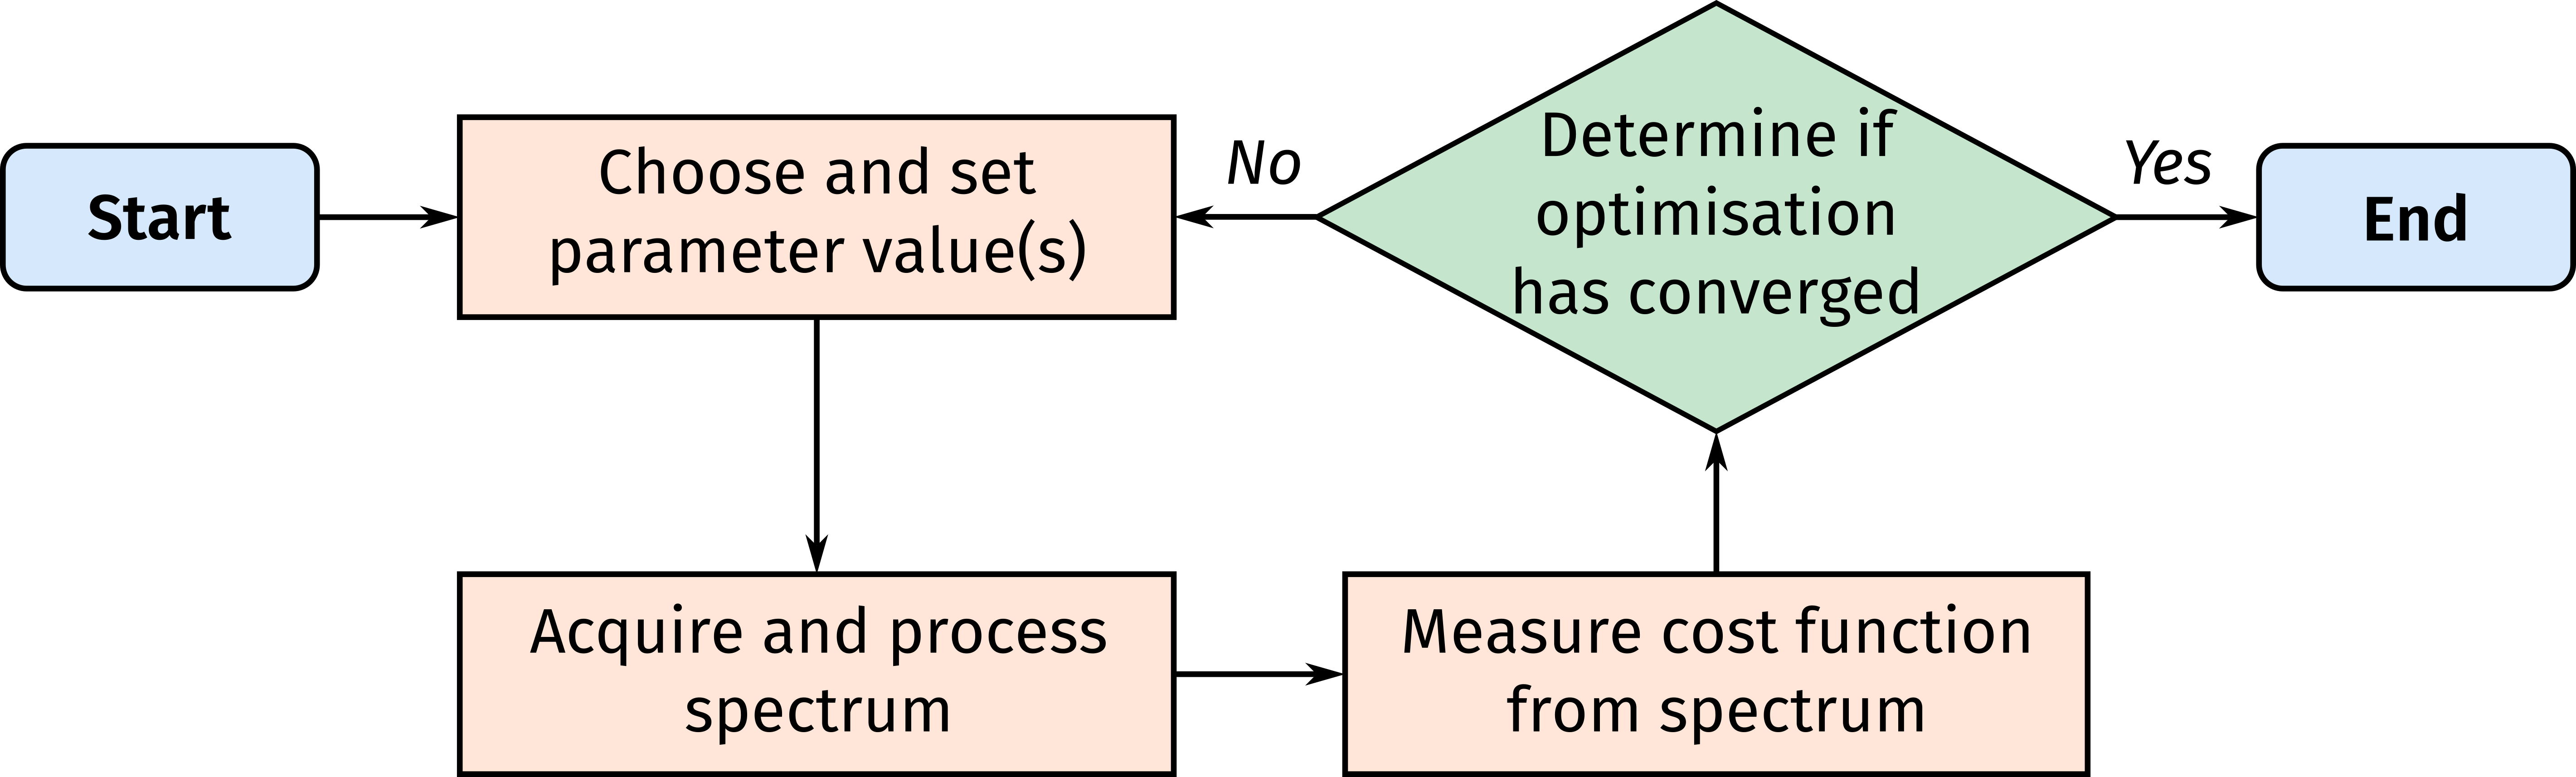
\includegraphics[]{poise/flowchart.png}
    \caption[Flowchart for POISE optimisations]{Flowchart depicting the main steps in a POISE optimisation.}
    \label{fig:poise_flowchart}
\end{figure}

Almost all aspects of this can be customised by the user, which I will now describe.
I make a distinction here between an optimisation \textit{routine}, as well as the \textit{settings} used to run these routines.
Routines consist of a series of predefined variables, such as the parameter(s) to be optimised: however, these may be optimised in different \textit{ways}, which is where the settings come in.
When discussing individual applications in \cref{sec:poise__applications}, I will make repeated reference to these components of an optimisation.

\subsection{Routines}
\label{subsec:poise__routines}

An \textit{optimisation routine}, as defined in POISE, consists of the following components:

\begin{enumerate}
    \item \textit{Name}

        This is an identifier used to refer to the entire routine, which is arbitrary, but should ideally be descriptive.

    \item \textit{Parameters}

        The parameters to be optimised.
        These are given as strings and directly correspond to TopSpin parameter names, for example, \texttt{P1} for a pulse width.

    \item \textit{Initial guess} (one per parameter)

        The point at which the optimisation is started.
        Naturally, this should represent the user's best guess at where the optimum lies.
        It is generally sensible to choose the unoptimised, `default' values for these.
        
    \item \textit{Lower} and \textit{upper bounds} (one each per parameter)

        Most parameters have a `chemically sensible' range, or alternatively, instrumental limits may sometimes restrict the range of parameter values which can be explored.

    \item \textit{Tolerances} (one per parameter)

        This loosely corresponds to the level of accuracy required for the optimisation.
        There is no point in setting this to be too small (i.e.\ requesting an overly accurate optimum), as the value of the cost function at two points too close together will likely differ only by noise.
        Furthermore, parameter values cannot be implemented with arbitrary precision on a spectrometer: the available resolution on this sets a lower bound for the tolerance (see \cref{subsec:poise__epsi} for a more concrete discussion of this).
        On the other hand, setting the tolerance to be too large may simply yield an imprecise and meaningless result.
        These conditions make it sound as if there is little room for error, but in practice getting the order of magnitude correct is usually enough (and the desired accuracy is also often reasonably clear from the context);

    \item \textit{AU programme}

        The AU programme defined here is used to acquire and process the spectrum.
        The user may leave this empty, in which case POISE automatically detects the dimensionality of the experiment and performs standard processing steps (Fourier transformation, window multiplication, phase correction, and baseline correction).
        However, this allows for almost infinite customisation of the actual spectral measurement: for example, the AU programme may call other scripts in TopSpin which create shaped pulses.

    \item \textit{Cost function}

        As before, this measures the `badness' of the spectrum thus recorded, and as before, the optimisation seeks to minimise this value.
        The cost function is written in Python 3: this design decision is considered later in \cref{subsec:poise__implementation}.
        Several cost functions which cover `typical' optimisation scenarios, such as maximising or minimising some signal intensity, come pre-installed with POISE, meaning that users do not necessarily need to write their own cost function if they are not familiar with Python.
\end{enumerate}

POISE allows users to create new routines interactively through a series of dialog boxes.
Alternatively, routines themselves can be created on-the-fly using the \texttt{poise --create} command: this is useful when some components are not known beforehand, such as if the optimum from a different optimisation is to be used as the initial point in a new one.
However, this is limited to single-parameter routines.

After being created, routines are stored in the human-readable JSON format: they can therefore be modified using any text editor.
Examples of these JSON files are presented in subsequent sections.

\subsection{Optimisation settings}
\label{subsec:poise__settings}

Once the user has defined a routine, it can then be run from the TopSpin command line using the command \texttt{poise ROUTINE\_NAME}.
However, the routine itself merely controls what parameters are being optimised: it does not specify what experiment is to be run (i.e.\ the pulse programme), nor any of the other parameters in the experiment.
These must be set by the user, and can most conveniently be stored in a TopSpin parameter set which can simply be loaded before starting the optimisation.
This flexibility means that the same \textit{type} of optimisation may be applied to different pulse sequences without having to create individual routines for each: for example, an experiment to optimise the NOE mixing time (as described in \cref{subsec:poise__noe}) can be run with different versions of the NOESY sequence depending on what is most appropriate.
Likewise, parameters such as the number of scans can be adjusted in order to run optimisations on samples with different concentrations.

Once the experiment parameters have been set up, there are a few more options which control how the optimisation is carried out:

\begin{itemize}
    \item the \texttt{-\phantom{}-maxfev} option allows the user to control the maximum number of FEs, or in other words, the maximum number of experiments run.
        If the optimisation has not converged after acquiring this many spectra, the best result so far is simply returned.
        This effectively allows the time spent on optimisation to be capped.

    \item the \texttt{-\phantom{}-quiet} option silences all output from the optimiser (the best parameters found are stored in the dataset itself after the optimisation ends, and can therefore be retrieved).
        This is useful when a POISE optimisation is to be run under automation.
        
    \item the \texttt{-\phantom{}-separate} option allows each FE to be run in a new experiment number, so that the optimisation trajectory can be analysed after its conclusion.

    \item perhaps most importantly, the \texttt{-\phantom{}-algorithm} option allows the user to choose one of three optimisation algorithms.
        I now describe these algorithms in greater detail.
\end{itemize}

\subsection{Optimisation algorithms}
\label{subsec:poise__algorithms}

As was briefly mentioned in \cref{subsec:pureshift__optim_techniques}, derivative-based optimisation algorithms cannot be used for experimental optimisations.
To be more precise, when analytical gradients are not available, derivative-based algorithms calculate gradients using a finite difference approximation:
\begin{equation}
    \label{eq:finite_difference_grad}
    \nabla f(x) \approx \frac{f(x + \varepsilon) - f(x - \varepsilon)}{2\varepsilon},
\end{equation}
where $\varepsilon$ is the step size used for the finite difference calculation.
In Nocedal and Wright\autocite{Nocedal2006}, it is shown that the error in this finite difference gradient (as compared to the true gradient) has an upper bound of
\begin{equation}
    \label{eq:finite_difference_error}
    \frac{\eta(x;\varepsilon)}{\varepsilon} + O(\varepsilon^2),
\end{equation}
where $\eta(x;\varepsilon)$ is the noise in the region $[x - \varepsilon, x + \varepsilon]$.
If $\varepsilon$ is small, the first term (the error due to noise) is large, and if $\varepsilon$ is large, the second term (which is the error due to the finite difference approximation) is large.
This means that finite difference gradients, and any algorithms which use them, are entirely unreliable in the presence of (sufficient) noise.
Instead, POISE provides a choice of three derivative-free optimisation algorithms: the \acf{nm} method\autocite{Nelder1965TCJ}, the \acf{mds} method\autocite{Torczon1989,DennisJr1991SIAMJO}, and the Py-BOBYQA trust-region method\autocite{Powell2009Proc,Cartis2019ACMTMS}.


\subsubsection{Nelder--Mead}

The NM method is a highly popular derivative-free optimisation algorithm, which maintains a set of points $\{y_1, y_2, \cdots, y_{n+1}\}$ during the optimisation, where $n$ is the number of parameters being optimised.
The convex hull of these points, $Y$, is the smallest possible set of points containing all the $y_k$ such that
\begin{equation}
    \label{eq:convex_hull}
    \forall x_1, x_2 \in Y, \forall \alpha \in [0, 1], \alpha x_1 + (1 - \alpha) x_2 \in Y,
\end{equation}
and is called a \textit{simplex}.
To provide an analogy for $n = 2$, the convex hull is the shape obtained by stretching a rubber band around three pins placed at $y_1, y_2, y_3$.
If this convex hull is nonempty---or equivalently, if the $n$ vectors $y_k - y_1$ ($2 \leq k \leq n + 1$) are linearly independent---then the simplex is called \textit{nonsingular}.
(In the $n = 2$ case, the convex hull would be empty if the three points were collinear.)

\begin{figure}[htb]
    \centering
    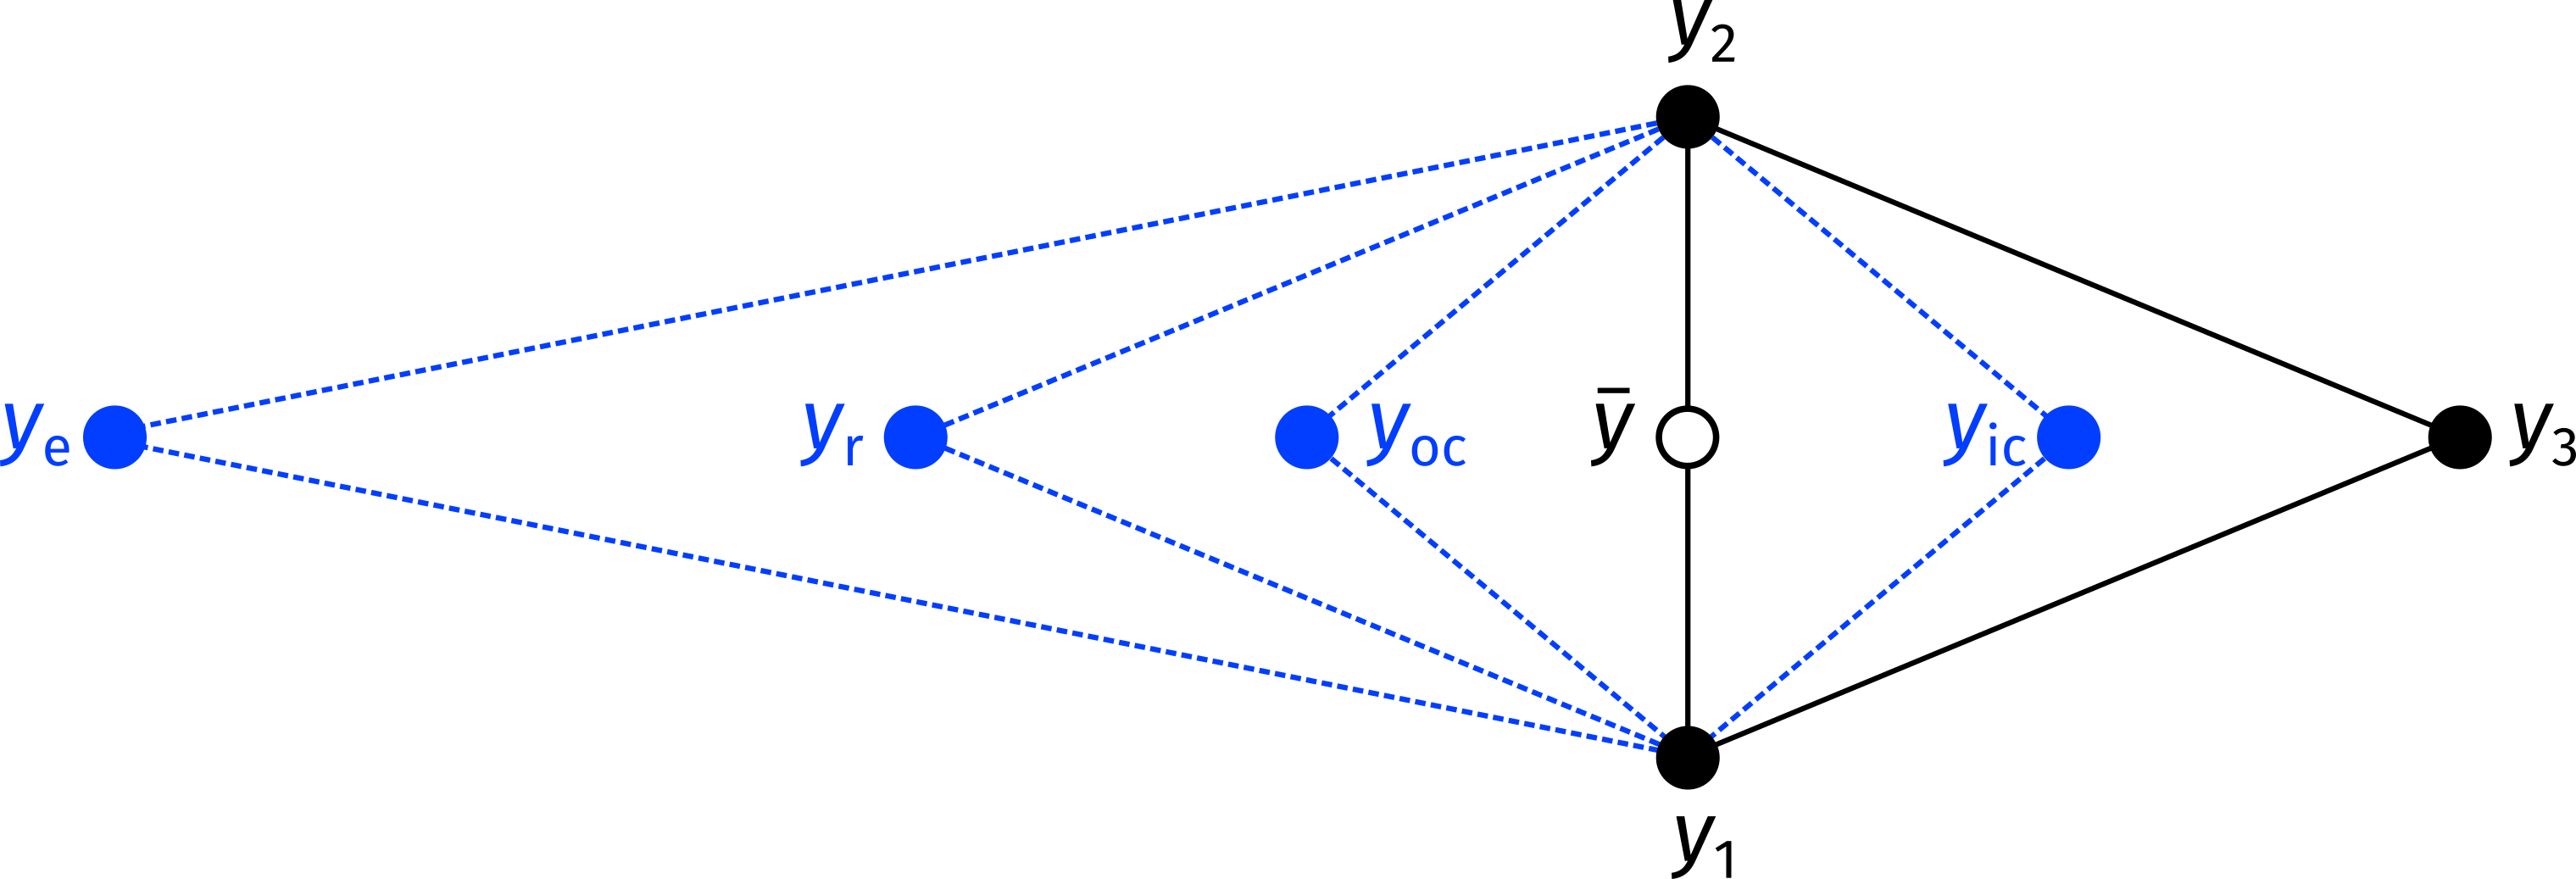
\includegraphics[]{poise/neldermead.png}
    \caption[Trial points in an iteration of the Nelder--Mead algorithm]{
        Diagram showing various points evaluated in one iteration of the Nelder--Mead algorithm (for an optimisation of two parameters).
        The solid black lines indicate the current simplex, which is assumed to be ordered such that $y_1$ is the best point (has the lowest cost function value) and $y_3$ the worst.
        The blue dots indicate the trial points which the algorithm attempts to replace $y_3$ with, and are further discussed in the text.
        Blue dashed lines indicate the simplex which would result if the corresponding trial point is accepted.
    }
    \label{fig:neldermead}
\end{figure}

The NM algorithm is in fact quite intuitive to understand.
The initial simplex is first constructed using the supplied initial point: POISE specifically uses the method of Spendley et al.\autocite{Spendley1962T}
The optimisation itself begins by measuring the cost function $f$ at every point of the simplex, and sorting the points in ascending order of cost function values (i.e.\ from best to worst), such that $f(y_1) \leq f(y_2) \leq \cdots \leq f(y_{n+1})$.
The centroid of the simplex is defined by the best $n$ points,
\begin{equation}
    \label{eq:simplex_centroid}
    \bar{y} = \sum_{i=1}^n y_i.
\end{equation}
On each iteration of the NM algorithm, we attempt to replace the worst point $y_{n+1}$  with a better point (\cref{fig:neldermead}).
The search for the new point is performed in several steps: first, the worst point is \textit{reflected} about the centroid of the simplex to obtain a new point:
\begin{equation}
    \label{eq:nm_reflect}
    y_\text{r} = \bar{y} - (y_{n+1} - \bar{y}).
\end{equation}
The value of the cost function is evaluated at this point, and is critical in determining how the algorithm proceeds.
If this reflected point falls in the middle of the pack, such that $f(y_1) \leq f(y_\text{r}) < f(y_n)$, this represents a `modest' improvement in the cost function: we simply replace the worst point with this and continue to the next iteration.

On the other hand, if the reflected point is better than all the other points (i.e.\ $f(y_\text{r}) < f(y_1)$), then we ambitiously attempt to \textit{expand} the simplex even further in that direction:
\begin{equation}
    \label{eq:nm_expand}
    y_\text{e} = \bar{y} - 2(y_{n+1} - \bar{y}).
\end{equation}
Of course, there is no guarantee that this is necessarily better than $y_\text{r}$; therefore, we choose whichever point of $y_\text{r}$ or $y_\text{e}$ had a lower value of $f$, and replace the worst point with this and continue to the next iteration.

If the reflected point is an improvement on the worst point but is no better than the remaining points, in that $f(y_n) \leq f(y_\text{r}) < f(y_{n+1})$, then the algorithm performs an \textit{outside contraction}, which resembles a half-hearted reflection:
\begin{equation}
    \label{eq:nm_outside_contract}
    y_\text{oc} = \bar{y} - (1/2)(y_{n+1} - \bar{y}).
\end{equation}
Conversely, if the reflected point is even worse than the worst point ($f(y_{n+1}) \leq f(y_\text{r})$), then this suggests that that search direction is very poor: we thus perform an \textit{inside contraction}, which uses a point halfway between the worst point and the centroid:
\begin{equation}
    \label{eq:nm_inside_contract}
    y_\text{oc} = \bar{y} + (1/2)(y_{n+1} - \bar{y}).
\end{equation}
If either of these contracted points are any better than $y_\text{r}$, then we replace the worst point in the simplex and continue to the next iteration; otherwise, we conclude that no search direction was good, and simply shrink the simplex towards the current best point by replacing each point $y_k$ with $(y_k + y_1)/2$.
In practice, these `last-resort' shrink steps occur very rarely.

Finally, convergence is signalled when for each dimension of the optimisation, the width of the simplex is smaller than the chosen optimisation tolerance.%
\footnote{The implementation of the NM algorithm in the \texttt{scipy} library only accepts a single value for the `tolerance', which is then used in all dimensions.
This is designed to be used by scaling the parameters beforehand such that the tolerance in each dimension is equal (and in fact, POISE was later updated to do so).
However, during initial development I chose instead to re-implement the NM algorithm with a convergence check which allowed for different tolerances to be specified in each dimension.}
For a multiple-parameter optimisation, this can potentially mean that extra accuracy is obtained in one of the parameters (because the simplex may have shrunk along that dimension more quickly).
However, it does guarantee that \textit{at least} the specified level of accuracy in every dimension is achieved.


\subsubsection{Multidirectional search}

In the preceding discussion, we noted that the simplex $Y$ was nonsingular if the $n$ vectors $y_k - y_1$ were linearly independent.
Equivalently, the matrix $M$ formed by concatenating these vectors
\begin{equation}
    \label{eq:simplex_matrix}
    M = \begin{pmatrix}
        y_2 - y_1, y_3 - y_1, \cdots, y_{n+1} - y_1 \\
    \end{pmatrix}
\end{equation}
must be nonsingular, i.e.\ have a nonzero determinant.
We can quantify how `close' the simplex $Y$ is to being singular, using the $l^2$ condition number of the matrix $M$, which in this context is usually referred to as the \textit{simplex condition}:
\begin{equation}
    \label{eq:simplex_condition}
    \kappa(Y) = \lVert M \rVert \lVert M^{-1} \rVert,
\end{equation}
where $\lVert M \rVert$ is the matrix norm induced by the Euclidean norm,
\begin{equation}
    \label{eq:matrix_norm}
    \lVert M \rVert = \max_{x \neq 0} \frac{\lVert Mx \rVert}{\lVert x \rVert}.
\end{equation}
A singular simplex $Y$ of course does not have a well-defined condition, since $M^{-1}$ does not exist.
However, the larger the condition of a simplex is, the closer it is to being singular.
Very loosely speaking, a long and thin simplex has a large condition number, and would be singular if its width were to go to zero.

The simplex updates made in the process of the NM algorithm mean that the simplex condition changes throughout the course of the optimisation.
This is good for achieving decreases in the cost function, since the simplex shape \textit{adapts} to the cost function being optimised.
However, if the simplex condition gets too large, it is possible that the optimisation will stall at a nonstationary point, since the search directions of the simplex are severely limited.
The MDS algorithm was proposed partially for the purpose of avoiding this ill-conditioning.\footnote{The main reason was in fact to better exploit computer parallelism, but it was also noticed that the MDS method proved to be generally more robust than NM.}

The MDS method is also simplex-based, and uses similar reflection/expansion/contraction steps as NM.
However, instead of (e.g.) reflecting a single worst point $y_{n+1}$ about the other points, it reflects all of the $n$ worst points $\{y_2, y_3, \cdots, y_{n+1}\}$ about the best point $y_1$.
This means that the shape of the simplex $Y$, and thus its condition $\kappa(Y)$, is always preserved, which provides it with much better convergence properties, as was shown by Torczon et al.\autocite{Torczon1989,Torczon1991SIAMJO}.%
\footnote{Specifically, it can be concluded that at least one of the search directions was bounded away from being orthogonal to the gradient; or in simpler (and less precise) terms, at least one of the search directions is close enough to a direction in which the cost function $f$ decreases.}
The increased reliability of the MDS algorithm over the NM algorithm was demonstrated on a variety of example optimisation problems: even in the very simple case where the cost function was simply the norm of a vector,
\begin{equation}
    \label{eq:norm_cf}
    f(y) = \lVert y \rVert,
\end{equation}
it was shown that the NM algorithm stalled when the dimension of the problem, $n$, was sufficiently large.
The value of $n$ needed to precipitate this failure depended on the problem being solved, and generally ranged from 8 to 40.
On the other hand, the MDS method proved to be robust under the same conditions, eventually converging to the optimum---although in the cases where NM \textit{did} work, the MDS method generally required more FEs.

It was this improved robustness of the MDS algorithm which prompted Goodwin et al.\autocite{Goodwin2018JMR} to use it in their (experimental) optimisation of ESR pulse shapes, and for me to later include it in POISE.
In the ESR work, the number of pulse points being optimised was 11 or 21, which fell into the regime where the MDS method would likely have better convergence properties than NM.
However, optimisations of this scale are feasible in ESR only because of the rapid relaxation and thus short experiment repetition times.
In NMR, each experiment takes a substantially longer time, and even optimisations with $n > 2$ become rather time-consuming due to the number of FEs required (the largest $n$ explored in the present work is 4).
As will be shown later, we found that the NM and MDS methods were equally reliable in our optimisations, with NM generally being faster.


\subsubsection{Py-BOBYQA}

Unlike the NM and MDS algorithm, Py-BOBYQA is not simplex-based, but is a trust-region algorithm.\autocite{Powell2009Proc,Cartis2019ACMTMS}
The fundamental idea behind a (derivative-free) trust-region method is to sample the cost function at a set of points $Y$, and construct a model $m$ through interpolation, which matches the cost function at these points:
\begin{equation}
    \label{eq:trust_region_model}
    \forall y \in Y, m(y) = f(y).
\end{equation}
The model at iteration $k$ is labelled $m_k$.
Most trust region methods use a quadratic model, and Py-BOBYQA is no exception.
This can be expressed as:
\begin{equation}
    \label{eq:trust_region_quadratic_model}
    m_k(x_k + p) = c + g^Tp + p^TGp,
\end{equation}
where $G$ is a symmetric matrix and $x_k$ is the centre of the model at iteration $k$ ($x_0$ being the user-specified initial point).
For this model to be fully determined, the set $Y$ must therefore contain $(n+1)(n+2)/2$ points in total.%
\footnote{In a derivative-based trust region method, $g$ and $G$ are determined using information from the gradient and/or Hessian.}

The algorithm maintains a \textit{trust region radius} $\Delta_k$ at each iteration, which is a measure of how reliable the model is.
The initial trust region radius, $\Delta_0$, can be arbitrarily chosen: in the case of POISE, I elected to set $\Delta_0$ to be $10$ times the desired tolerance.
The model $m_k$ is then used to calculate the next step $s_k$, which is obtained by minimising $m_k$ over all points within a radius of $\Delta_k$ from the centre $x_k$ (the \textit{trust region subproblem}):
\begin{equation}
    \label{eq:trust_region_subproblem}
    s_k = \argmin_{\lVert s \rVert \leq \Delta_k} m_k(x_k + s).
\end{equation}
Since $m_k$ is noiseless, this can be done with almost any algorithm: Py-BOBYQA uses a conjugate gradient method.
The (true) cost function is then evaluated at the trial point $x_k + s_k$, and compared against the value predicted by the model.
If the ratio of `actual improvement' to `predicted improvement' is large enough, i.e.
\begin{equation}
    \label{eq:trust_region_threshold}
    r_k = \frac{f(x_k) - f(x_k + s_k)}{m_k(x_k) - m_k(x_k + s_k)} \geq \eta
\end{equation}
for some threshold value $\eta$, then the step $s_k$ is accepted and $x_{k+1}$ is set to $x_k + s_k$, replacing the worst point in $Y$.
Additionally, the trust region radius $\Delta_k$ may be increased so that the next step(s) can be more ambitious.
Conversely, if $r_k < \eta$, then there are one of two possibilities: either the model is poorly conditioned (in that the points in $Y$ are very unevenly distributed), in which case one of the points is replaced and the model recalculataed; or the model is sufficiently well-conditioned, in which case the step is rejected, and $\Delta_k$ is decreased.

Py-BOBYQA goes beyond a standard derivative-free trust-region algorithm in further limiting the rate at which the radius $\Delta_k$ can change (amongst others).
Separately from $\Delta_k$, Py-BOBYQA also maintains a lower bound on the trust region radius $\rho_k$, and on unsuccessful iterations $\Delta_k$ is not allowed to decrease further than $\rho_k$.
This prevents $\Delta_k$ from decreasing too quickly until the algorithm is certain that $Y$ is sufficiently well-conditioned.\autocite{Powell2003MP}
Another critical feature of Py-BOBYQA is the implementation of multiple restarts, which endows it with greater robustness towards noise and also allows it to escape local minima.\autocite{Cartis2019ACMTMS,Cartis2022O}
However, the multiple-restarts feature in Py-BOBYQA was disabled in POISE as this often led to overly long optimisations.%
\footnote{Most mathematics papers on optimisation have no qualms in using hundreds or even thousands of FEs, and it is this context in which Py-BOBYQA outperforms other algorithms. Unfortunately for me, POISE works in an \textit{extremely} restrictive regime where even 50 FEs would be considered very expensive.}

Crucially, Py-BOBYQA differs from the simplex-based methods in that \textit{it cares about the actual value of the cost function}.
In the NM and MDS methods, only the relative ordering of the points in the simplex matters; it makes no difference to the algorithm whether the worst point has a cost function value of 10 or 1000.
However, in Py-BOBYQA, the value of $f$ is used in constructing the model, and thus directly influences the optimisation trajectory.
Although this is beneficial in cases where the underlying cost function is relatively well-behaved (this \textit{probably} means cases where the cost function is well described by a quadratic model\footnote{Of course, because of Taylor's theorem, every non-noisy cost function can be locally described by a quadratic model within a sufficiently small region. However, for meaningful progress to be made with noisy cost functions, the model must be built over a large enough region such that noise becomes less relevant.}), and is reflected in faster convergence rates, it can be problematic for some cost functions.
Py-BOBYQA is set as the default optimiser in POISE, but the user is strongly recommended to try the NM method as a first step when troubleshooting failed optimisations.

\section{Implementation}
\label{sec:poise/implementation}

Blah.

Flowchart.

Python 3. Blah.


\section{What POISE is not}
\label{sec:poise__notpoise}

Before moving on to cover applications of POISE, I want to make a note about several limitations of the approach chosen. 

Firstly, \textit{POISE is not specialised}.
While generality is a strength in that POISE can be applied to a diverse range of NMR experiments, it can also be a weakness.
POISE \textit{always} follows the framework in \cref{fig:poise_flowchart}: in particular, it simply seeks to find the optimum $\symbf{x}^*$, defined by
\begin{equation}
    \label{eq:poise_argmin}
    \underset{\symbf{x}}{\argmin}\, f(\symbf{x}).
\end{equation}
This rigidity in the underlying logic means that it is very conceivable that in specific instances, specialised optimisation routines which use customised strategies for data acquisition and analysis \textit{can} outperform POISE in terms of speed and/or accuracy.

A related point is that on each function evaluation, the only bits of information retained are the parameters $\symbf{x}$ and the value of the cost function $f(\symbf{x})$.
The spectral data itself is not stored anywhere:\footnote{In principle, it \textit{could} be. There is nothing stopping me from implementing something to store previous spectra; it was just not the original motivation behind POISE.} thus, it is not possible to perform (for example) an `optimisation' which collects scans until a certain SNR is reached, or one which collects $t_1$ increments of a 2D spectrum and performs non-uniform sampling (NUS) processing until the signal to artefact ratio is sufficiently high.
In particular, I want to distinguish POISE from other types of `optimisations' reported in the literature, which typically \textit{accumulate} data points until a given confidence level is reached (e.g.\ through a model-fitting procedure).
Such procedures have been performed before in the contexts of (for example) relaxation measurements\autocite{Song2018JMR,Tang2019SR} and undersampling in multidimensional NMR\autocite{Eghbalnia2005JACS,Hansen2016ACIE,BrukerSmartDriveNMR}.

Secondly, \textit{POISE is not a processing software}.
Although POISE can in theory be used for optimisation of processing parameters (for example, by changing the `acquisition' AU programme to perform only processing tasks), this usage is not considered here.
Such optimisations can be more efficiently carried out on a personal computer, without requiring access to a spectrometer.

Finally, \textit{POISE is not a panacea}.
It should be noted that there is always an inherent tradeoff against the time required for the optimisation itself.
For example, it makes little sense to spend several minutes optimising the sensitivity of a pulse--acquire experiment: the time could simply be used to improve the SNR by collecting more scans.
There is also the critical---though undeniably subjective---question of whether the optimisation is \textit{worth it}: even if better results can be obtained in relatively short times, does this provide a substantial benefit over a `compromise' value in a default parameter set?%
\footnote{Of course, even though it is nowadays fashionable for authors to imply that their publications possess \textit{great impact}, a similar argument can be applied to \textit{many} scientific discoveries. To use an example from the next chapter, is it really necessary to acquire NOAH spectra when one can just acquire the standalone 2D experiments? I have seen arguments on both sides---some people simply do not need the speedups provided and do not want to spend the time to set up or troubleshoot new experiments.}
I do not profess to have a definitive answer to this, and I leave the reader to form their own conclusions in the specific contexts where they may consider using POISE.
In any case, for practical use, it is imperative to make sure that the optimisation is either fast, or solves a problem which cannot simply be tackled through signal averaging in the same amount of time.
It is my hope that this is (broadly) true of the examples shown.

\section{Applications}
\label{sec:poise__applications}

In this section, I cover a number of scenarios in which POISE can be used.
These are generally ordered from simple to complex, and progressively show how the features in POISE can be used to customise optimisation procedures.

All POISE optimisations run in this chapter were performed five times to check for potential reproducibility issues.
Due to noise in the cost function, these optimisations are not deterministic, and the optima obtained typically span a range.
Where possible, this range is quoted in all the results shown in this chapter.


\subsection{Pulse width calibration}
\label{subsec:poise/applications/pulsecal}

\texttt{popt} vs \texttt{pulsecal}

\subsection{Ernst angle optimisation}
\label{subsec:poise__ernst}

Often, in a simple 1D pulse--acquire spectrum it is not hugely important to know the exact \ang{90} pulse width: instead, it is more valuable to optimise the sensitivity per unit time of the spectrum.

\subsubsection{Optimisation setup}

\begin{figure}[htb]
    \centering
    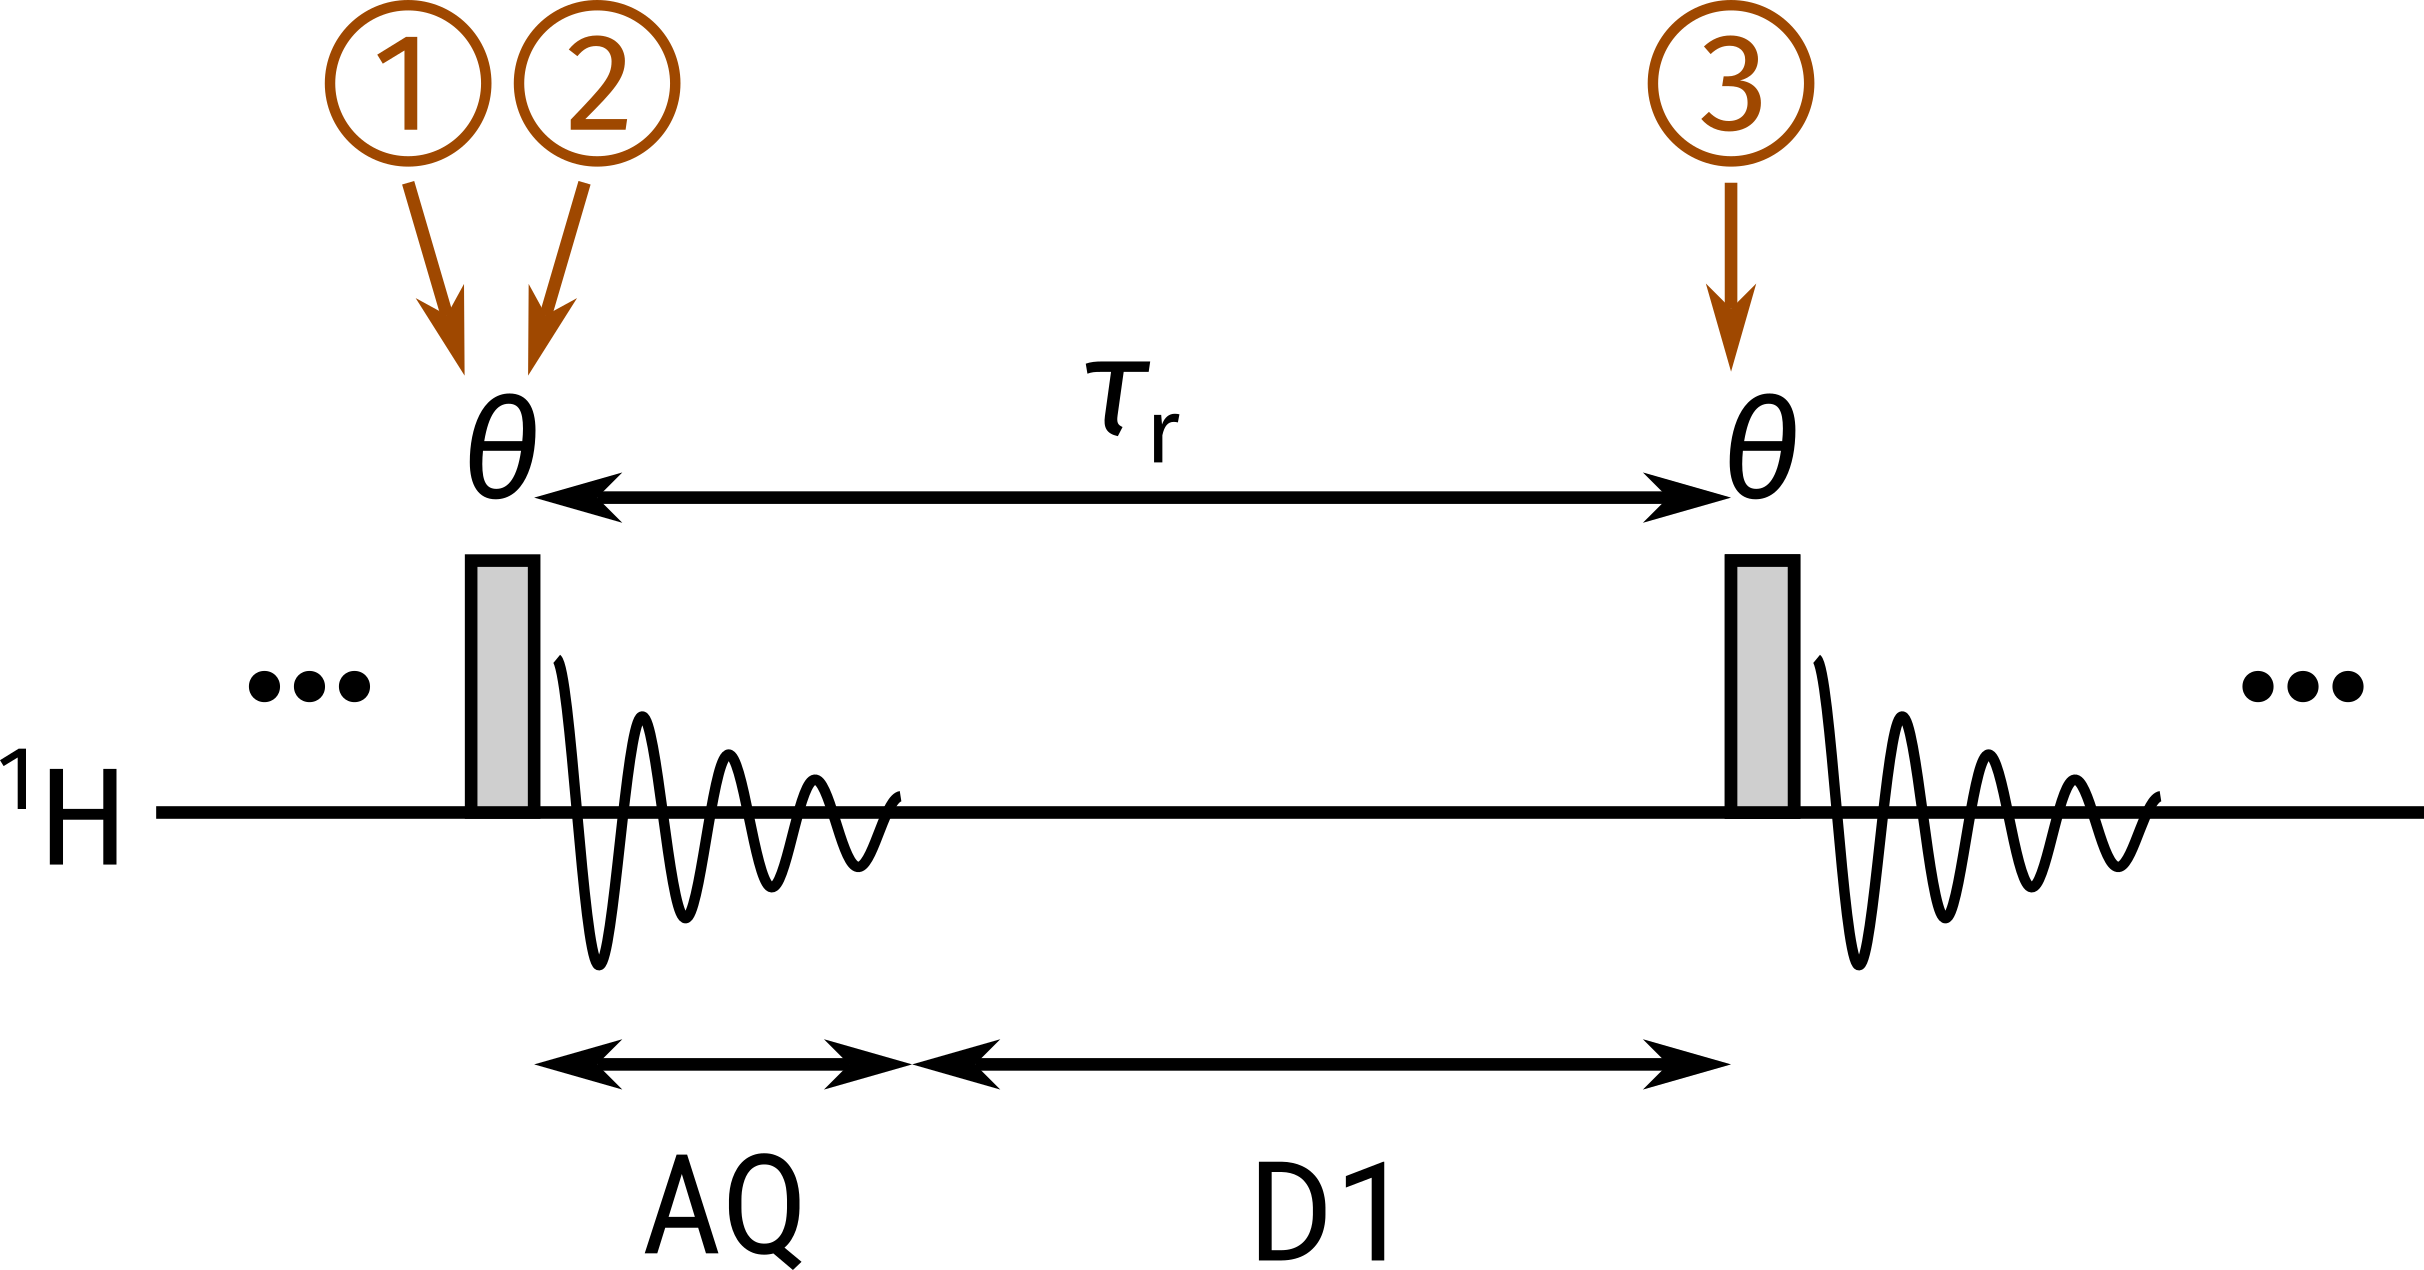
\includegraphics[]{pp/poise/zg_repeated.png}%
    \caption[Steady-state pulse--acquire experiment]{Steady-state pulse--acquire experiment. The excitation flip angle is $\theta$, and the repetition time between experiments is $\taur$.}
    \label{fig:zg_ernst}
\end{figure}

Before launching straight into how this may be obtained through optimisation, it is instructive to first consider which parameters are worth optimising.
For a pulse--acquire experiment (\cref{fig:zg_ernst}), the repetition time is the sum of the acquisition time \texttt{AQ} plus the recovery delay \texttt{D1}; the flip angle $\theta$ is controlled via the pulse width \texttt{P1}.
We assume that the experiment has been repeated enough times to reach a \textit{steady state}, that is, the amount of $z$-magnetisation prior to the excitation pulse (point \circled{1}) is a constant $M_{z,\text{ss}}$.
Application of the excitation pulse leads to a signal scaling as $M_{z,\text{ss}}\sin\theta$, and residual (unexcited) longitudinal magnetisation of $M_{z,\text{ss}}\cos\theta$ at point \circled{2}.
After the repetition time $\taur$ (point \circled{3}), it can be shown using the Bloch equations\autocite{Bloch1946PR} that the $z$-magnetisation recovers to
\begin{equation}
    \label{eq:z_magn_ernst1}
    M_{z,0}(1 - c) + cM_{z,\text{ss}}\cos\theta,
\end{equation}
where $c = \exp(-\taur/T_1)$ and $M_{z,0}$ is the initial, equilibrium $z$-magnetisation (before the experiment begins).
Since the experiment has reached a steady state, points \circled{1} and \circled{3} are equivalent: thus, we have that
\begin{equation}
    \label{eq:z_magn_ernst2}
    M_{z,0}(1 - c) + cM_{z,\text{ss}}\cos\theta = M_{z,\text{ss}},
\end{equation}
which can be rearranged to give
\begin{equation}
    \label{eq:z_magn_ernst3}
    \frac{M_{z,\text{ss}}}{M_{z,0}} = \frac{1 - c}{1 - c\cos\theta}.
\end{equation}
The signal amplitude $s$ therefore scales as
\begin{equation}
    \label{eq:z_magn_ernst4}
    s = \frac{(1 - c)}{1 - c\cos\theta} \cdot \sin\theta,
\end{equation}
and is maximised when $\md s/\md \theta = 0$, the solution of which is the celebrated \textit{Ernst angle}\autocite{Ernst1966RSI}:
\begin{equation}
    \label{eq:ernst_angle}
    \theta_\text{E} = \arccos{c} = \arccos\left[\exp\left(-\frac{\taur}{T_1}\right)\right].
\end{equation}
In general, $T_1$ and hence $\theta_\text{E}$ varies across the different spins in a given sample, so some degree of compromise is required in order to maximise sensitivity for all peaks.

Naively, we may then consider fixing $\taur$ and optimising \texttt{P1} to locate the Ernst angle (or to be precise, the pulse width which corresponds to the Ernst angle, since that is the only quantity we really care about).
This is generally true.
However, we can go one step further, because $\taur$ itself is comprised of two parameters, and the sensitivity \textit{per unit time} may be affected by varying $\taur$.
Since the signal scales as $1/\taur$ (a shorter $\taur$ means more repetitions per unit time) but the noise scales only as $\sqrt{1/\taur}$, the sensitivity per unit time is
\begin{equation}
    \label{eq:z_magn_ernst5}
    S = \frac{(1 - c)\sin\theta}{(1 - c\cos\theta)\sqrt{\taur}}.
\end{equation}
Assuming that $\theta$ is always set to the respective Ernst angle for different $\taur$, it can be shown that the best sensitivity per unit time is attained when $\taur \to 0$.\autocite{Waugh1970JMS,Traficante1992CMR}
Of course, this limit is not physically possible: $\taur$ comprises the acquisition time which must be nonzero.
However, it does imply that \texttt{AQ} should be kept as short as possible, and \texttt{D1} set to zero, as shown in \cref{fig:ernst_sensitivity}.

\begin{figure}[htb]
    \centering
    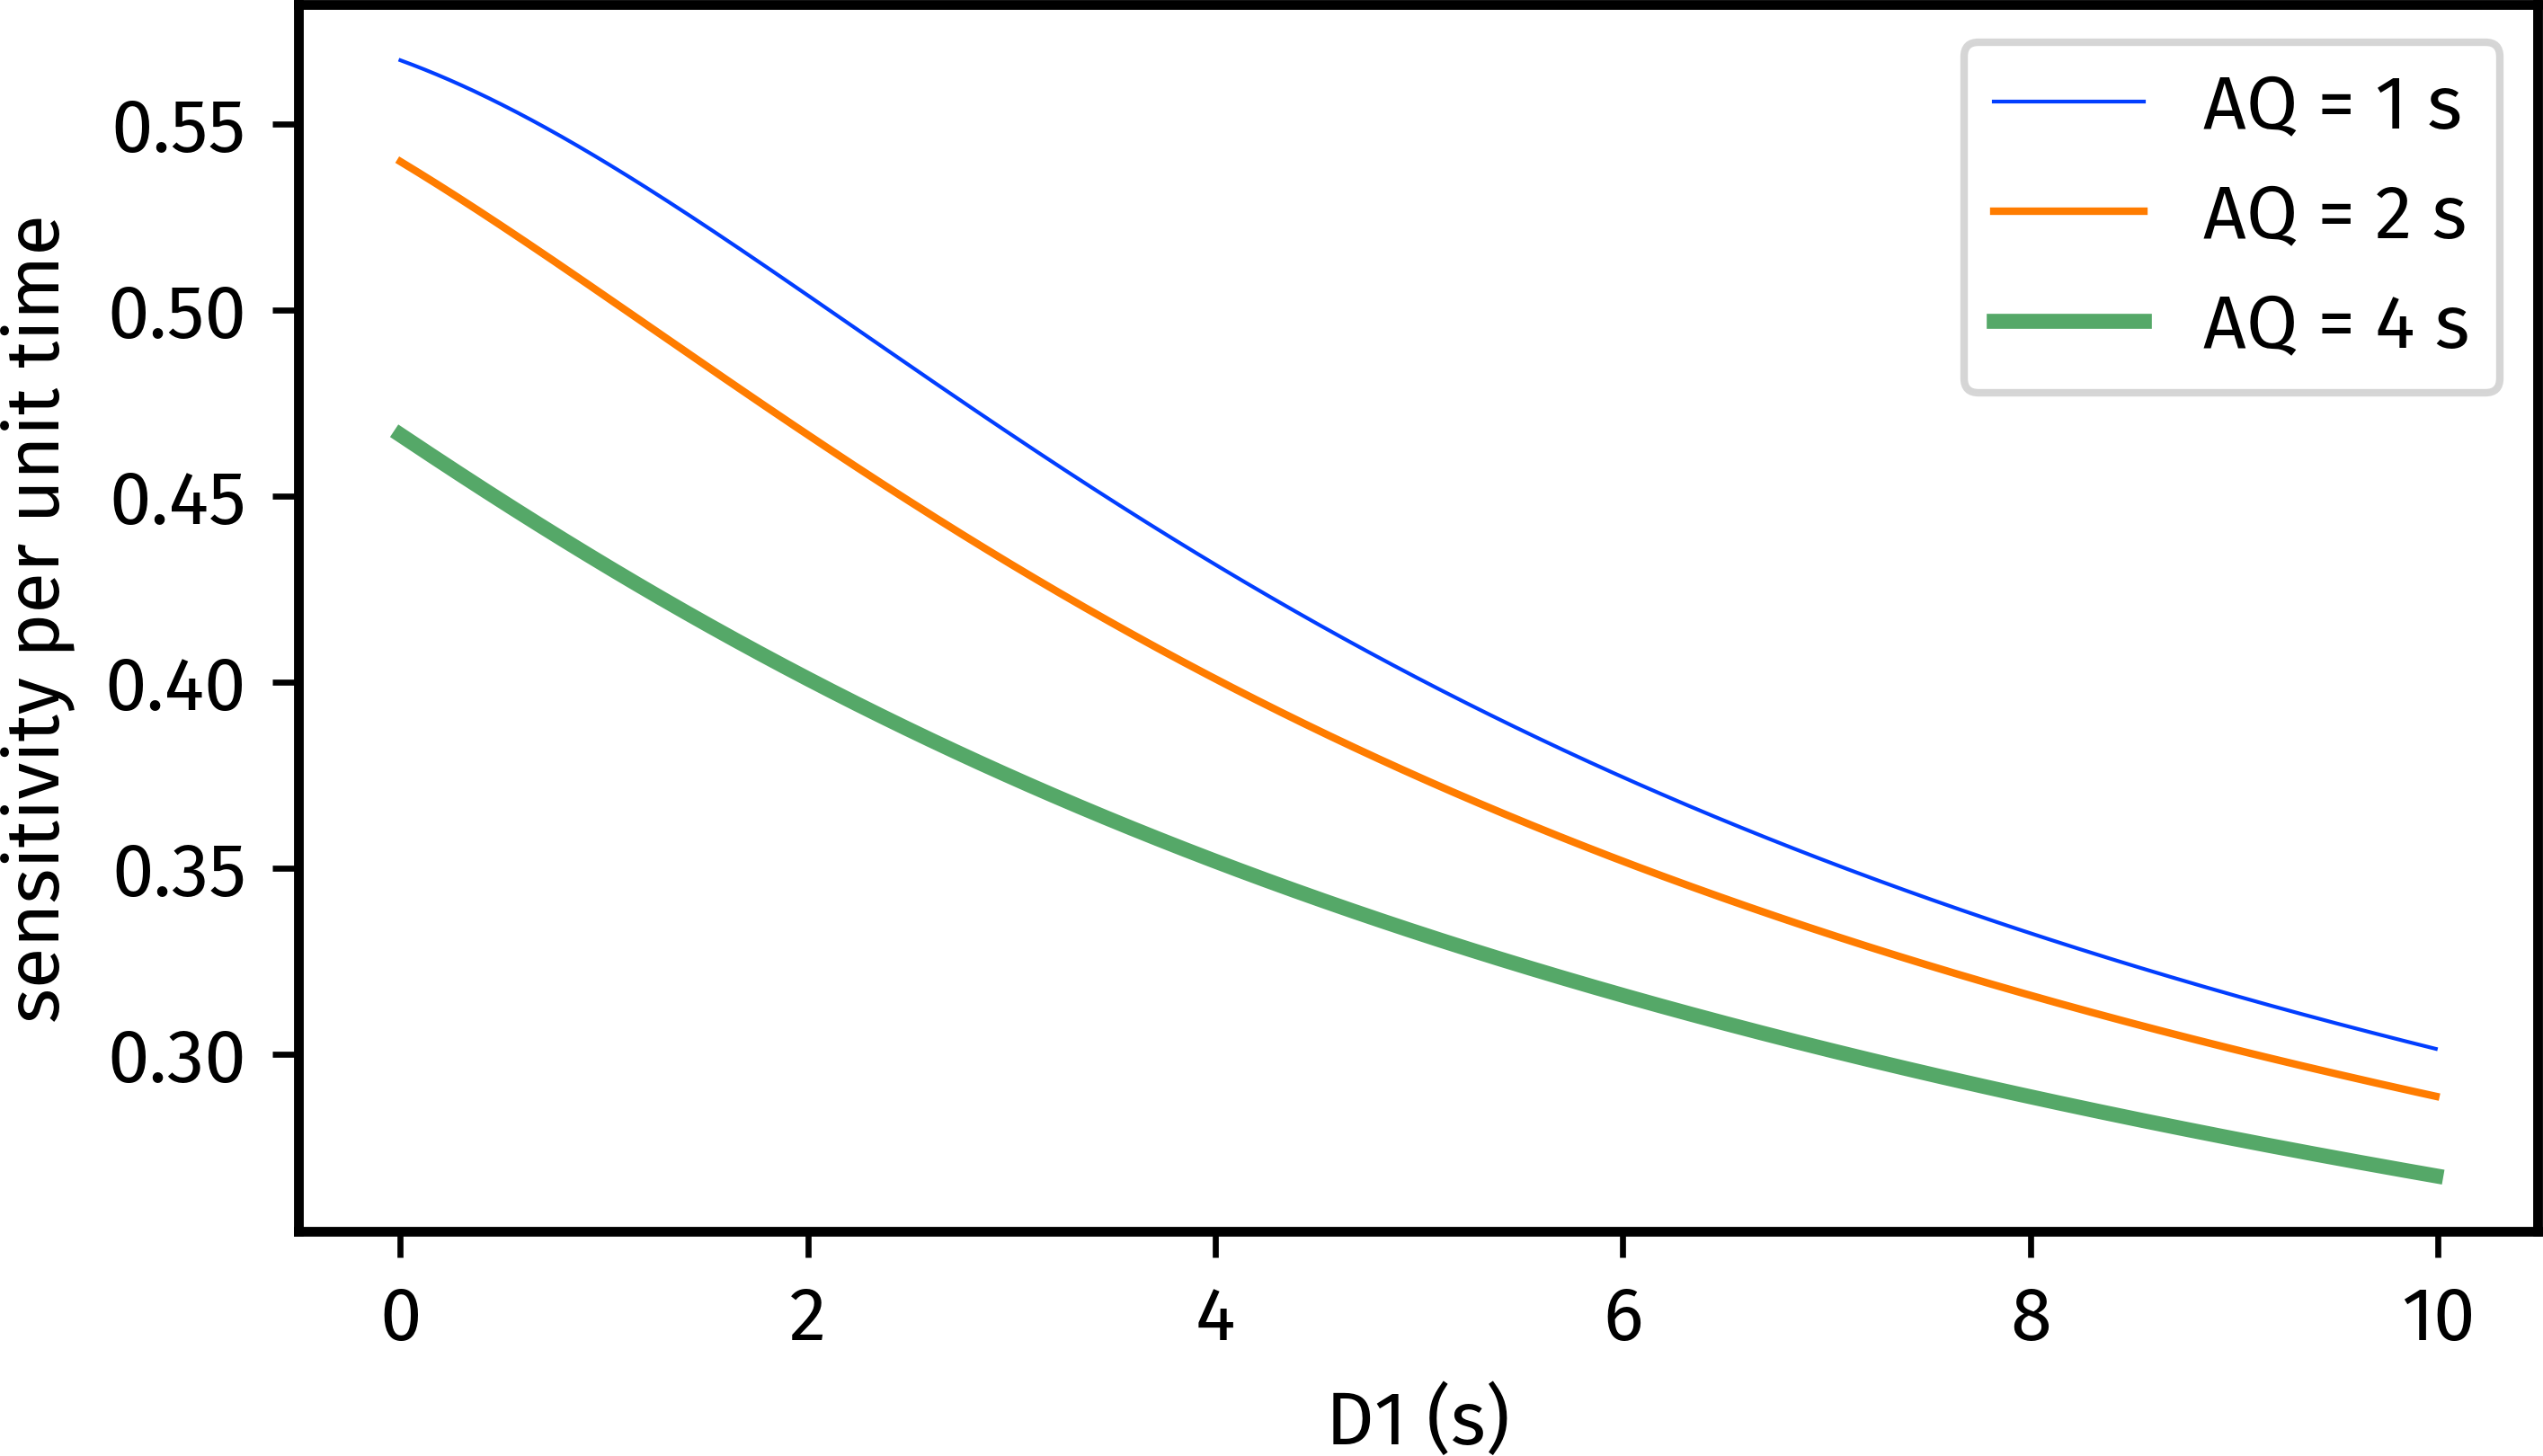
\includegraphics[]{poise/ernst_sensitivity.png}%
    \caption[Sensitivity per unit time as a function of \texttt{AQ} and \texttt{D1}]{Sensitivity per unit time as a function of \texttt{AQ} and \texttt{D1}, assuming that an Ernst angle excitation pulse is used. $T_1$ was set to \SI{1.5}{\s}.}
    \label{fig:ernst_sensitivity}
\end{figure}

Knowing this, we can then set up a meaningful optimisation routine.
We seek to optimise the pulse width \texttt{P1} such that the intensity of the real part of the spectrum is maximised (corresponding to a \texttt{maxrealint} cost function).
In practice, I took the extra step of calibrating the \ang{90} pulse width (as per the previous section) and modifying the pulse programme such that the flip angle could be specified as the parameter \texttt{CNST20}: this is not generally necessary and is only useful for evaluating the results, as will be shown later.
As per the above analysis, I set \texttt{AQ} and \texttt{D1} to be \SI{1.2}{\s} and 0 respectively.
The number of scans (\texttt{NS}) can be set to 1, but unlike in the pulse width calibration (\cref{subsec:poise__pulsecal}), we must use enough dummy scans to ensure that a steady-state signal intensity is recorded: in practice I set \texttt{DS=4}.
This means that each FE, and thus the overall optimisation, requires a slightly longer time than the pulse width calibrations previously shown.


\subsubsection{Optimisation results}

The Ernst angle optimisation was run with two different spectral regions of interest: firstly, on all the aromatic and olefinic peaks in the sample of ferulic acid (\cref{tbl:poise_ernst_fivepeaks}), and secondly, on only the peak at \SI{6.79}{\ppm} (\cref{tbl:poise_ernst_onepeak}).
(This spectral region can be selected using the TopSpin \texttt{dpl} command, which stores the bounds using the parameters \texttt{F1P} and \texttt{F2P}: all built-in cost functions respect these two parameters.)
Generally, optimisations could be completed in under two minutes.
The optima found for these two optimisations are different: this is because the former searches for a compromise Ernst angle which balances $T_1$ of all peaks within the region, and the latter optimises only for one $T_1$.

\begin{table}[htb]
    \hbadness=10000
    \centering
    \begin{tabular}{ccccc}
        \toprule
        Entry & Algorithm & Optimum found ($^\circ$) & FEs   & Time taken (\si{\s}) \\
        \midrule
        1     & NM        & 67.5--73.1               & 9--13 & 91--132              \\
        2     & MDS       & 67.5--73.1               & 9     & 90--92               \\
        3     & BOBYQA    & 70.1--70.7               & 7     & 70--71               \\
        \bottomrule
    \end{tabular}
    \caption[Ernst angle optimisations on a range of peaks]{
        Ernst angle optimisation, performed on all aromatic and olefinic peaks in ferulic acid (between 6 and \SI{8}{\ppm}).
        The POISE routine used here is: \mintinline[breaklines]{json}{{"name": "ernst", "pars": ["cnst20"], "lb": [10.0], "ub": [90.0], "init": [30.0], "tol": [3.0], "cf": "maxrealint", "au": "poise_1d"}}.
        \datacode{5F-210619}
    }
    \label{tbl:poise_ernst_fivepeaks}
\end{table}

\begin{table}[htb]
    \hbadness=10000
    \centering
    \begin{tabular}{ccccc}
        \toprule
        Entry & Algorithm & Optimum found ($^\circ$) & FEs   & Time taken (\si{\s}) \\
        \midrule
        1     & NM        & 60.0--67.5               & 9--11 & 91--111              \\
        2     & MDS       & 65.6--67.5               & 11    & 110--111             \\
        3     & BOBYQA    & 60.0--65.2               & 6--7  & 59--71               \\
        \bottomrule
    \end{tabular}
    \caption[Ernst angle optimisations on only one peak]{
        Ernst angle optimisations on the peak at \SI{6.79}{\ppm} in ferulic acid.
        The POISE routine is the same as in \cref{tbl:poise_ernst_fivepeaks}, but the spectral region under optimisation was set to be 6.71--\SI{6.87}{\ppm}
        The theoretical optimum, as given in \cref{tbl:ernst_invrec}, is \ang{61.6}.
        \datacode{5F-210619}
    }
    \label{tbl:poise_ernst_onepeak}
\end{table}

To determine the accuracy of the optima found, rather than performing a reference grid search as in \cref{subsec:poise__pulsecal}, I measured $T_1$ of each of these peaks using a typical gradient-enhanced inversion--recovery experiment, and calculated the theoretical Ernst angles from this (\cref{tbl:ernst_invrec}).
The first optimisation, which should yield essentially a weighted average of the five Ernst angles, appears at first glance to be biased towards larger values.
However, this can be rationalised by the fact that that a flip angle larger than $\theta_\text{E}$ is less detrimental to sensitivity compared to one that is smaller (this can be seen by plotting \cref{eq:z_magn_ernst4}).
On the other hand, the second optimisation yields an accurate value for the relevant peak (number 4 in \cref{tbl:ernst_invrec}), at least to within the specified tolerance of \ang{3}.

\begin{table}[htb]
    \centering
    \begin{tabular}{ccccc}
        \toprule
        Peak & \proton{} chemical shift (ppm) & $T_1$ (\si{\s}) & $\theta_\text{E}$ ($^\circ$) & $T_1\ln 2$ (\si{\s})\\
        \midrule
        1 & 7.49 & 1.750 & 59.8 & 1.213 \\
        2 & 7.27 & 0.977 & 73.0 & 0.677 \\
        3 & 7.08 & 1.279 & 67.0 & 0.887 \\
        4 & 6.79 & 1.615 & 61.6 & 1.119 \\
        5 & 6.36 & 1.415 & 64.6 & 0.981 \\
        \bottomrule
    \end{tabular}
    \caption[$T_1$ values for ferulic acid]{
        $T_1$ and corresponding Ernst angles for each peak in ferulic acid, calculated for a repetition time of \SI{1.20}{\s}.
        The values of $T_1 \ln 2$ are also provided here, in anticipation of the inversion--recovery experiments performed in \cref{subsec:poise__invrec}.
        \datacode{5F-210619}
    }
    \label{tbl:ernst_invrec}
\end{table}

Finally, it is worth considering whether this optimisation is truly worth it.
\proton{} pulse--acquire spectra already have a very high intrinsic sensitivity, and in the two minutes taken to optimise the flip angle, one could easily just acquire (around) 64 more scans, at which point knowledge of the Ernst angle would cease to be useful.
It \textit{may} be more useful for nuclei which have lower sensitivity, such as \carbon{}: I did not evaluate this possibility.
However, it must be borne in mind that a low-sensitivity experiment will also require more scans per FE, which leads to a corresponding increase in the optimisation time.

In my estimation, a more useful application of this optimisation routine would be to use it to determine an average $T_1$ value for a group of peaks.
This could then be used to inform the choice of recovery delay for multidimensional experiments\autocite{Reynolds2002JNP,Burns2021MRC} or quantitative NMR experiments\autocite{Pauli2005JNP,Giraudeau2014MRC}.
It is, however, possible to more directly obtain $T_1$ values from an inversion--recovery experiment, which I describe next.

\subsection{Inversion--recovery}
\label{subsec:poise__invrec}


\subsubsection{Optimisation setup}

\begin{figure}[htb]
    \centering
    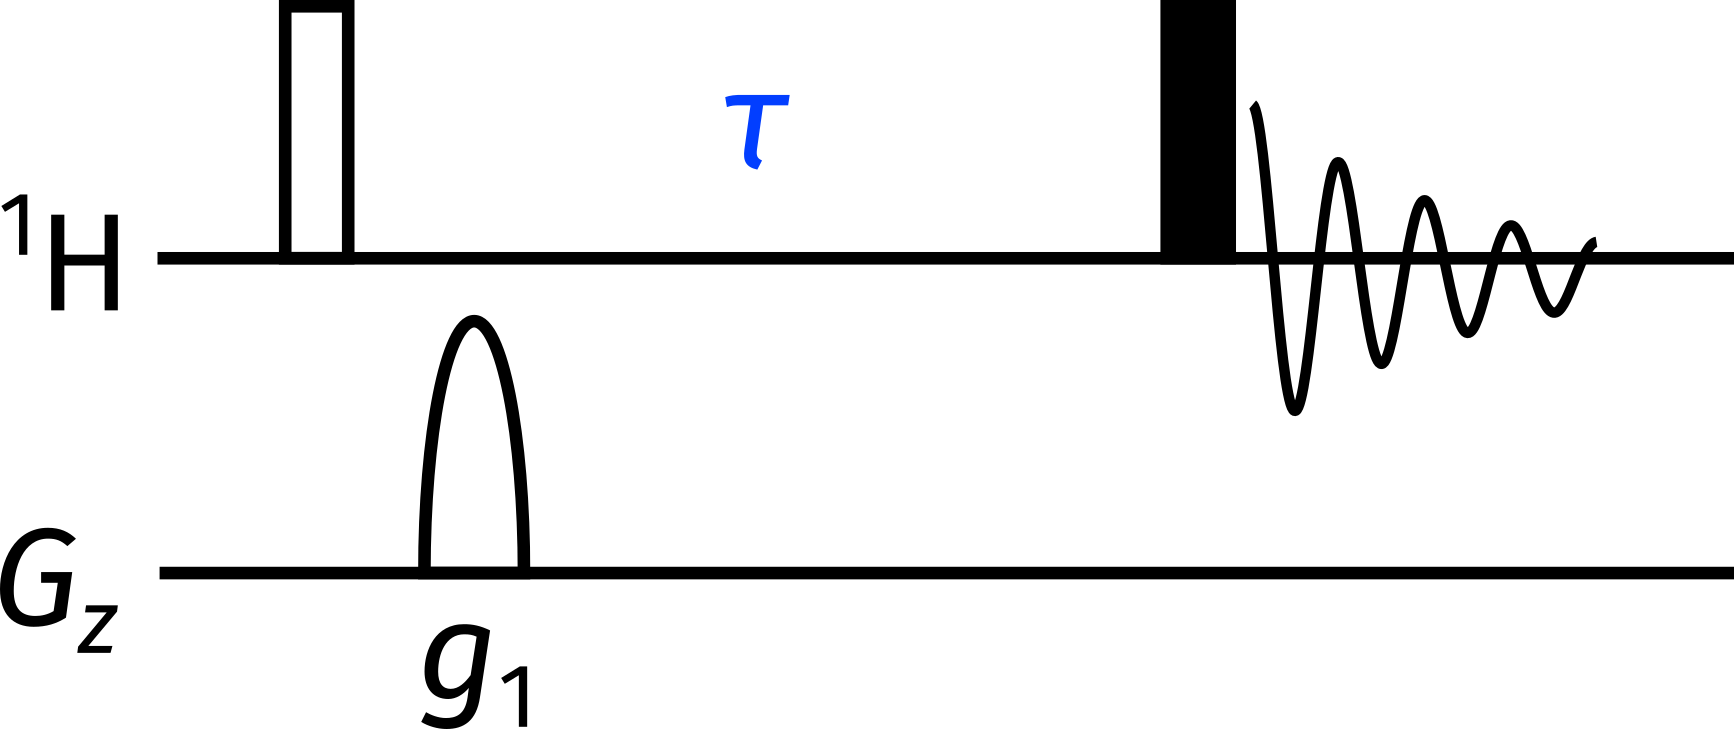
\includegraphics[]{pp/poise/invrec.png}%
    \caption[Inversion--recovery pulse sequence]{Inversion--recovery pulse sequence.}
    \label{fig:poise_invrec}
\end{figure}

If what we really want to measure is $T_1$ for a particular peak (or a set of peaks), a more direct way is to perform an inversion--recovery experiment (\cref{fig:poise_invrec}).
This can either be recorded in a 2D form where the $\tau$ delay is incremented and the resulting intensities fit to an exponential curve, or in an iterative fashion by searching for the null in spectral intensity, which occurs at $\tau = T_1\ln 2$: this latter option is particularly suited to optimisation.
The delay $\tau$ was specified as the parameter \texttt{D27}, and the \texttt{zerorealint} cost function used here is just the absolute value of the integral over the region of interest: an ideal null would have a cost function value of 0.
\Cref{tbl:ernst_invrec} provides the theoretical values of $T_1 \ln 2$, which were calculated using the more accurate 2D fitting procedure.

A slight drawback of using this method, compared to the Ernst angle optimisations in the previous section, is that the recovery delay must be sufficiently long to allow for complete relaxation between FEs: in this case, I used a \texttt{D1} of \SI{5}{\s}.
On the other hand, this also means that dummy scans are no longer needed: I therefore set \texttt{DS=0} and \texttt{NS=1}.


\subsubsection{Optimisation results}

Just as in the Ernst angle optimisations, these were performed twice, once on the entire 6--\SI{8}{\ppm} region and once on just a single peak (note that this time, the chosen peak is at \SI{7.08}{\ppm}), or peak 3 in \cref{tbl:ernst_invrec}).
The results are shown in \cref{tbl:invrec_fivepeaks,tbl:invrec_onepeak}.
The former correctly yields an `averaged' value over the five peaks, and the latter closely matches the theoretical value for the peak in question.

\begin{table}[htb]
    \hbadness=10000
    \centering
    \begin{tabular}{ccccc}
        \toprule
        Entry & Algorithm & Optimum found (\si{\s}) & FEs    & Time taken (\si{\s}) \\
        \midrule
        1     & NM        & 0.938--0.969            & 14--16 & 204--235             \\
        2     & MDS       & 0.956--0.975            & 16     & 233--235             \\
        3     & BOBYQA    & 0.953--0.971            & 9--11  & 130--160             \\
        \bottomrule
    \end{tabular}
    \caption[Inversion--recovery optimisations on a range of peaks]{
        Inversion--recovery optimisations on all aromatic and olefinic peaks in ferulic acid (between 6 and \SI{8}{\ppm}.
        The POISE routine used here is: \mintinline[breaklines]{json}{{"name": "invrec", "pars": ["d27"], "lb": [0.35], "ub": [1.75], "init": [0.6], "tol": [0.01], "cf": "zerorealint", "au": "poise_1d"}}.
        \datacode{5F-210619}
    }
    \label{tbl:invrec_fivepeaks}
\end{table}

\begin{table}[htb]
    \hbadness=10000
    \centering
    \begin{tabular}{ccccc}
        \toprule
        Entry & Algorithm & Optimum found (\si{\s}) & FEs   & Time taken (\si{\s}) \\
        \midrule
        1     & NM        & 0.863--0.875            & 14    & 202--205             \\
        2     & MDS       & 0.863--0.869            & 14    & 203--204             \\
        3     & BOBYQA    & 0.862--0.873            & 9--10 & 128--145             \\
        \bottomrule
    \end{tabular}
    \caption[Inversion--recovery optimisations on only one peak]{
        Inversion--recovery optimisations on the peak at \SI{7.08}{\ppm} in ferulic acid.
        The POISE routine is the same as in \cref{tbl:poise_ernst_fivepeaks}, but the spectral region under optimisation was set to be 7.02--\SI{7.15}{\ppm}.
        The theoretical optimum (from \cref{tbl:ernst_invrec}) is \SI{0.887}{\s}.
        \datacode{5F-210619}
    }
    \label{tbl:invrec_onepeak}
\end{table}

The only downside of these optimisations would then be the time required, which is on the order of 2--4 minutes.
Although this is less time than required for a full 2D inversion--recovery experiment, POISE has the drawback that an optimisation can only be run on one peak at a time.
Thus, if the aim is to determine $T_1$ for all peaks, then the 2D experiment may well end up being faster.
On top of that, there are many other ways to measure $T_1$ which are faster than a full 2D inversion--recovery experiment and almost certainly also faster than POISE.\autocite{Christensen1974JPC,Homer1985JMR,Loening2003JMR,Smith2013CPC,Wei2021JOC}
However, no explicit comparisons were performed in this work.

\subsection{NOE mixing time}

Stuff

\subsection{ASAP-HSQC excitation delay}
\label{subsec:poise__asaphsqc}

The next example of a POISE optimisation is the ASAP-HSQC experiment\autocite{SchulzeSunninghausen2014JACS,SchulzeSunninghausen2017JMR}: here, I use it to again illustrate the new possibilities which custom cost functions enable.
In the ASAP-HSQC experiment (\cref{fig:asaphsqc_pulseq}), an HSQC spectrum is recorded using only \carbon{}--bound proton magnetisation, and the \carbont{}--bound (`bulk') proton magnetisation is returned to the equilibrium $+z$ axis (i.e.\ the $I_z$ state).
In this way, instead of having a conventional recovery delay, the \carbon{}--\proton{} magnetisation can be directly replenished using isotropic mixing, which causes transfer of $z$-magnetisation from bulk protons.
The elision of the recovery delay from the sequence thus leads to significantly shorter experiment durations: in one of the more extreme examples, an HSQC spectrum could be recorded within 7 seconds.
This separation of different `magnetisation pools' is conceptually very similar to that in NOAH experiments (\cref{subsec:noah__magpools}), and in anticipation of that, I use the notation \magn{C} and \magnnot{C} to represent magnetisation belonging to protons coupled and not coupled to \carbon{} respectively.

\begin{figure}[htb]
    \centering
    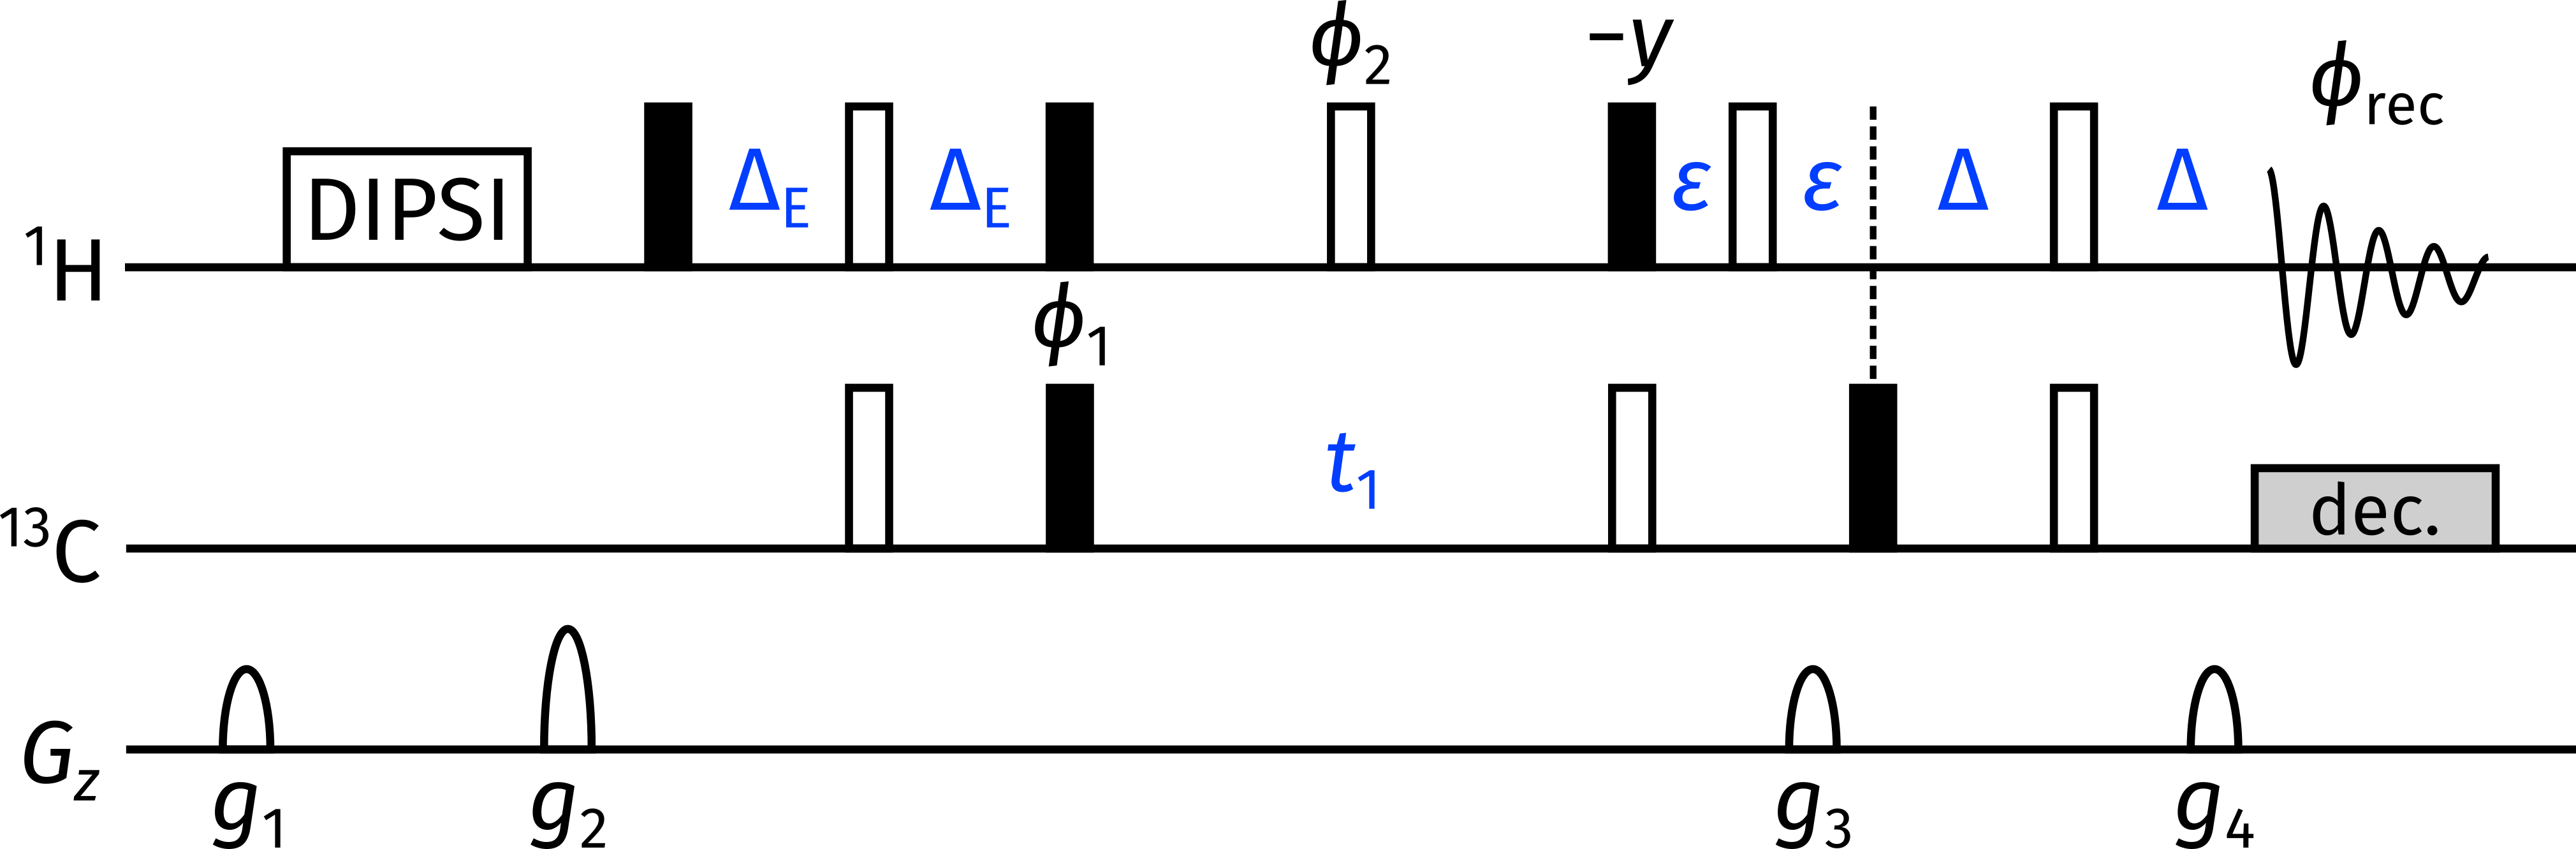
\includegraphics[]{pp/poise/asaphsqc.png}%
    \caption[ASAP-HSQC pulse sequence]{
        ASAP-HSQC pulse sequence.
        Phase cycling is performed using $\phi_1 = (x, -x)$, $\phi_2 = (x, x, -x, -x)$, and $\phi_{\symup{rec}} = (x, -x, x, -x)$.
        Gradient amplitudes are as follows: $g_1 = 33\%$, $g_2 = 43\%$, and for echo--antiecho selection, $(g_3, g_4) = (59.9\%, 80\%)$ and $(63.9\%, 80\%)$ respectively.
        The delay $\Delta$ is set to $1/(4 \cdot \oneJ{CH})$; the delay $\DeltaE$ was optimised as described in the text.
        The BIBOP, BEBOP, and BURBOP optimal control pulses\autocite{Kobzar2004JMR,Kobzar2008JMR,Kobzar2012JMR} were used for \proton{} \ang{180} pulses and all \carbon{} pulses; for more details, refer to the original paper by Luy and coworkers\autocite{SchulzeSunninghausen2014JACS}.
    }
    \label{fig:asaphsqc_pulseq}
\end{figure}

By modifying the length of the delay $\DeltaE$ in the initial INEPT block, it is possible to adjust the proportion of the \magn{C} magnetisation excited during the sequence: the remainder is stored along $z$.
The delay $\DeltaE$ can be related to an \textit{effective flip angle}, $\thetaeff$, through
\begin{equation}
    \label{eq:asaphsqc_ernst_angle}
    \thetaeff = 2\pi J \DeltaE.
\end{equation}
where $J\/$ is here short for $\oneJ{CH}$.
This partial excitation means that the signal is decreased by a factor of $\sin\thetaeff$, but means that on the next scan or increment, there is a larger pool of \magn{C} magnetisation to start from.
The combination of these factors means that there is an optimum $\DeltaE$ which yields the greatest steady-state signal.
Equivalently, we can define an `effective J-coupling', $\Jeff$, for which the INEPT delay is optimised:
\begin{equation}
    \label{eq:asaphsqc_j_eff}
    \DeltaE = \frac{1}{4 \Jeff} \quad\Longleftrightarrow\quad \Jeff = \frac{\pi J}{2\thetaeff},
\end{equation}
and we can search for the ideal $\Jeff$ to maximise the sensitivity of the ASAP-HSQC spectrum.

Notice that this is entirely analogous to the Ernst angle previously discussed in \cref{subsec:poise__ernst}.
However, here, the magnetisation is being recovered partly through isotropic mixing and partly through relaxation during the FID.
This makes an analytic description of the ASAP-HSQC experiment rather more complicated (although it has been studied before\autocite{Koos2019JMR}).
Directly optimising the excitation delay $\DeltaE$ with POISE, which circumvents the theory entirely, is therefore an attractive option for practical day-to-day use.


\subsubsection{Optimisation setup}

Given the analysis above, it is extraordinarily easy to set up the optimisation: the parameter being optimised is $\Jeff$, and the initial point chosen is a `compromise' $\oneJ{CH}$ value of \qty{150}{\Hz}.
Although generally it is not a good idea to use a 2D experiment as part of the FE, in this specific case it is acceptable because the ASAP-HSQC has such a short running time.
In this case, we simply take the projection of the 2D ASAP-HSQC onto the $F_2$ axis, integrate it, and take the negative of that to obtain the cost function.

A reference grid search was performed so that I could later verify the optimisation results (\cref{fig:asaphsqc_scan}).
The exact point where the crosspeak intensities are maximised is not obvious: generally, the signal increases up until $\Jeff \approx \qty{230}{\Hz}$, after which it plateaus off.
In a similar fashion to the NOE optimisations (\cref{subsec:poise__noe}), we may therefore consider any value above this to be `correct'.

\begin{figure}[htb]
    \centering
    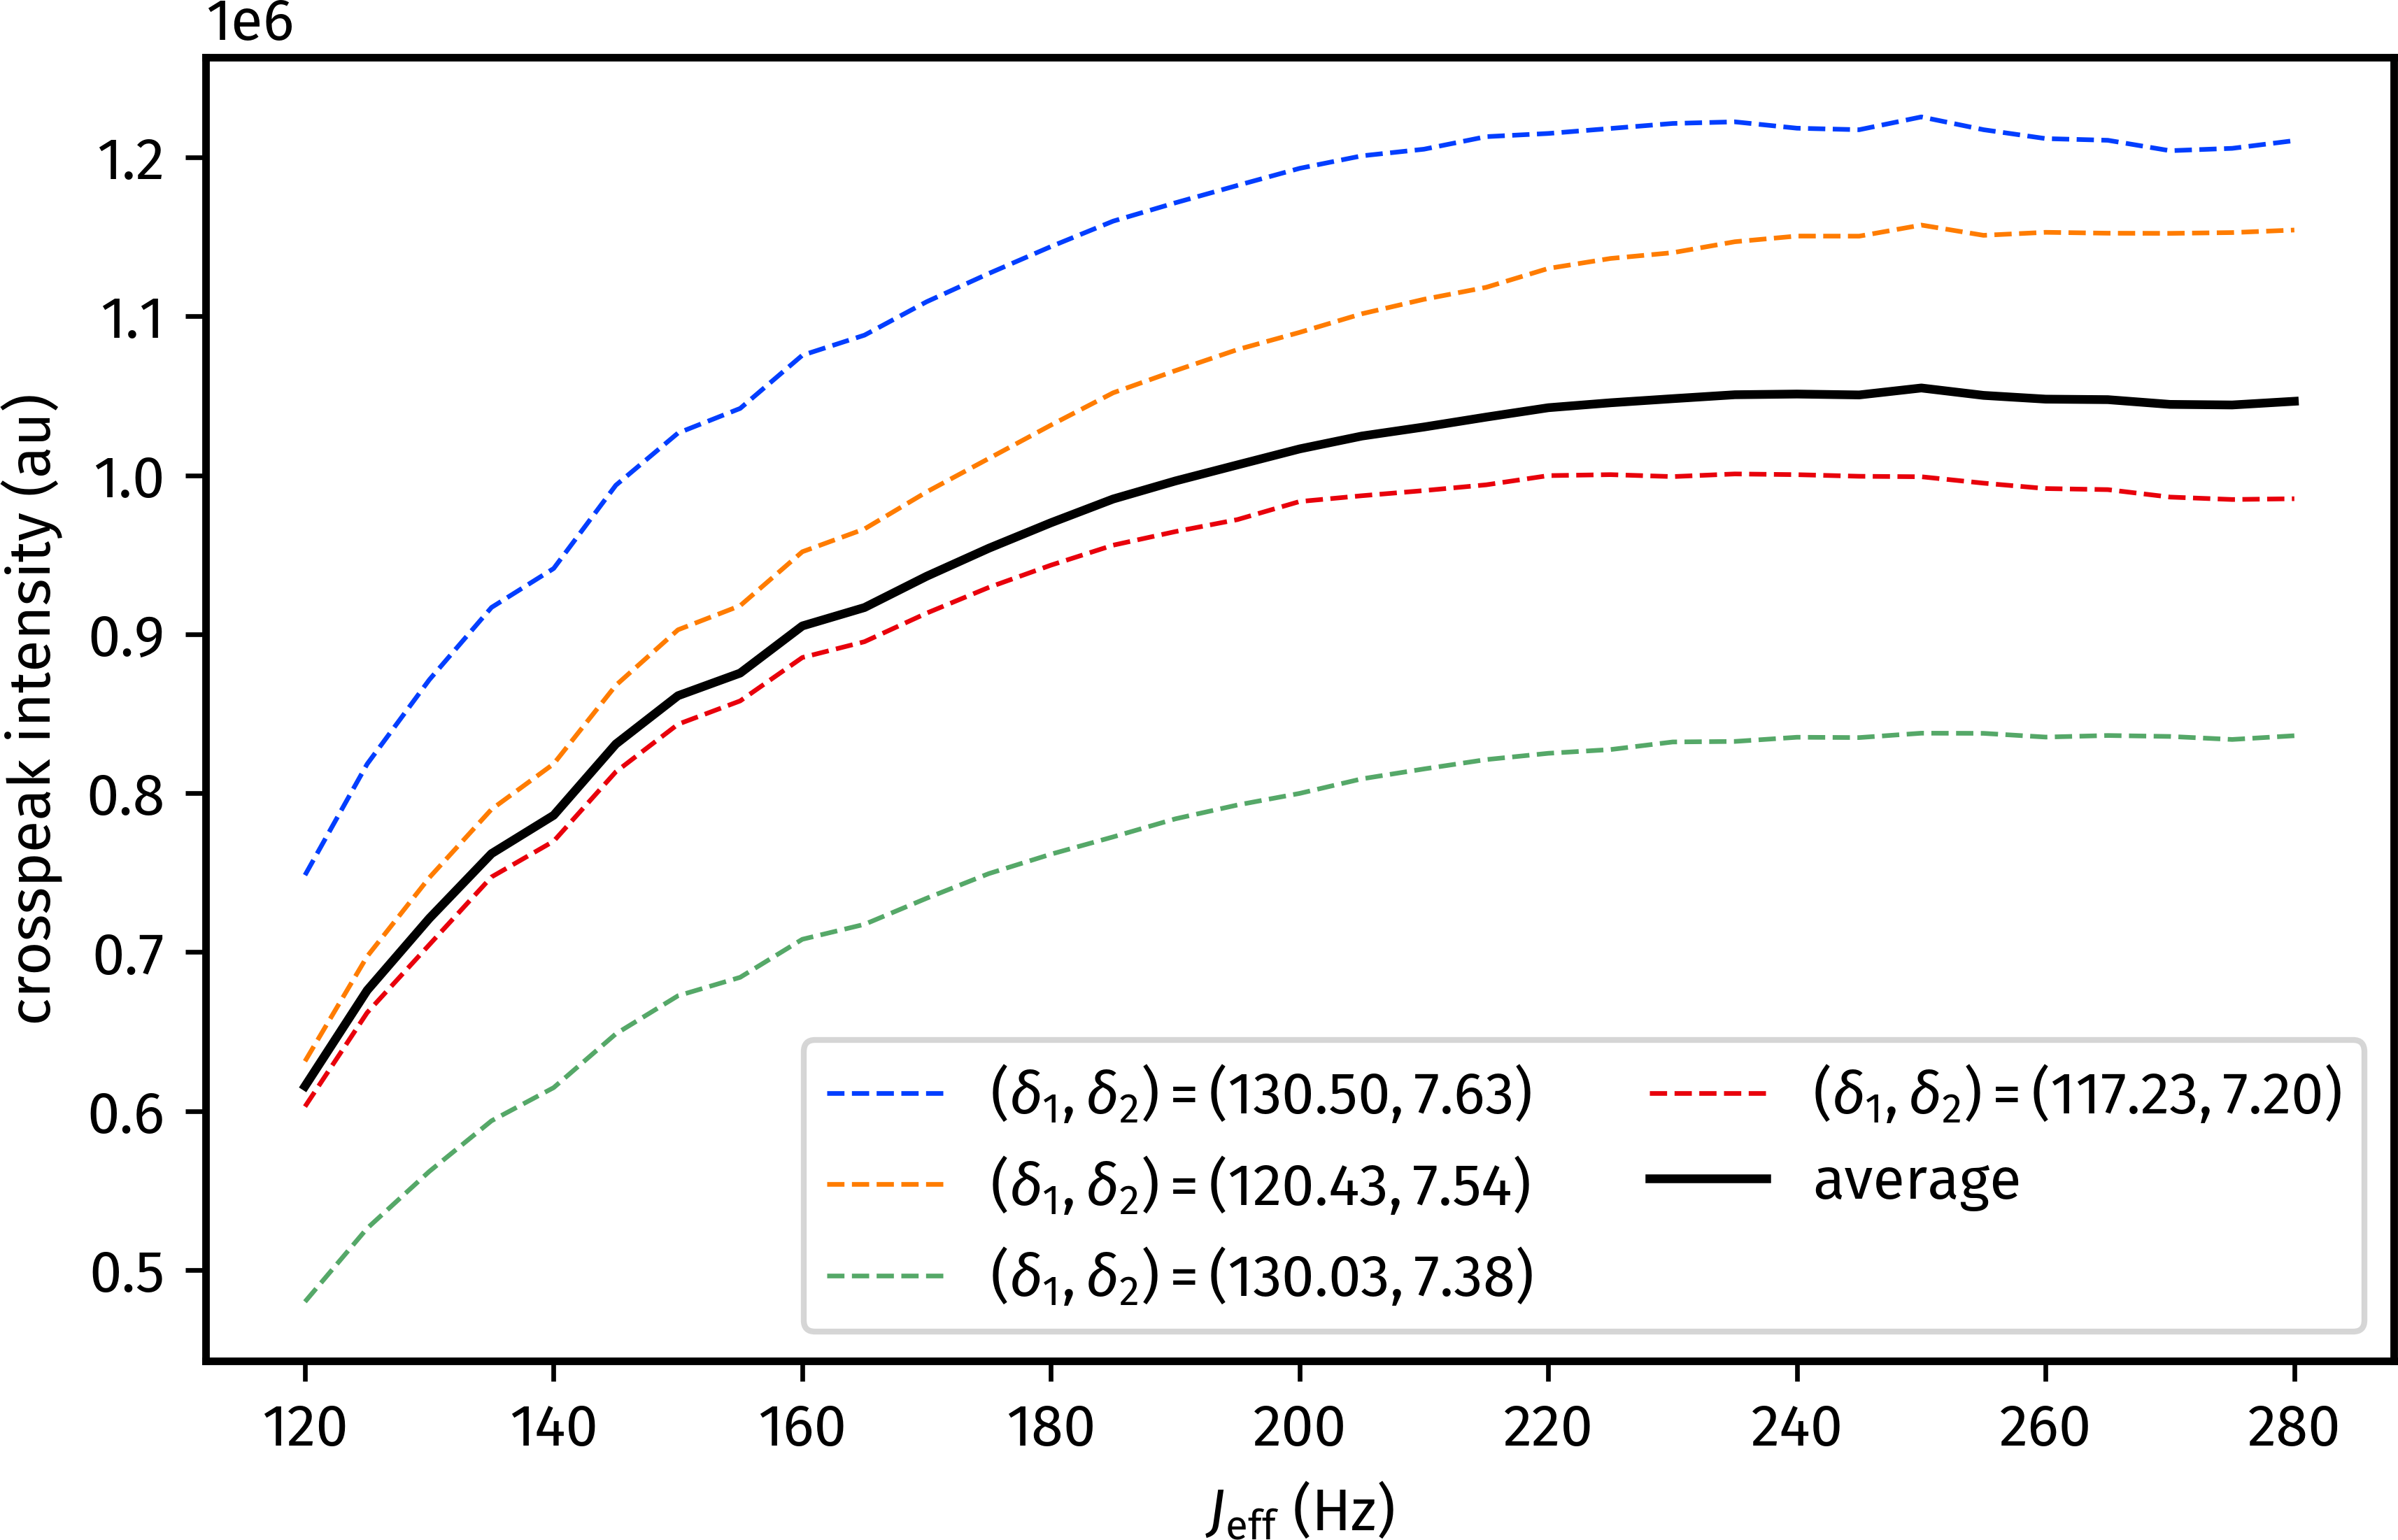
\includegraphics[]{poise/asaphsqc_scan.png}%
    \caption[Reference grid search for ASAP-HSQC excitation delay]{
        Reference grid search showing how the ASAP-HSQC signal intensity for the 3-fluorophenylboronic acid sample varies with $\Jeff$.
        \datacode{7B-200722}
    }
    \label{fig:asaphsqc_scan}
\end{figure}

To speed up the optimisation, optimisations were run using a `low-quality' ASAP-HSQC spectrum with only 32 $t_1$ increments.
A recovery delay of \qty{0.1}{\s} was used.

\subsubsection{Optimisation results}

\begin{table}[htb]
    \hbadness=10000
    \centering
    \begin{tabular}{ccccc}
        \toprule
        Entry & Algorithm & Optimum found (\unit{\Hz}) & FEs  & Time taken (\unit{\s}) \\
        \midrule
        1     & NM        & 250.0--256.3            & 8--9 & 169--195             \\
        2     & MDS       & 237.5--243.8            & 8    & 171--179             \\
        3     & BOBYQA    & 229.8--245.6            & 4--7 & 114--157             \\
        \bottomrule
    \end{tabular}
    \caption[ASAP-HSQC INEPT delay optimisations]{
        ASAP-HSQC INEPT delay optimisations.
        The POISE routine used was: \mintinline[breaklines]{json}{{"name": "asaphsqc", "pars": ["cnst3"], "lb": [120.0], "ub": [280.0], "init": [150.0], "tol": [10.0], "cf": "asaphsqc", "au": "poise_2d"}}.
        \datacode{7B-200722}
    }
    \label{tbl:poise_asaphsqc}
\end{table}

\begin{figure}[htb]
    \centering
    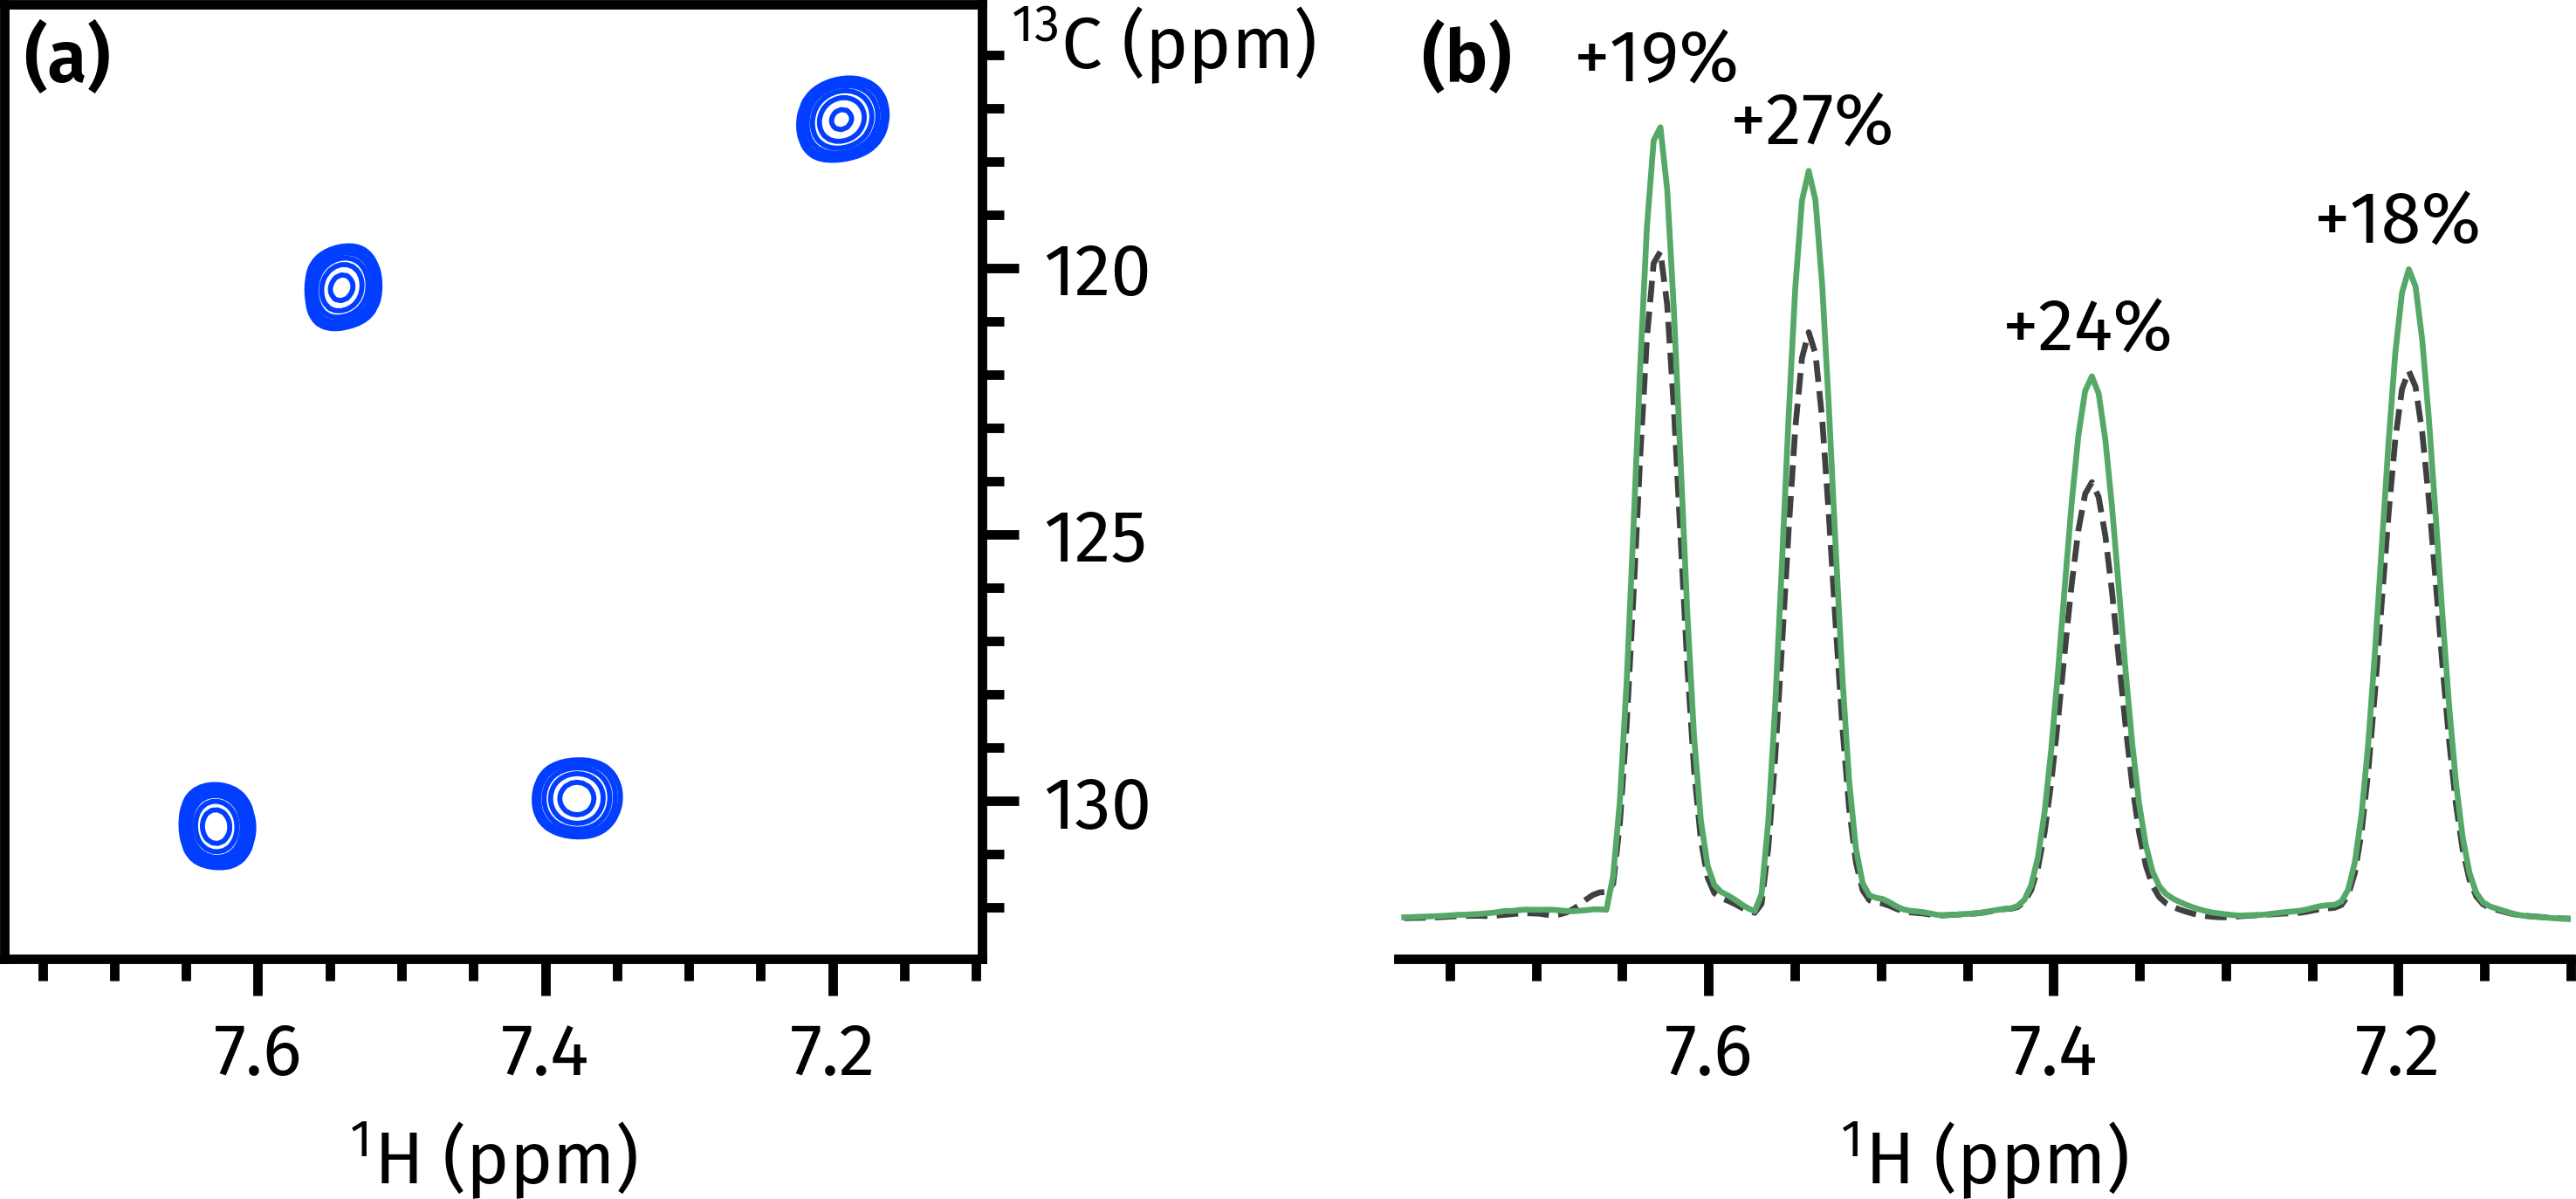
\includegraphics[]{poise/asaphsqc_spec.png}%
    {\phantomsubcaption\label{fig:asaphsqc_spec_spec}}%
    {\phantomsubcaption\label{fig:asaphsqc_spec_proj}}%
    \caption[Projections of ASAP-HSQC spectra before and after optimisation]{
        \textbf{(\subref*{fig:asaphsqc_spec_spec})} ASAP-HSQC spectrum of the 3-fluorophenylboronic acid sample.
        \textbf{(\subref*{fig:asaphsqc_spec_proj})} Projections of the ASAP-HSQC spectra before (grey dotted line, using $\Jeff = \qty{150}{\Hz}$) and after (green dotted line, using $\Jeff = \qty{245}{\Hz}$) optimisation of the INEPT delay.
        Sensitivity increases for each peak are indicated.
        \datacode{7B-200722}
    }
    \label{fig:asaphsqc_spec}
\end{figure}

The results from the POISE optimisations are collated in \cref{tbl:poise_asaphsqc}.
As can be seen, even though the FE involves acquisition of a 2D spectrum, the optimisation itself completes in just 2--3 minutes, correctly converging to $\Jeff$ values in the region of around \qty{240}{\Hz}.
When re-evaluated on a `full' ASAP-HSQC experiment with 64 $t_1$ increments (\cref{fig:asaphsqc_spec_spec}),%
\footnote{The \carbon{} resonances of interest in this compound fall within a very small window, so relatively few $t_1$ increments are needed.}
the optimisation yielded an 18--27\% improvement in the sensitivity of the ASAP-HSQC spectrum, as shown in \cref{fig:asaphsqc_spec_proj}.

In fact, this specific example is not particularly impressive in itself.
The ASAP-HSQC experiment shown in \cref{fig:asaphsqc_spec_spec} takes only around 45 seconds to acquire, so simply repeating it two or three more times would yield a similar or even larger increase in SNR.
However, this argument may easily be swung in the opposite direction if more $t_1$ increments were to be used, such as 256 for a more `typical' \carbon{} spectral window, or even more if extremely high $F_1$ resolution is desired (the original paper\autocite{SchulzeSunninghausen2014JACS} provides an example of a three-hour ASAP-HSQC experiment where 16384 $t_1$ increments were recorded to differentiate two peaks separated by \qty{3}{\Hz} in $F_1$).

\subsection{Ultrafast NMR}
\label{subsec:poise__epsi}

The final example of a single-parameter POISE optimisation is also the most complicated: it pertains to the EPSI acquisition technique, which was previously introduced in \cref{sec:pureshift__epsidosy}.
EPSI acquisition allows signals from different slices of the sample to be simultaneously detected in a single FID, and (in liquid-state NMR) has most famously been used in the context of \textit{ultrafast} 2D experiments\autocite{Frydman2002PNASUSA,Pelupessy2003JACS,Frydman2003JACS,Tal2010PNMRS,Giraudeau2014ARAC,Gouilleux2018ARNMRS}, where the $t_1$ evolution is spatially encoded and read out using the EPSI technique.

\begin{figure}[htb]
    \centering
    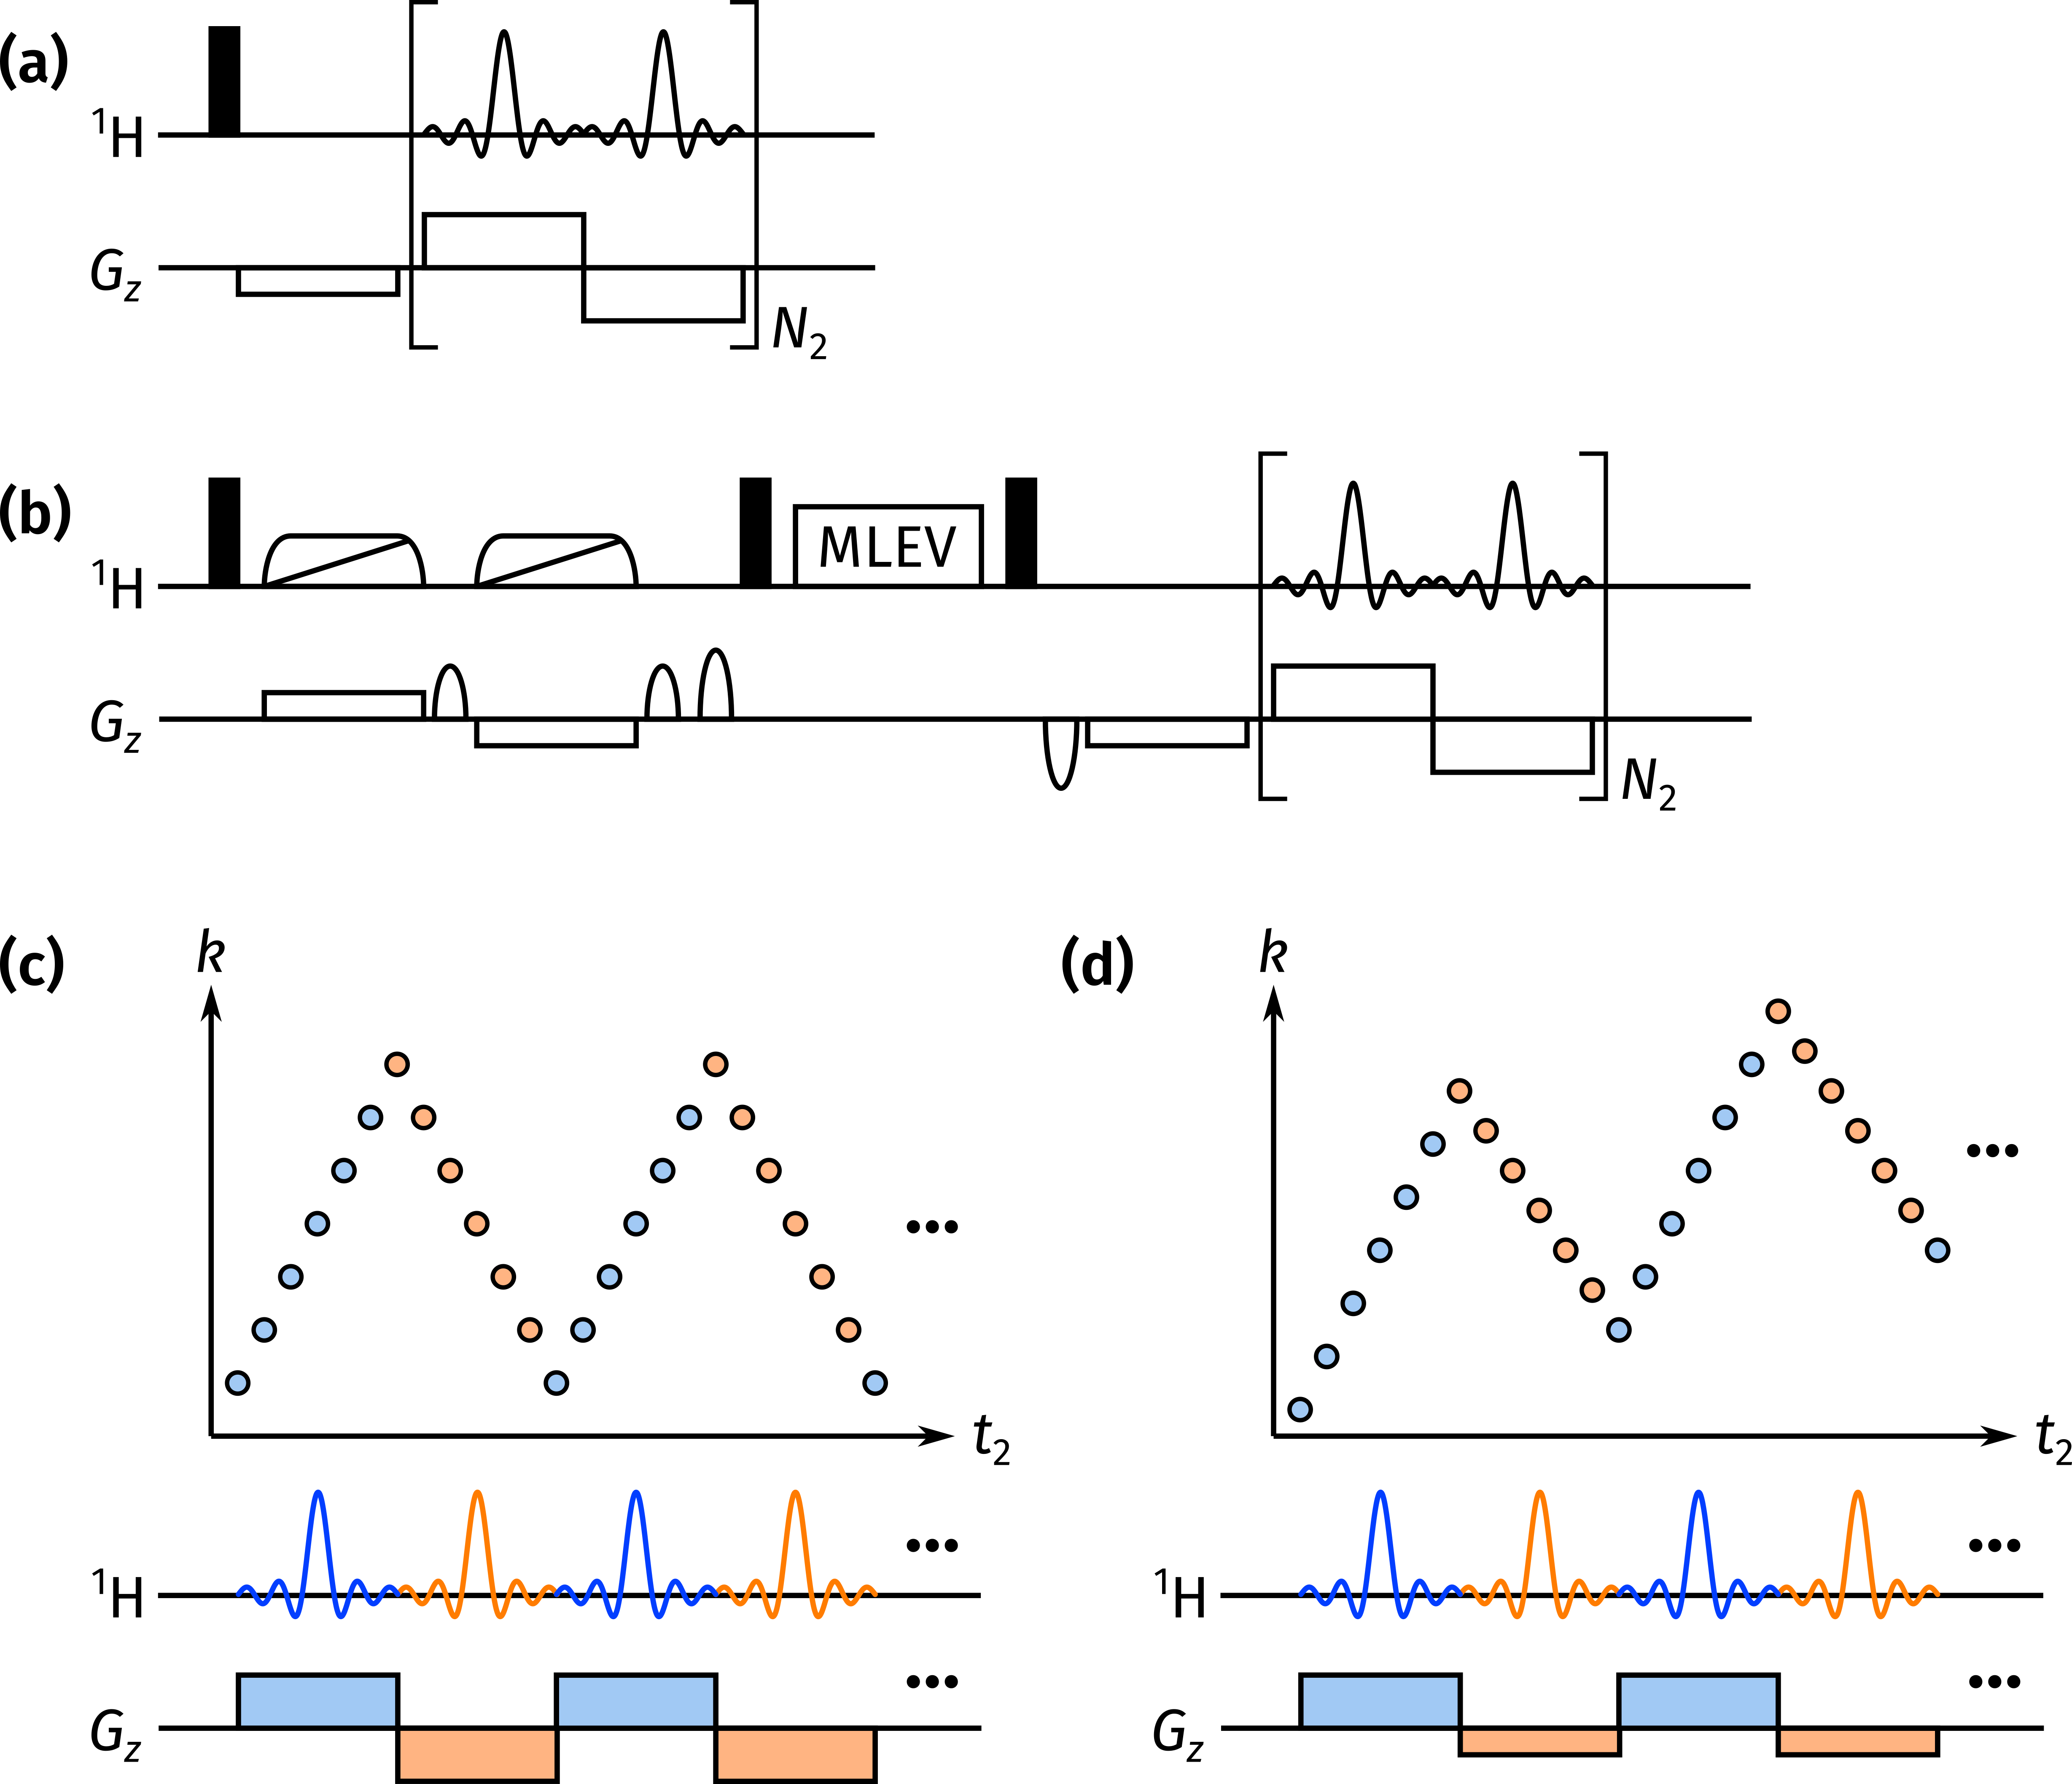
\includegraphics[]{pp/poise/epsi.png}%
    {\phantomsubcaption\label{fig:poise_epsi_zgepsi}}%
    {\phantomsubcaption\label{fig:poise_epsi_tocsyepsi}}%
    {\phantomsubcaption\label{fig:poise_epsi_epsicorrect}}%
    {\phantomsubcaption\label{fig:poise_epsi_epsiwrong}}%
    \caption[Pulse sequences used for EPSI optimisation]{
        Pulse sequences used for EPSI optimisation, and depiction of the $(k, t_2)$ data matrices thus obtained.
        \textbf{(\subref{fig:poise_epsi_zgepsi})} Pulse--EPSI experiment.
        \textbf{(\subref{fig:poise_epsi_tocsyepsi})} Ultrafast TOCSY experiment; gradients were set up according to the protocol of Giraudeau et al.\autocite{Gouilleux2018ARNMRS}
        \textbf{(\subref{fig:poise_epsi_epsicorrect})} Illustration of the $(k, t_2)$ data matrix obtained during an EPSI acquisition period.
        Blue dots indicate data acquired during a positive gradient, and orange dots data acquired during the negative gradient.
        \textbf{(\subref{fig:poise_epsi_epsiwrong})} The $(k, t_2)$ data matrix obtained when the positive and negative EPSI gradients (blue and orange in the pulse sequences) are not balanced.
        In this case, the negative gradient is slightly weaker, leading to a `drift' towards larger values of $k$.
    }
    \label{fig:poise_epsi}
\end{figure}

During an EPSI acquisition period, alternating gradients of equal magnitude but opposite sign are applied, as shown in \cref{fig:poise_epsi_zgepsi,fig:poise_epsi_tocsyepsi}. Each data point collected therefore depends not only on $t_2$ (the acquisition time domain) but also on $k$, a wavenumber which measures the extent of gradient dephasing caused by the acquisition gradients:
\begin{equation}
    \label{eq:epsi_k_space}
    k = \int_0^{t_2} \gamma G(t) \,\mathrm{d}t.
\end{equation}
This value of $k$ increases during positive gradients and decreases during negative gradients, leading to a zigzag pattern in $k$-space, all while $t_2$ is still increasing (\cref{fig:poise_epsi_epsicorrect}).
The \textit{prephasing gradient} immediately before acquisition has the same duration as the EPSI gradients, but has half the amplitude, meaning that $k$ begins from a negative value, specifically, $k_\text{max} / 2$, where $k_\text{max}$ is the change in $k$ caused by one complete positive EPSI gradient.
As explained in previous reviews\autocite{Frydman2003JACS}, the spatial profile $f(z)$ can be obtained by Fourier transformation of the $k$ domain.
Alternatively, since $t_1$ is proportional to $z$ and the indirect-dimension frequency $F_1$ is itself obtained through Fourier transformation of the $t_1$-domain, the $F_1$ and $k$ domains are in fact directly proportional: no Fourier transform is required along this axis to obtain the indirect-dimension frequencies.

This rapid alternating of gradients is very demanding on spectrometers, and it is often the case that the positive and negative EPSI gradients---although \textit{nominally} specified with the same amplitude---are not perfectly balanced.
This causes a `drift' in the $k$-domain over time, as illustrated in \cref{fig:poise_epsi_epsiwrong}.
In this section, POISE is used to perform an \textit{instrument-specific} optimisation in order to correct for this effect.


\subsubsection{Optimisation setup}

To measure the drift in $k$-space, it is easiest to use a pulse sequence for which there is no spatial encoding; the pulse--EPSI experiment (\cref{fig:poise_epsi_zgepsi}) is perfectly suited for this.
In the pulse programme, I multiplied the amplitudes of the negative gradients by a factor $\alpha$, represented as \texttt{CNST16} in TopSpin:
the objective of POISE is therefore to determine the optimum value for this which minimises the drift.
Calculating this drift requires fairly substantial processing, which is most easily done inside the cost function using \texttt{numpy} functions (rather than, for example, a TopSpin AU script).
The \texttt{epsi\_gradient\_drift} cost function therefore consists of the following steps:
\begin{enumerate}
    \item reading in the 1D FID and reshaping it into a 2D $(k, t_2)$ matrix;
    \item discarding data obtained during negative gradients;
    \item determining, for each point in $t_2$, the value of $k$ for which the maximum signal is found;
    \item performing linear regression on these points and obtaining the slope of $k$ against $t_2$, the absolute value of which directly represents the extent of $k$-space drifting.
\end{enumerate}

\begin{figure}[htb]
    \centering
    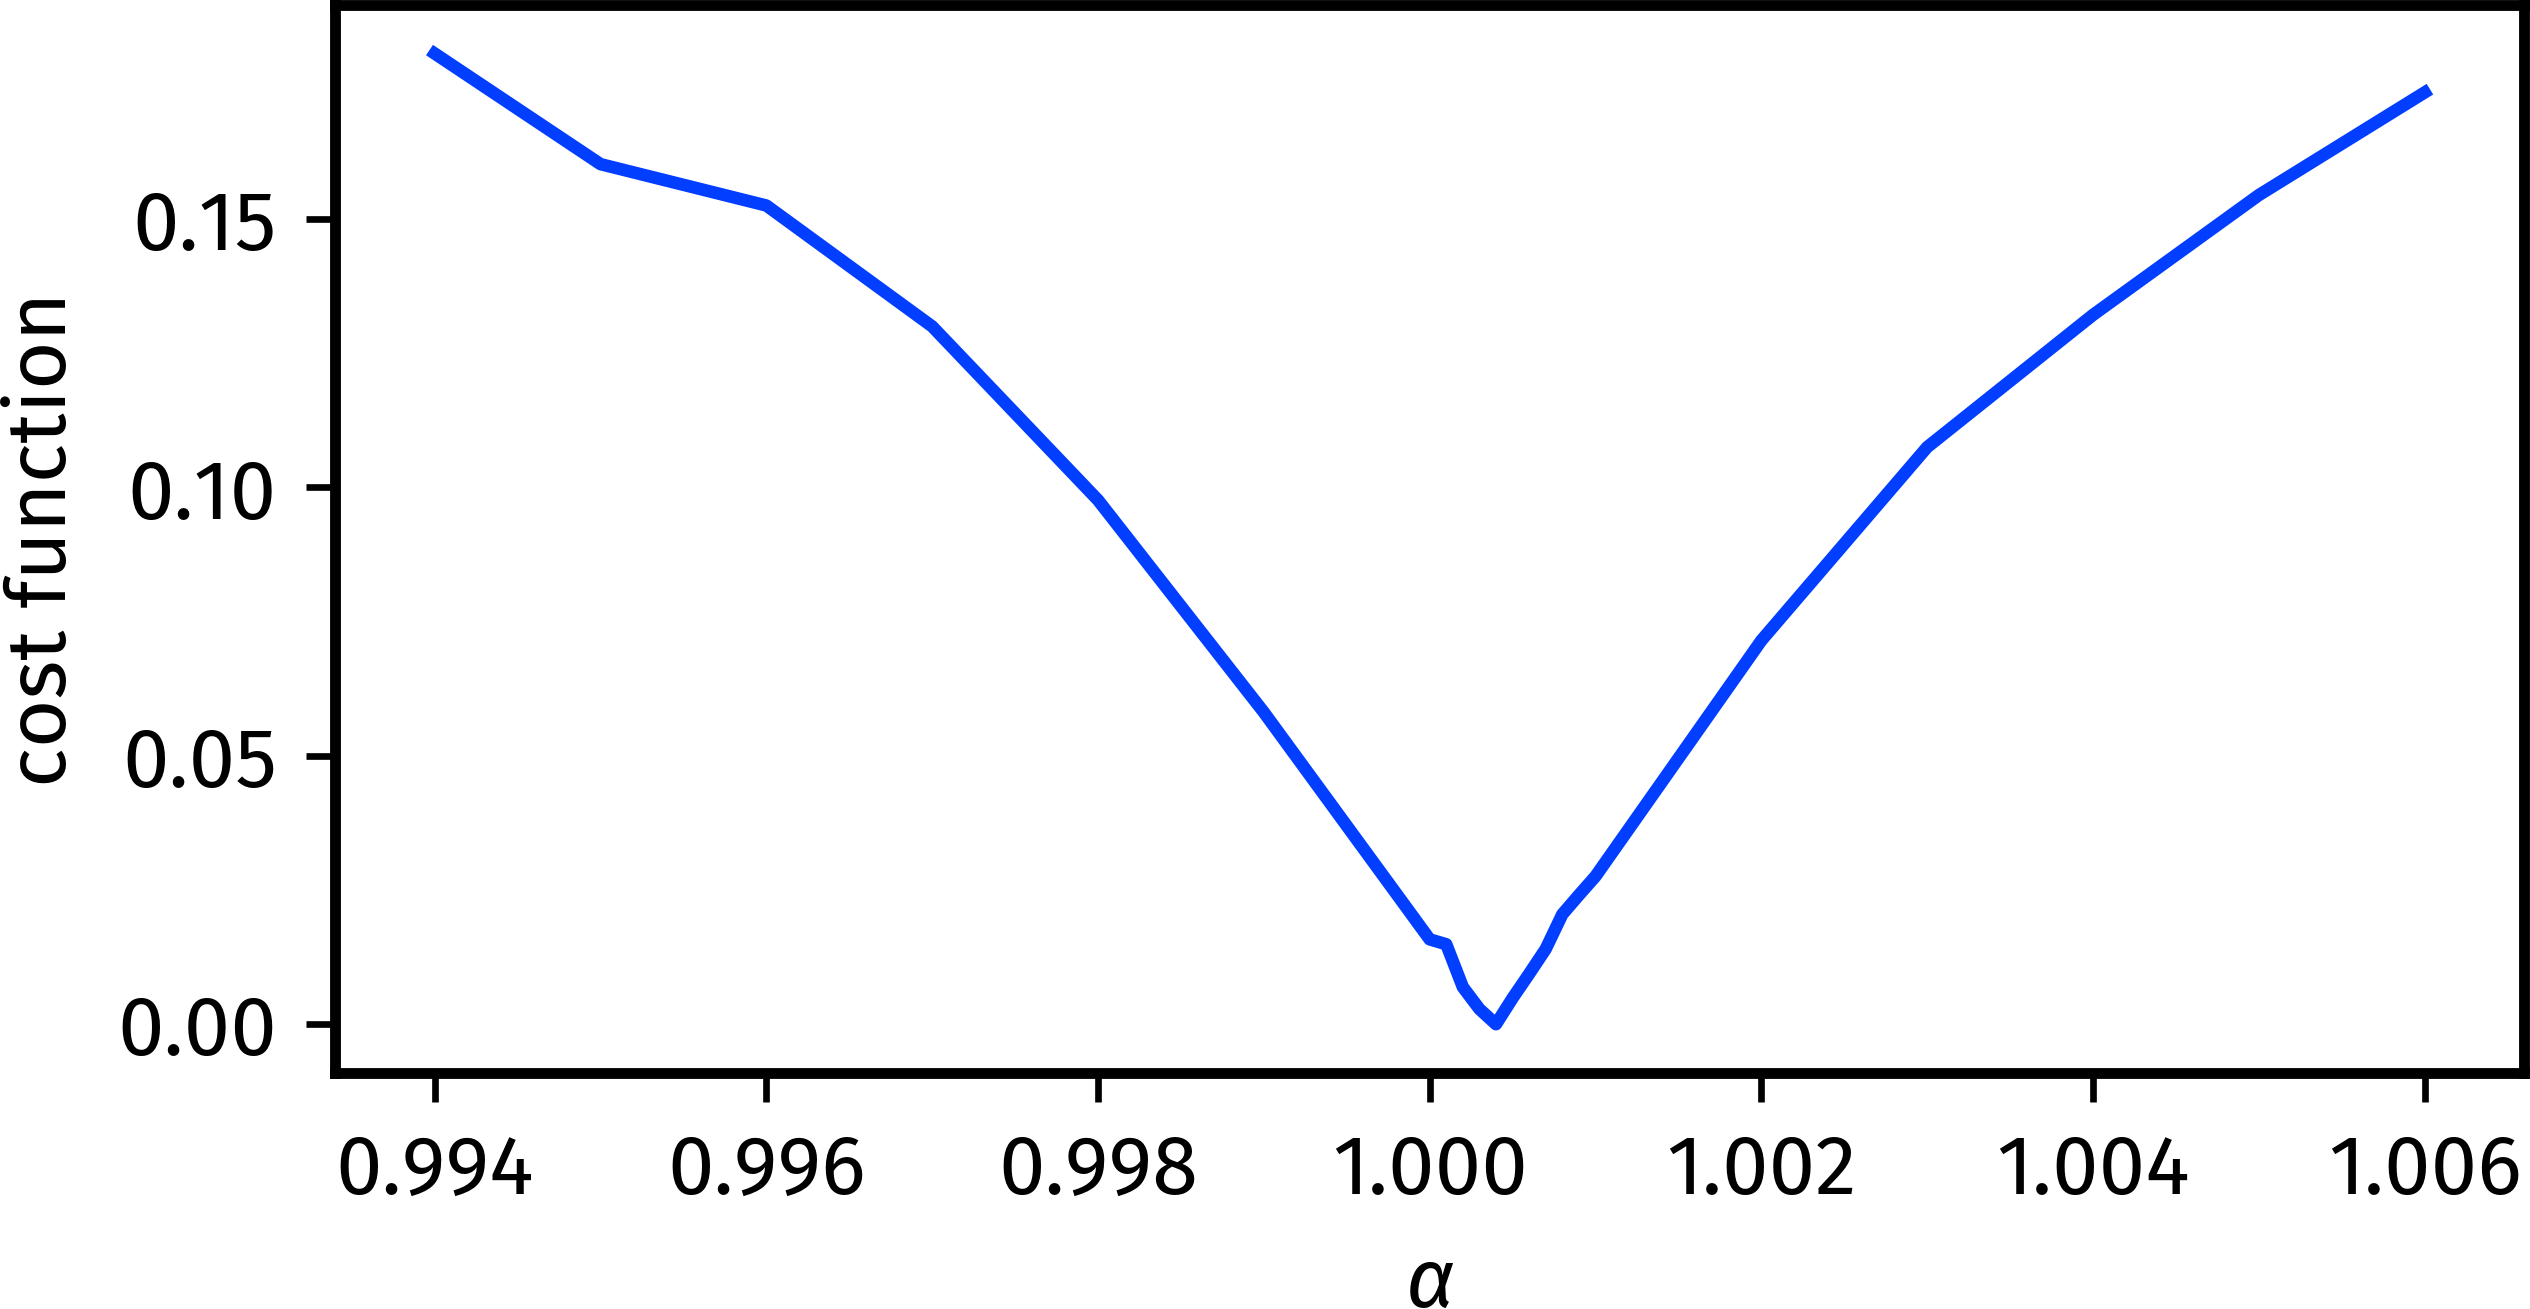
\includegraphics[]{figures/poise/epsi_scan.png}%
    \caption[Reference grid search for EPSI optimisation]{
        Reference grid search for EPSI optimisation.
        \datacode{6F-210316}
    }
    \label{fig:poise_epsi_scan}
\end{figure}

Since the cost function constructed here was relatively complicated, I carried out a reference grid search to confirm that it was working as intended (\cref{fig:poise_epsi_scan}).
This yielded an expected optimum of $\alpha = 1.0004$.
(The sample used here was ferulic acid, but in principle this should not matter as the drift is due to the spectrometer and not the sample.)

To save time in the optimisation itself, I reused the strategy of setting \texttt{DS=0} and \texttt{NS=1}.
As before, since each FE is separated by approximately five seconds of processing and spectrometer initialisation, this means that there is no need for another recovery delay; thus, \texttt{D1} was set to \qty{0.5}{\s}.
However, note that such a short recovery delay should \textit{not} be used if \texttt{DS} is larger than 0 or \texttt{NS} larger than 1: EPSI acquisitions should not be carried out in rapid succession.
Furthermore, \texttt{AQ} should be kept under \qty{100}{\ms}.


\subsubsection{Optimisation results}

\begin{table}[htb]
    \hbadness=10000
    \centering
    \begin{tabular}{ccccc}
        \toprule
        Entry & Algorithm & Optimum found      & FEs & Time taken (\unit{\s}) \\
        \midrule
        1     & NM        & 1.000375           & 10  & 49--52               \\
        2     & MDS       & 1.000375           & 10  & 49--50               \\
        3     & BOBYQA    & 1.000383--1.000388 & 7   & 34--35               \\
        \bottomrule
    \end{tabular}
    \caption[EPSI gradient imbalance optimisations]{
        Results of EPSI gradient imbalance optimisations.
        Note that in practice, all of these optimisations actually converge to $\alpha = 1.0004$; the extra decimal place is not used by the spectrometer (see text for further discussion).
        The POISE routine used here is: \mintinline[breaklines]{json}{{"name": "epsi", "pars": ["cnst16"], "lb": [0.99], "ub": [1.01], "init": [1.0], "tol": [0.0001], "cf": "epsi_gradient_drift", "au": "poise_1d"}}.
        \datacode{6F-210316}
    }
    \label{tbl:poise_epsi}
\end{table}

In the event, all three optimisation algorithms successfully find the the optimal value of $\alpha$ in under a minute (\cref{tbl:poise_epsi}).
It is worth clarifying one subtlety of POISE here.
In the table, the optima are quoted to a rather greater precision than one might expect at first: however, the actual precision of the optimisation result is not given by the number of significant figures,\footnote{The entire concept of `significant figures' is a very crude way of expressing uncertainty anyway.} but rather a combination of two factors:

\begin{itemize}
    \item first, the \textit{optimisation tolerance}, which is purely determined by the optimisation routine. Thus, in \cref{tbl:poise_epsi}, the optimum of 1.000375 actually means $1.000375 \pm 0.0001$ (and not $1.000375 \pm 0.0000005$, as `significant figures' would imply); and
    \item second, the available \textit{spectrometer resolution}, which represents how precisely the spectrometer can implement a given parameter value.
        In this case, the available resolution is $0.0001$, which means that even if we input the `optimum' of $\alpha = 1.000375$, the experiment is executed with $\alpha = 1.0004$ (see also \cref{fig:epsi_spec}).
        The optimisation algorithm has no knowledge of this, so it still reports a value of $1.000375$.
        When reporting optima from POISE, users should be wary of this.
\end{itemize}

This further underlines the importance of choosing a sensible optimisation tolerance: it should be \textit{at least} as large as the instrument resolution (larger values can be used when an extremely accurate result is not needed).

\begin{figure}[htb]
    \centering
    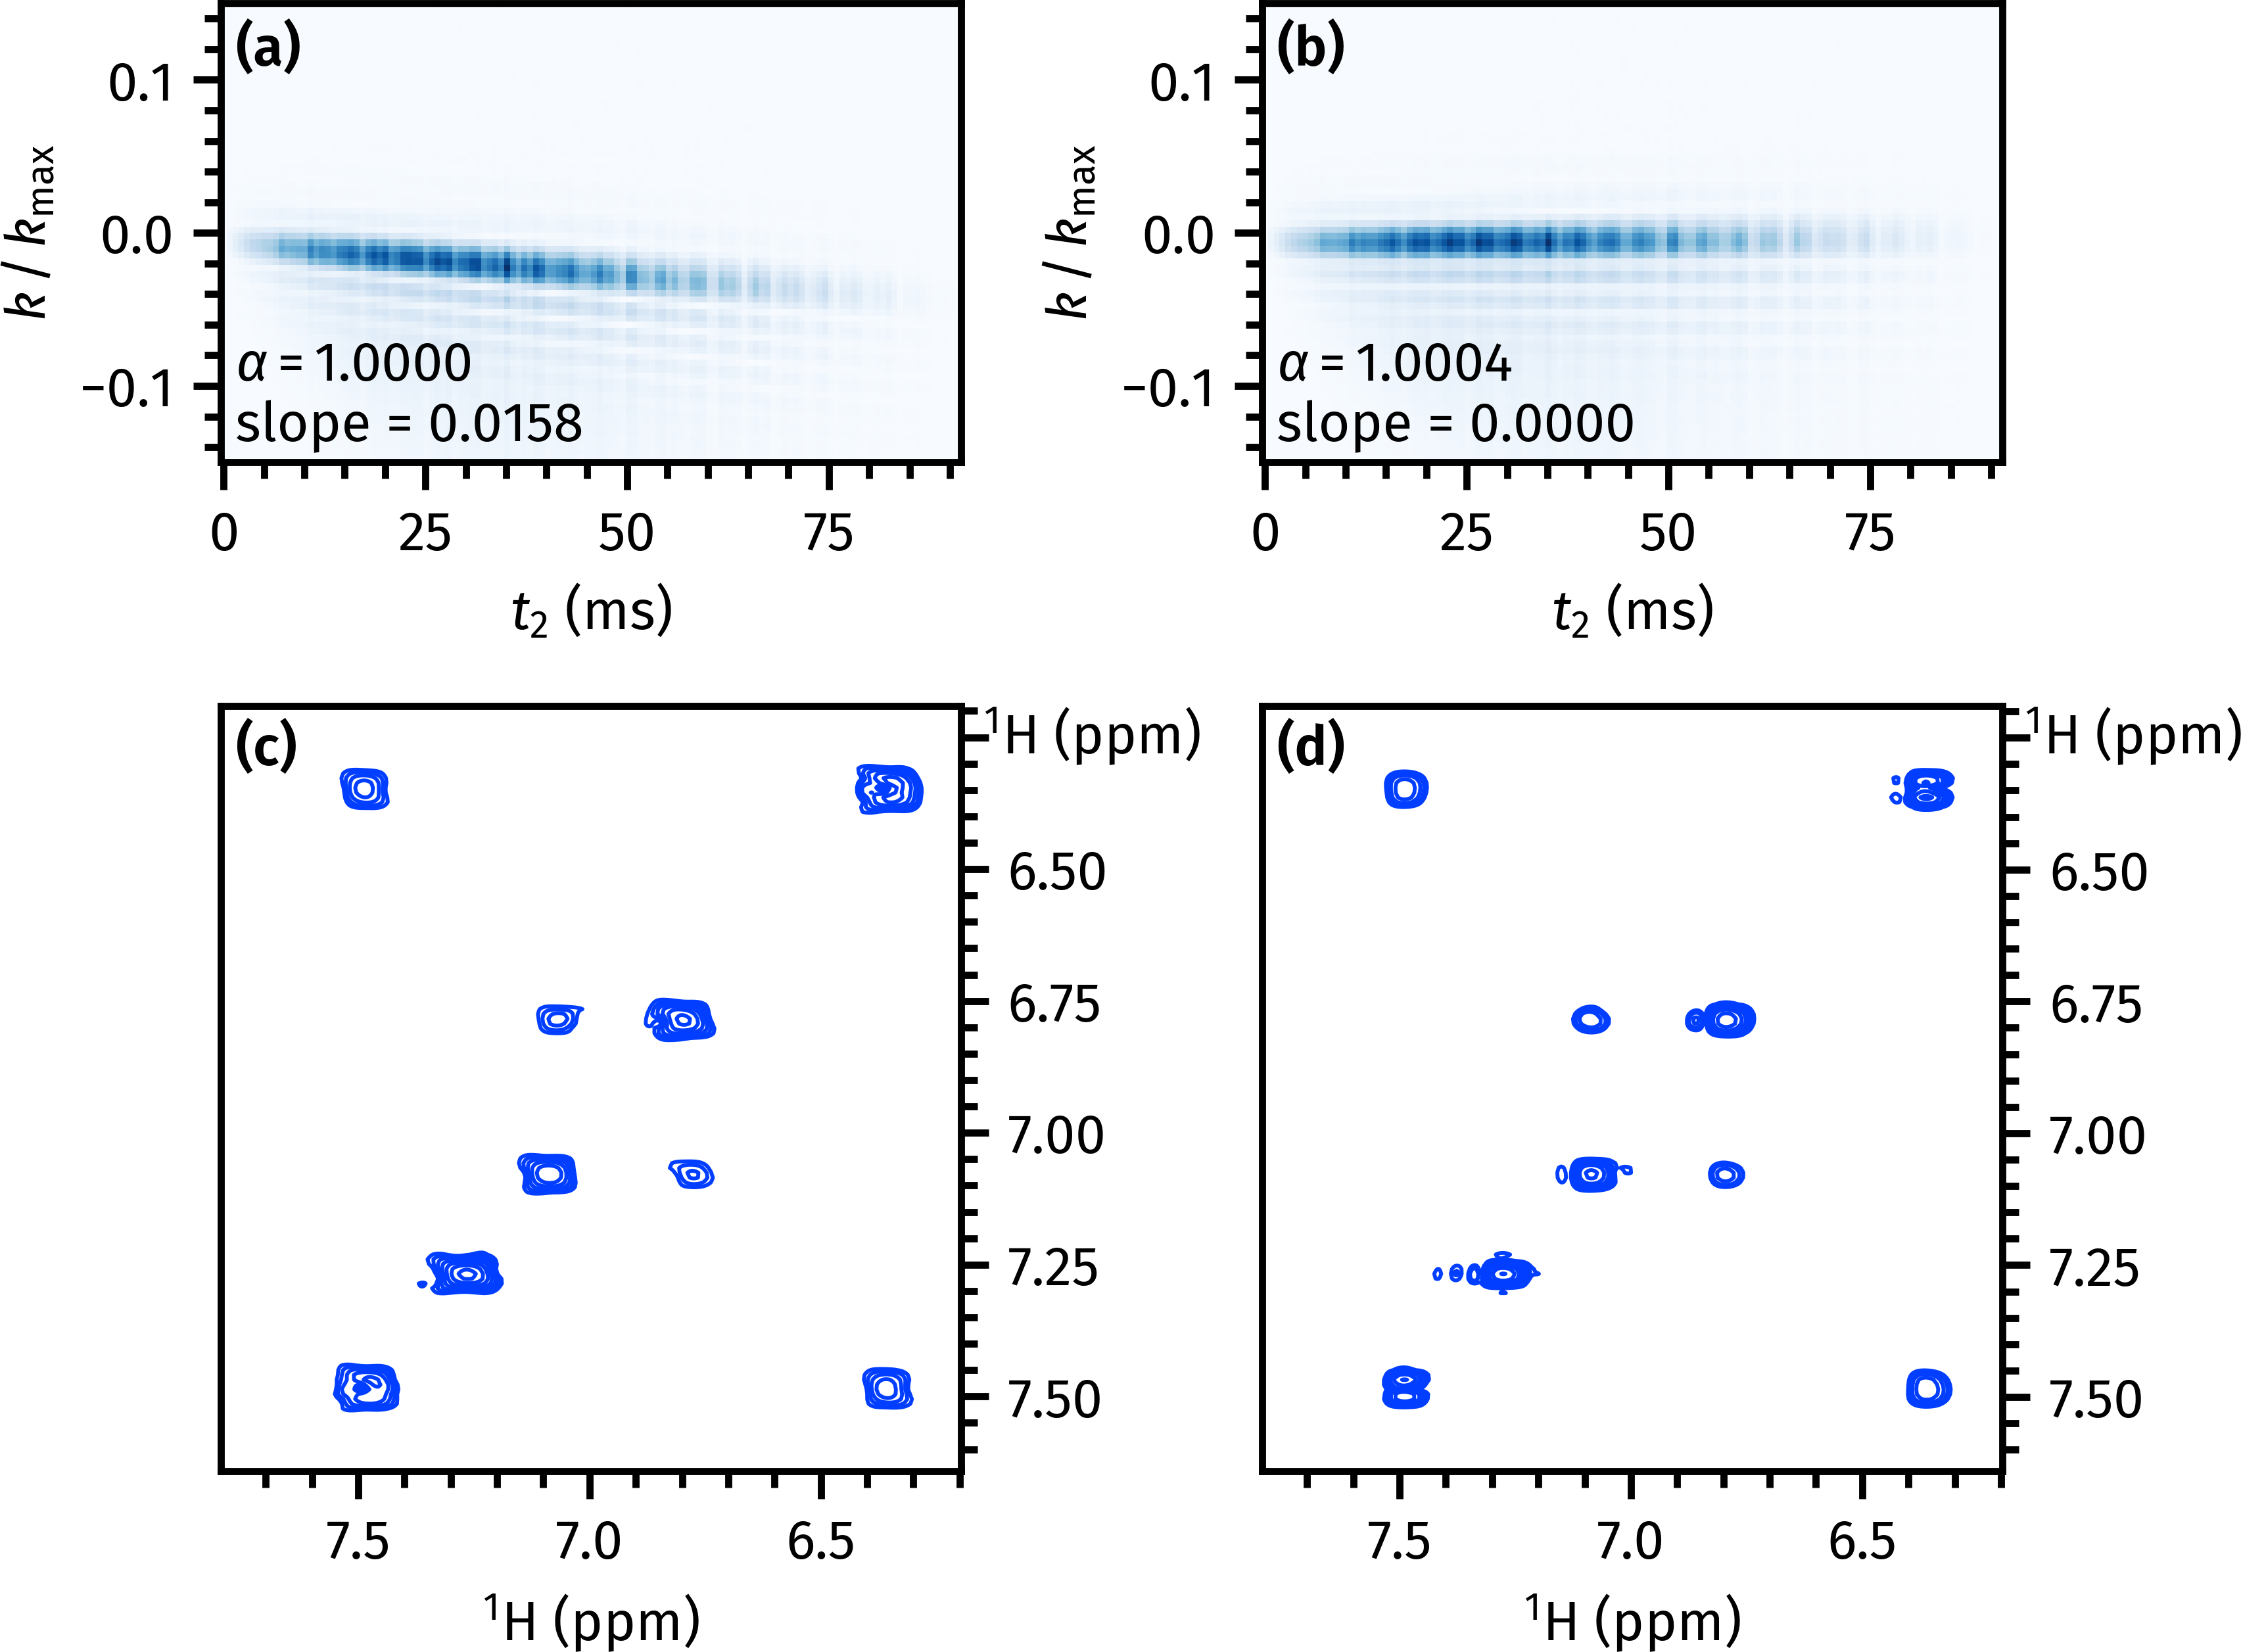
\includegraphics[]{poise/epsi_spec.png}%
    {\phantomsubcaption\label{fig:epsi_spec_kt_noopt}}%
    {\phantomsubcaption\label{fig:epsi_spec_kt_opt}}%
    {\phantomsubcaption\label{fig:epsi_spec_tocsy_noopt}}%
    {\phantomsubcaption\label{fig:epsi_spec_tocsy_opt}}%
    \caption[Comparison between unoptimised and optimised EPSI spectra]{
        \textbf{(\subref{fig:epsi_spec_kt_noopt},\subref{fig:epsi_spec_kt_opt})} Magnitude-mode $(k, t_2)$ data matrices obtained from the pulse--EPSI experiment, before and after optimisation of $\alpha$ respectively.
        \textbf{(\subref{fig:epsi_spec_tocsy_noopt},\subref{fig:epsi_spec_tocsy_opt})} The corresponding 2D ultrafast TOCSY spectra, recorded with the unoptimised and optimised value of $\alpha$ respectively.
        The MLEV mixing period used was \qty{10}{\ms}.
    }
    \label{fig:epsi_spec}
\end{figure}

The $(k, t_2)$ data matrices obtained from the excitation--EPSI pulse sequence are shown in \cref{fig:epsi_spec_kt_noopt,fig:epsi_spec_kt_opt}.
In the former, where the default value of $\alpha = 1$ is used, there is a noticeable drift in $k$-space.
This is removed in the optimised experiment with $\alpha = 1.0004$.
Using the optimised value of $\alpha$ in fact leads to much improved ultrafast spectra, such as the TOCSY spectra recorded with the pulse sequence in \cref{fig:poise_epsi_tocsyepsi}.
\Cref{fig:epsi_spec_tocsy_noopt,fig:epsi_spec_tocsy_opt} show respectively the ultrafast TOCSY spectra recorded without and with optimisation of the gradient ratio $\alpha$.
In the latter, substantial improvements in lineshapes are obtained, even allowing some couplings to be properly resolved in the indirect dimension.
In principle, this $k$-drift could be compensated for by shearing of the $(k, t_2)$ data matrix prior to Fourier transformation.
However, similar improvements in lineshapes could not be accomplished using the \texttt{ufproc.py} processing script provided by Giraudeau et al.\autocite{Gouilleux2018ARNMRS} (and I did not attempt to do so manually).

\subsection{HMBC low-pass J-filter}
\label{subsec:poise__hmbc}

In this and the remaining examples, we look at optimisations involving \textit{multiple parameters}, one of the key strengths of POISE.
Grid searches are extremely ineffective for this purpose, as the number of FEs required scales exponentially with the number of parameters; human trial-and-error can also be very difficult as parameters may be tightly \textit{coupled}, meaning that the optimum cannot simply be found by optimising one parameter at a time.
In contrast, the optimisation algorithms used in POISE make no assumption about the relationship between the two parameters.
Furthermore, since only local minima are sought, the time required for convergence scales approximately linearly with the number of parameters, at least in the regimes which I have tested.%
\footnote{I am not actually aware of any \textit{theoretical} results which show how the number of function evaluations scales with the number of parameters in an optimisation; I suspect the answer depends on the exact problem being solved.}

\begin{figure}[htb]
    \centering
    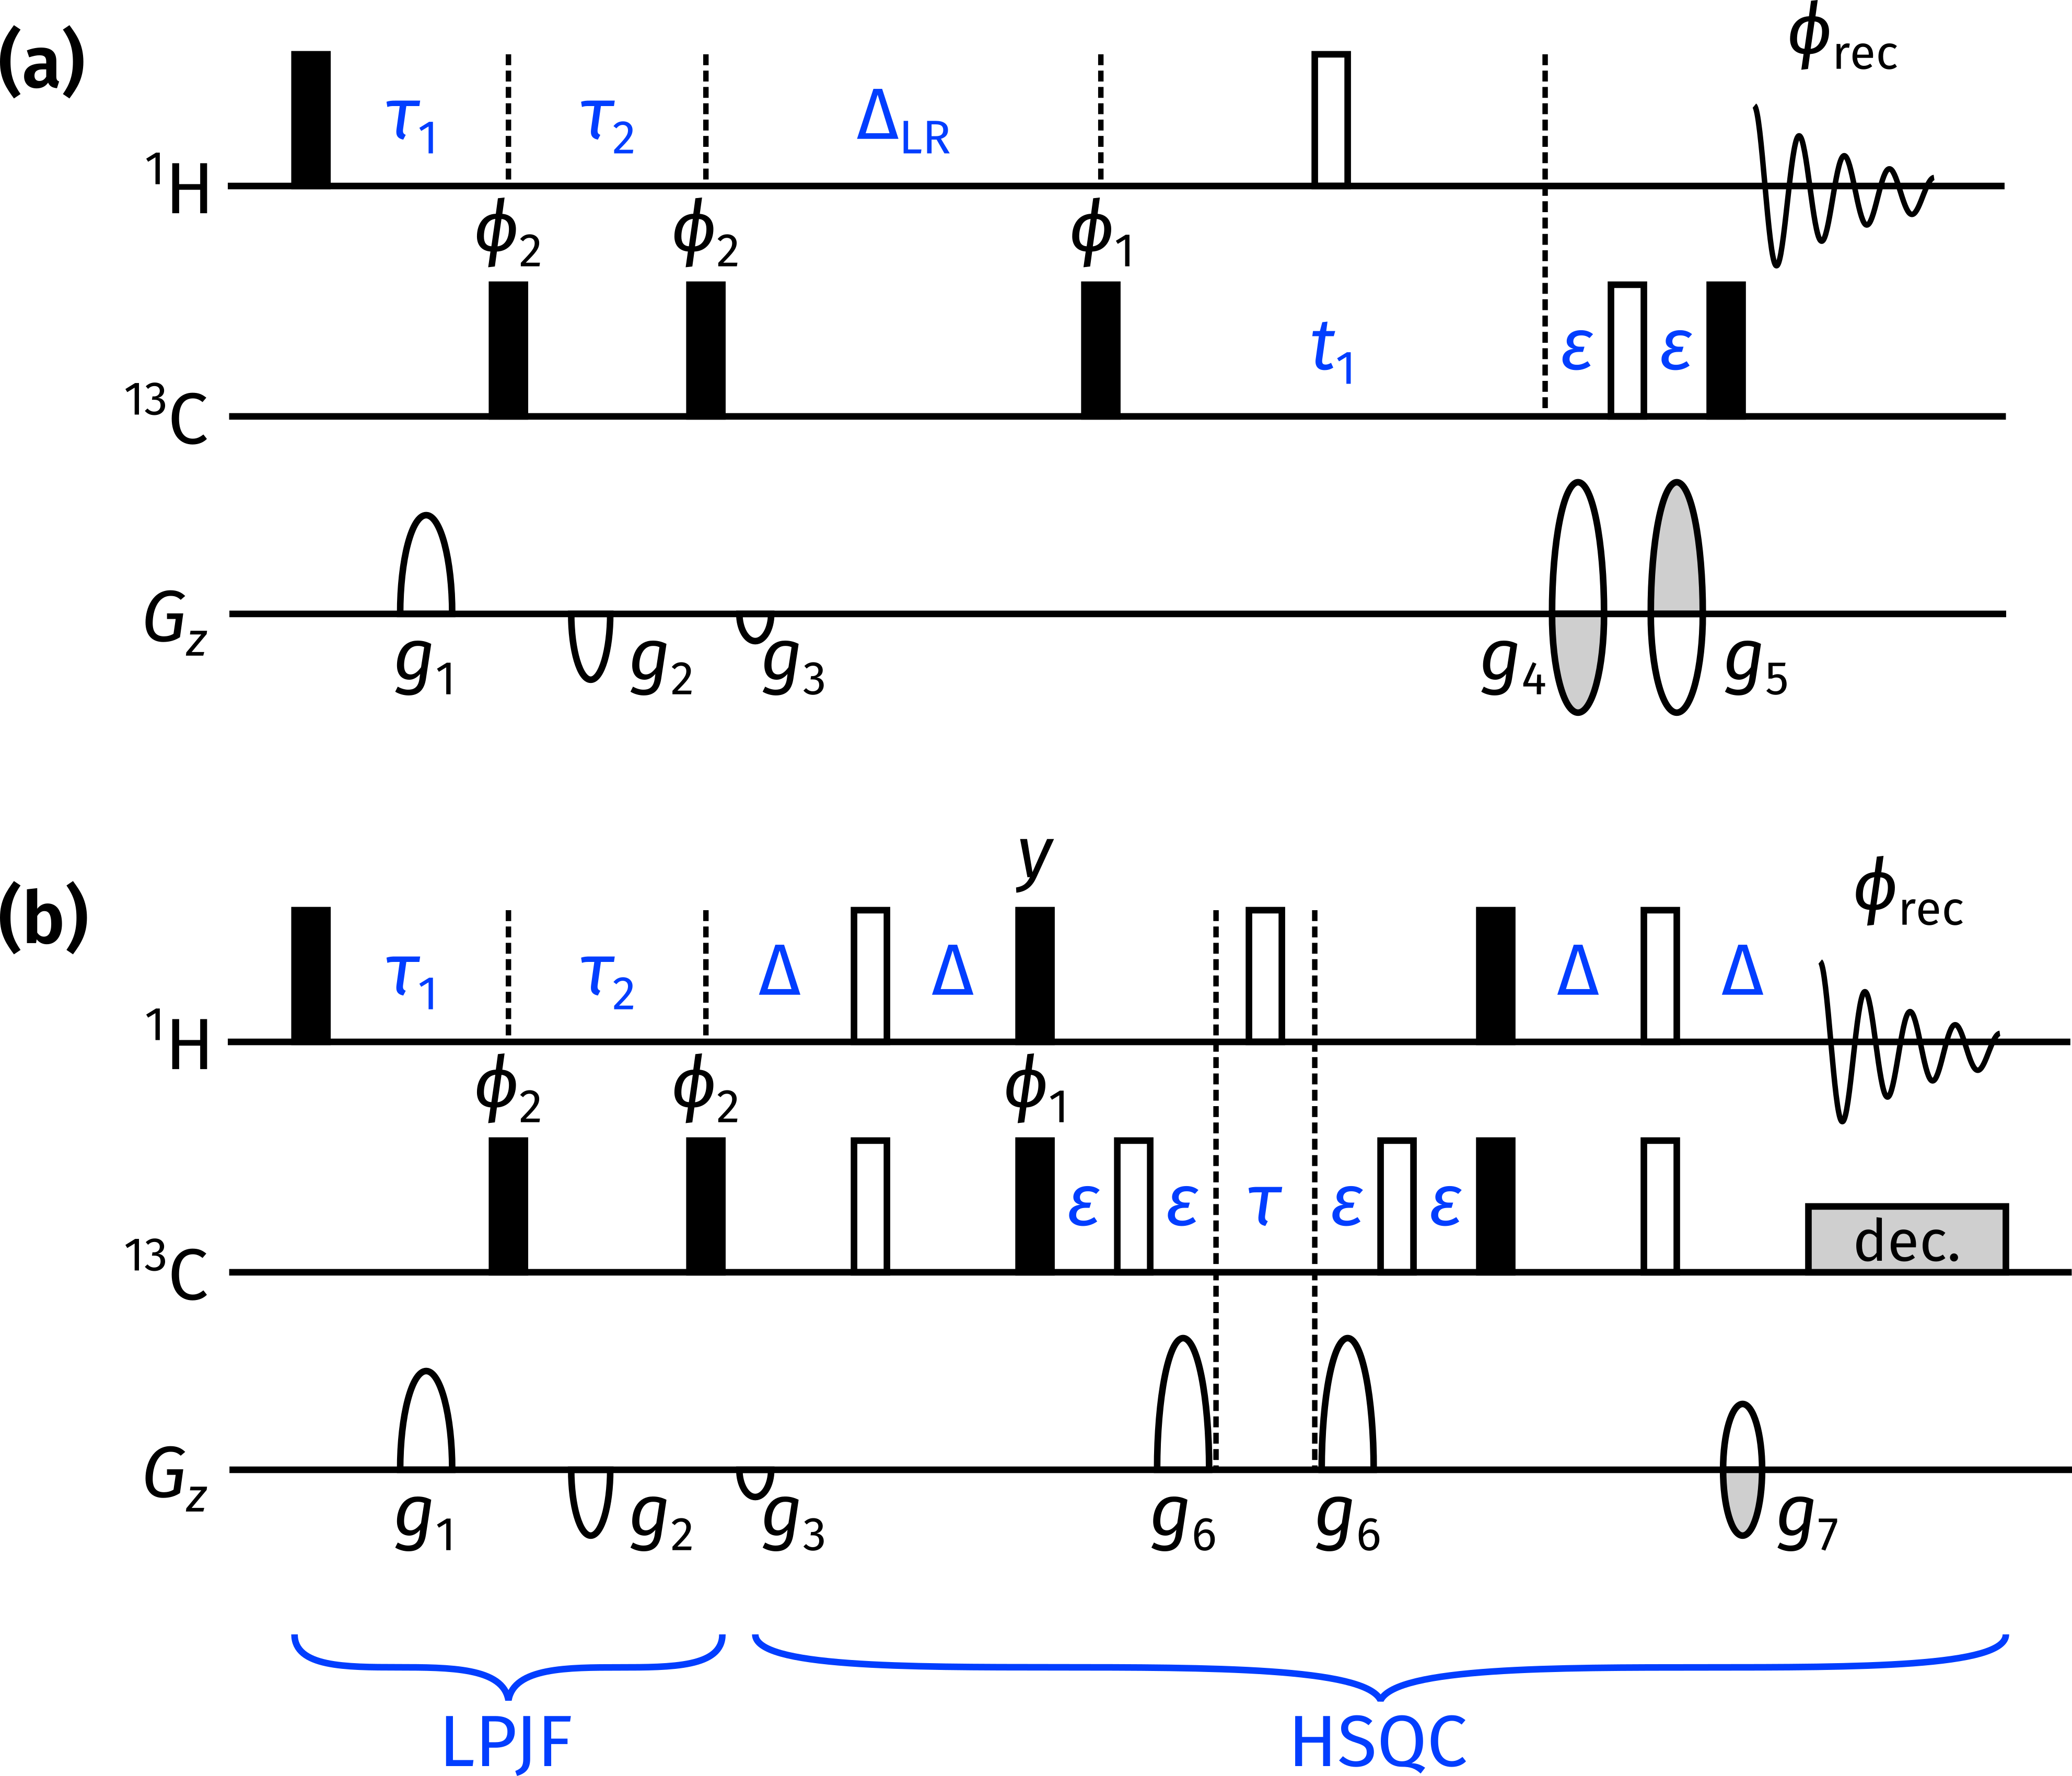
\includegraphics[]{pp/poise/hmbc.png}%
    {\phantomsubcaption\label{fig:poise_hmbc_pulseq_hmbc}}%
    {\phantomsubcaption\label{fig:poise_hmbc_pulseq_hsqc}}%
    \caption[Pulse sequences used for HMBC optimisation]{
        \textbf{(\subref{fig:poise_hmbc_pulseq_hmbc})} Standard 2D HMBC pulse sequence with a second-order low-pass J-filter.
        \textbf{(\subref{fig:poise_hmbc_pulseq_hsqc})} 1D LPJF--HSQC pulse sequence used in the POISE optimisation.
        In practice, only the first increment of this experiment was recorded.
        Delays are set as follows: $\Delta = 1 / (4 \cdot \oneJ{CH}); \Delta_\text{LR} = 1 / (2 \cdot \nJ{CH})$; $\tau$ is as short as possible (several microseconds); and $\tau_1$ and $\tau_2$ are as described in the text.
        Phase cycling is performed with $\phi_1 = \phi_\text{rec} = (x, -x)$, and $\phi_2 = (x, x, -x, -x)$.
        Gradient amplitudes are: $(g_1, g_2, g_3) = (15\%, -10\%, -5\%)$ for the LPJF, $(g_4, g_5) = (80\%, -47.85\%)$ (or vice versa) for EA selection in the HMBC experiment\autocite{Cicero2001JMR}, and $(g_6, g_7) = (70\%, \pm 35.21\%)$ for EA selection in the LPJF--HSQC experiment.
    }
    \label{fig:poise_hmbc_pulseq}
\end{figure}

In the simplest example of a multiple-parameter optimisation, I use POISE to search for the best delays in the low-pass J-filter (LPJF) of a HMBC experiment (\cref{fig:poise_hmbc_pulseq_hmbc}).
Specifically, a second-order LPJF is used, which has the form $\tau_1$--\ang{90}(\carbon{})--$\tau_2$--\ang{90}(\carbon{}).
The role of the LPJF is to destroy \magn{C} magnetisation at the start of the HMBC, which would otherwise generate one-bond artefacts in the resulting spectrum (essentially HSQC signals, but coupled in $F_2$).
Assuming that the $\oneJ{CH}$ values span a range of $J_\text{min}$ to $J_\text{max}$, S{\o}rensen and coworkers have provided `theoretical' best values for the delays:\autocite{Nielsen1986JMR,Meissner2000MRC}
\begin{align}
    \tau_1 &= \frac{1}{2} [J_\text{min} + 0.146(J_\text{max} - J_\text{min})]^{-1}; \label{eq:hmbc_lpjf_theoretical_min} \\
    \tau_2 &= \frac{1}{2} [J_\text{max} - 0.146(J_\text{max} - J_\text{min})]^{-1}. \label{eq:hmbc_lpjf_theoretical_max}
\end{align}
In practice, the TopSpin standard library HMBC sequence (\texttt{hmbcetgpl2nd}) uses delays of
\begin{equation}
    \tau_1 = \frac{1}{2J_\text{min}}; \quad \tau_2 = \frac{1}{2J_\text{max}}. \label{eq:hmbc_lpjf_bruker}
\end{equation}
In either case, though, these delays neglect the actual \textit{distribution} of $\oneJ{CH}$: if many of the couplings are clustered around one particular value, then adjusting the delays to better suppress these values will yield better results.
(Since $\oneJ{CH}$ roughly correlates with the hybridisation of the \carbon{} atom,\autocite{Krivdin2018PNMRS} this can easily happen, for example, if the molecule is predominantly aliphatic or predominantly aromatic.)


\subsubsection{Optimisation setup}

In order for the optimisation routine to minimise the artefacts, it must first have a cost function which can measure the extent of these artefacts.
Given a full 2D HMBC spectrum, it is very difficult to discern which of the peaks are indeed artefacts (of course, this is exactly why it is worthwhile to suppress them).
However, by using a specially designed LPJF--HSQC experiment (\cref{fig:poise_hmbc_pulseq_hsqc}), the artefacts can be isolated without any of the HMBC signals appearing:
this works because any \magn{C} magnetisation which is \textit{not} destroyed by the LPJF will be sampled in the HSQC segment which follows.
Although the LPJF--HSQC can in principle be recorded as a full 2D experiment, to save time, I chose to only record the first increment as a 1D experiment.
\carbon{} decoupling is not mandatory, but the boost in SNR shortens the time needed for optimisation and also reduces noise in the cost function.

For simplicity, I chose to reuse the definitions of $\tau_1$ and $\tau_2$ in the Bruker library sequence (\cref{eq:hmbc_lpjf_bruker}): the optimisation parameters are $J_\text{min}$ and $J_\text{max}$.%
\footnote{Note that using the definitions in \cref{eq:hmbc_lpjf_theoretical_min,eq:hmbc_lpjf_theoretical_max} would not yield any difference in the final optimised result, since it is always possible to tweak $J_\text{min}$ and $J_\text{max}$ in \cref{eq:hmbc_lpjf_bruker} to match these `better' values of $\tau_1$ and $\tau_2$.}
Both parameters were constrained to lie between 100 and \SI{200}{\Hz}, with a tolerance of \SI{3}{\Hz}.
To match the magnitude-mode processing typically used for 2D HMBC experiments, the acquisition AU programme was modified to also process this spectrum in magnitude mode.
The integral of the entire spectrum can therefore be used as the desired cost function for the POISE optimisation.
More specifically, I chose to use a sum of squares:
\begin{equation}
    \label{eq:sos_cost_function}
    f_\text{sos} = \sum_i S_i^2,
\end{equation}
which has the effect of penalising intense artefacts more strongly.


\subsubsection{Optimisation results}

In previous sections, I have quoted ranges for the optima found in an effort to show that the optimisation results are reproducible.
In multiple--parameter optimisations, it is no longer appropriate to report separate ranges for both parameters, since the parameters are in general \textit{interdependent}, in that the spread of values obtained for the first parameter depends on the value obtained for the second, and vice versa.
I therefore only provide ranges for the number of FEs, as well as the time taken.
As for optima found, I will quote only the \textit{best} of these, as measured by the reduction in the cost function.
These optima should therefore not be viewed as a representative summary of the five different runs, but rather as an example of the improvement which may be obtained through POISE.

\begin{table}[htb]
    \hbadness=10000
    \centering
    \begin{tabular}{ccccccc}
        \toprule
              &           & \multicolumn{3}{c}{Best optimum found} & \multicolumn{2}{c}{Aggregated results} \\
        \cmidrule(lr){3-5} \cmidrule(lr){6-7}
        Entry & Algorithm & $J_\text{min}$ & $J_\text{max}$ & $f_\text{sos} / 10^7$ & FEs & Time taken (\si{\s}) \\
        \midrule
        1     & NM        & 143.07 & 185.71                 & 8.65 & 20--24 & 358--430 \\
        2     & MDS       & 141.73 & 185.82                 & 8.36 & 18     & 321--323 \\
        3     & BOBYQA    & 133.38 & 155.03                 & 6.42 & 14--17 & 251--304 \\
        \bottomrule
    \end{tabular}
    \caption[HMBC low-pass J-filter optimisations]{
        Results of HMBC POISE optimisations.
        For each optimisation algorithm, the best optimum found is reported along with the value of the cost function $f_\text{sos}$ (a lower value represents a better optimum).
        The number of FEs, as well as the time taken, is still reported as a range over the five optimisation runs performed per algorithm.
        The POISE routine used here is: \mintinline[breaklines]{json}{{"name": "lpjf", "pars": ["cnst25", "cnst26"], "lb": [100.0, 100.0], "ub": [200.0, 200.0], "init": [120.0, 180.0], "tol": [3.0, 3.0], "cf": "zerorealint_squared", "au": "poise_1d_mc"}}.
        \datacode{7Z-210814}
    }
    \label{tbl:poise_hmbc}
\end{table}

\begin{figure}[htb]
    \centering
    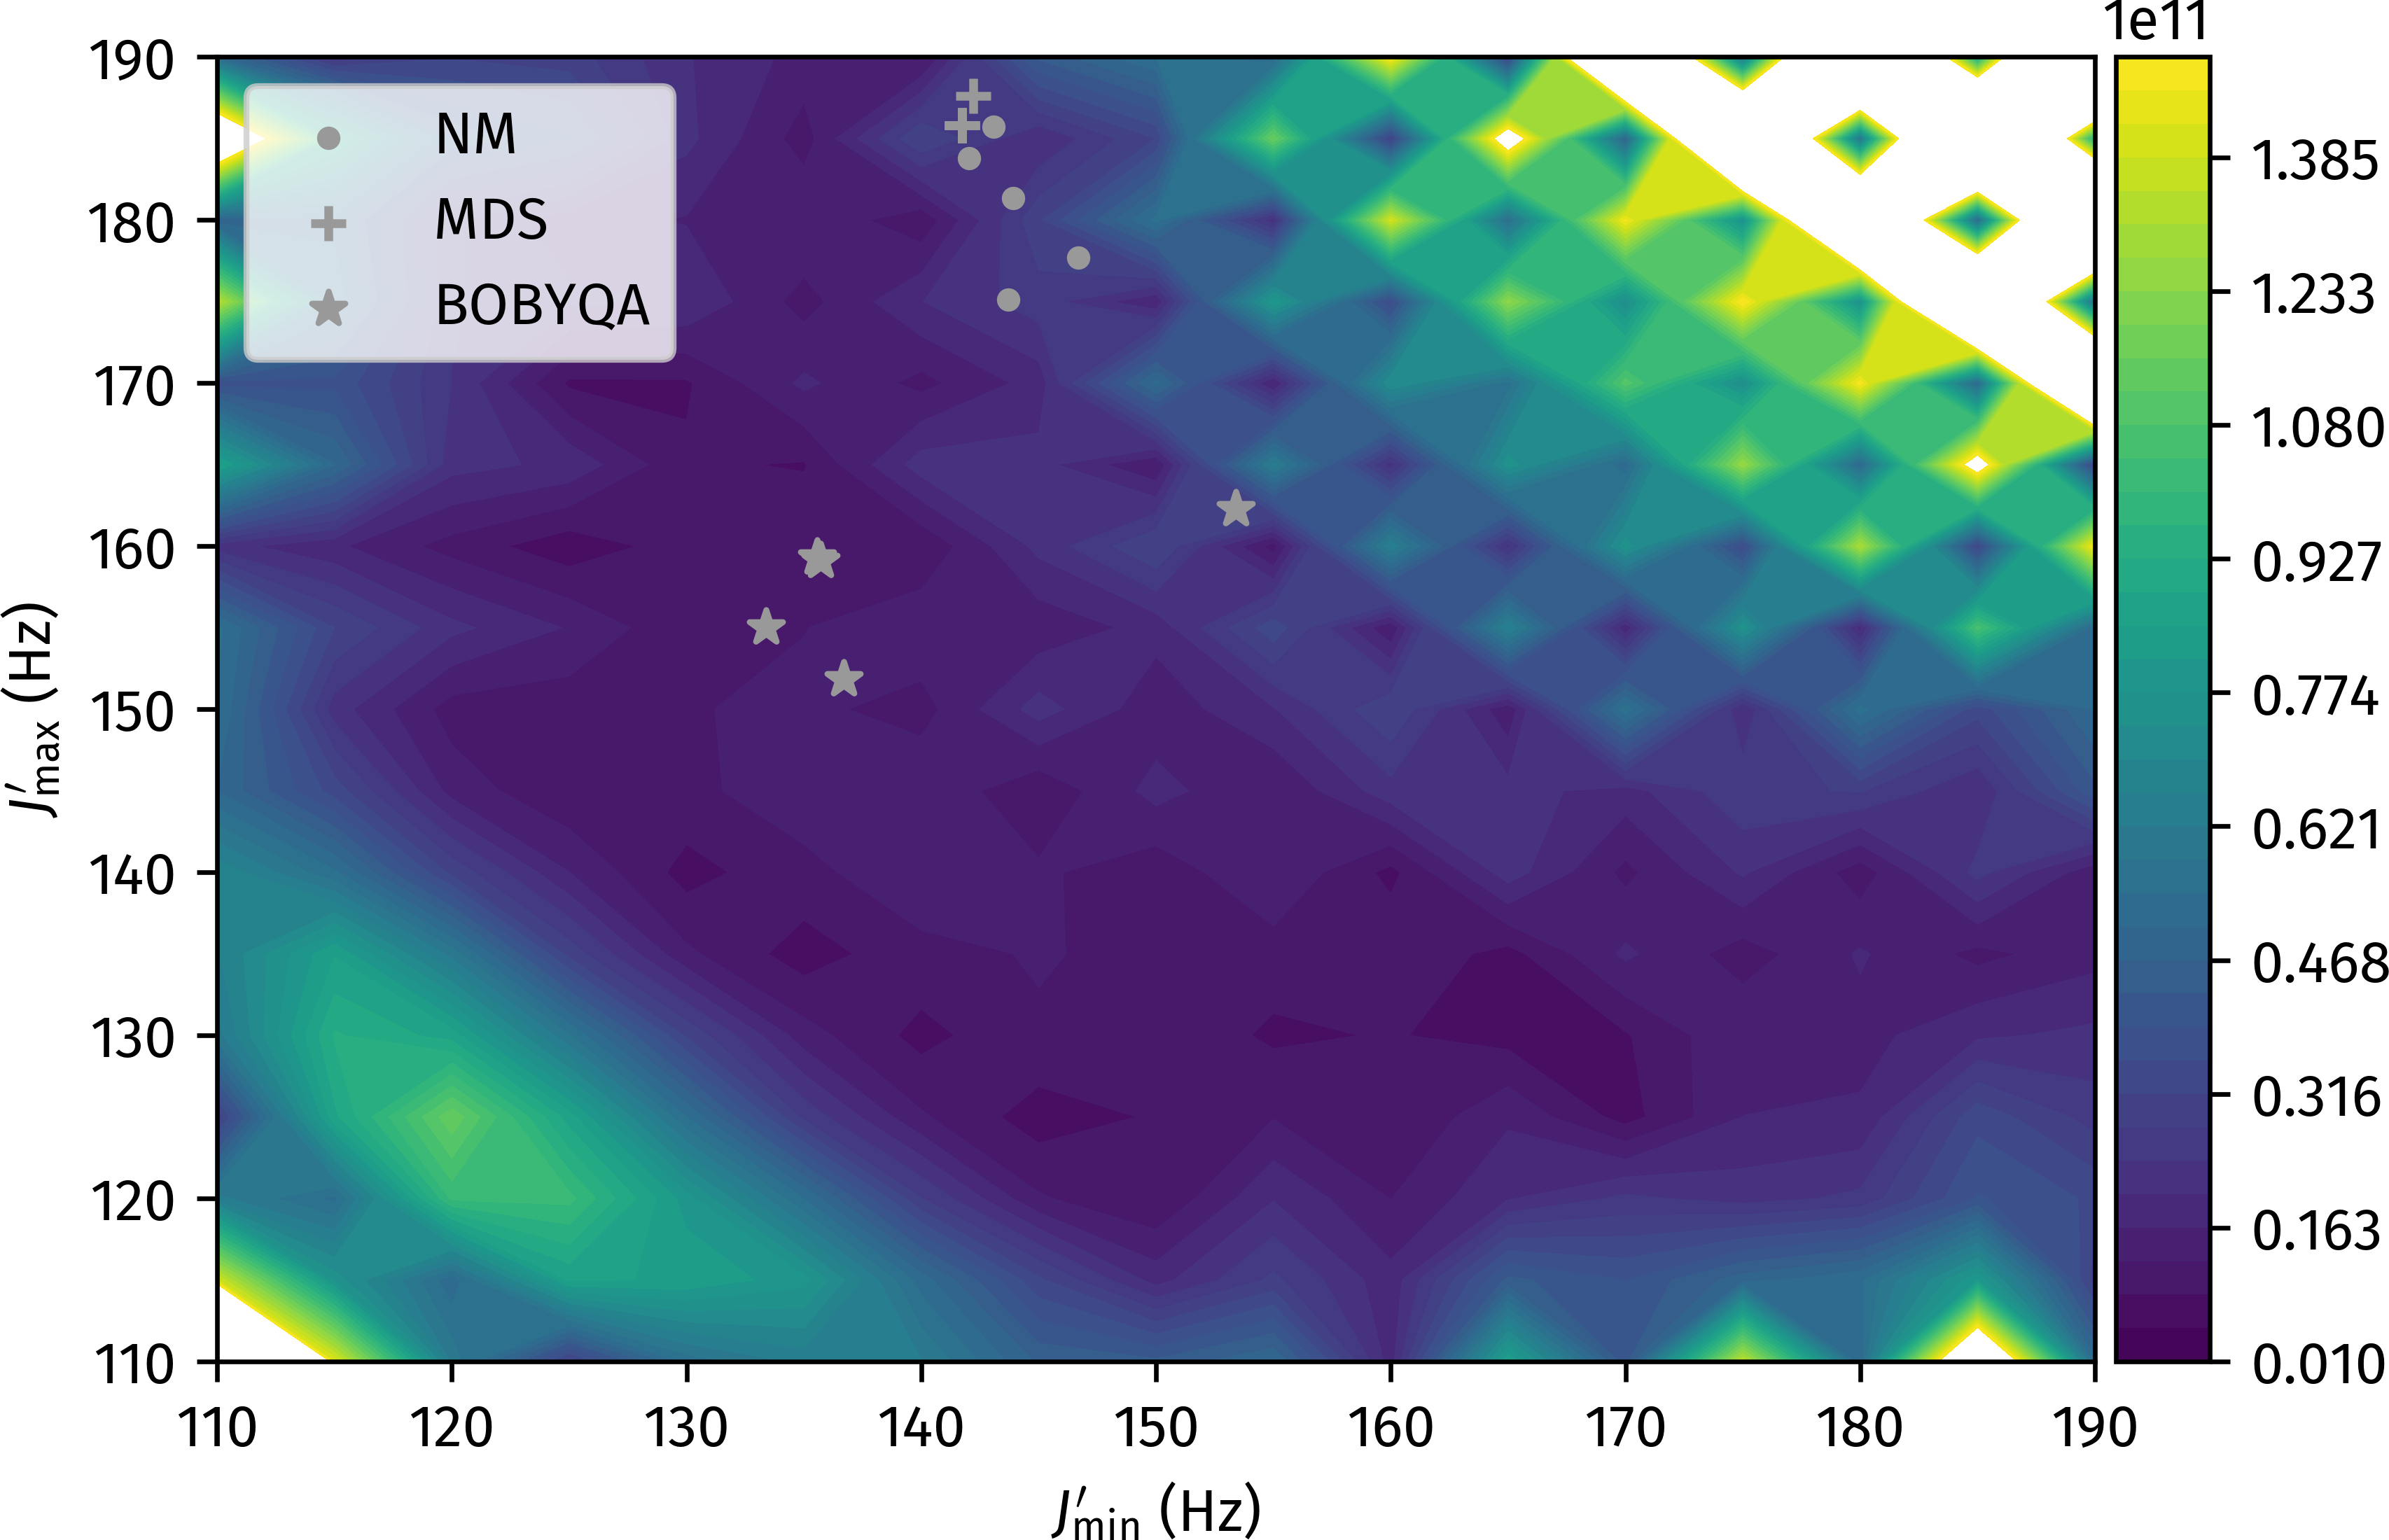
\includegraphics[]{poise/hmbc_scan.png}%
    \caption[Reference grid search for HMBC optimisation]{
        Reference grid search for HMBC optimisation.
        Darker regions correspond to lower cost function values, i.e.\ better spectra.
        The results of the 15 optimisations (5 per algorithm) are plotted on the same axes.
        Note that the cost functions here are rather larger than in \cref{tbl:poise_hmbc}: this is solely because a different receiver gain was used.
        \datacode{7Z-210814}
    }
    \label{fig:poise_hmbc_scan}
\end{figure}

Interestingly, BOBYQA finds an optimum which is different from---and substantially better than---the other two algorithms.
As mentioned previously, it is not generally possible to predict which optimum an algorithm will converge to, and this is complicated even further by the presence of noise, which imparts some stochastic character to the optimisation.
Nevertheless, the other runs actually show that similar optima are reproducibly obtained: the optima found from each of the five rounds, as well as a reference grid search, are plotted in \cref{fig:poise_hmbc_scan}.
It appears that the simplex-based methods get stuck in a suboptimal region, whereas BOBYQA is able to move leftwards and downwards into a more productive region (with one exception).
However, the exact reasons for this remain unclear.

\begin{figure}[htb]
    \centering
    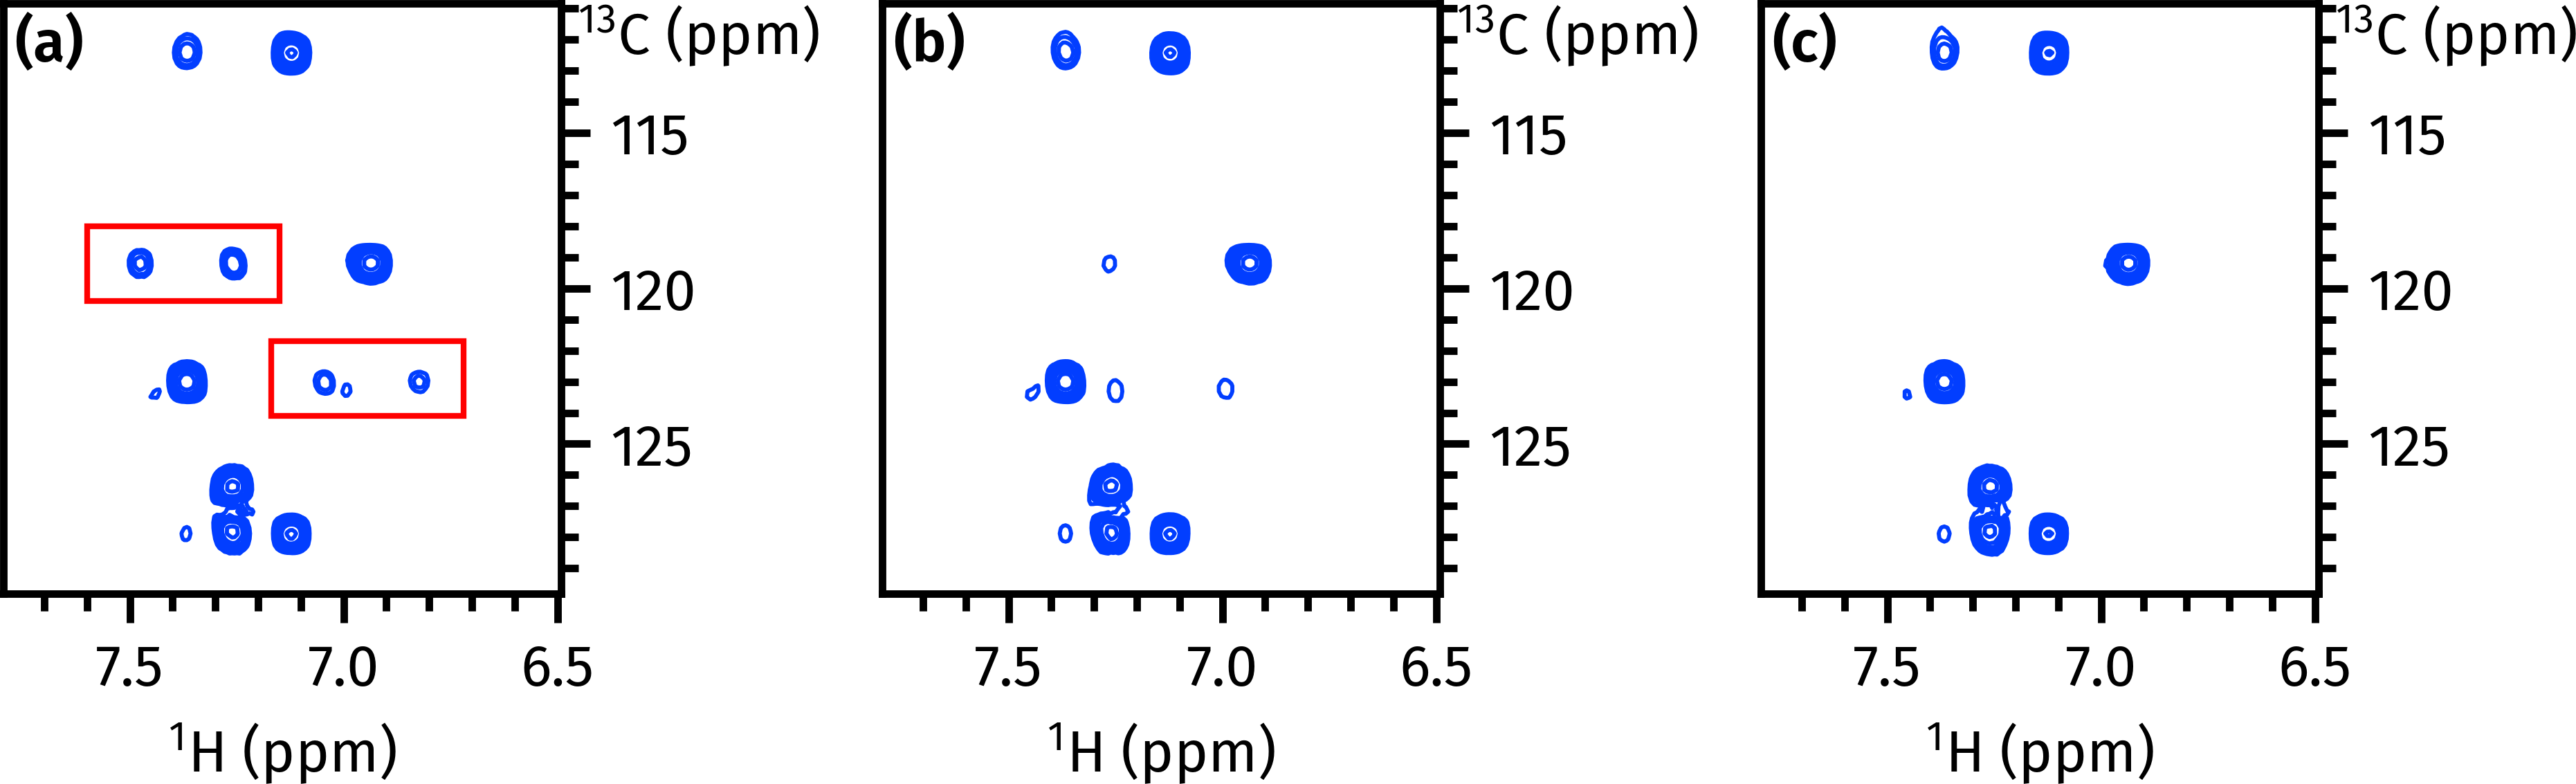
\includegraphics[]{poise/hmbc_spec.png}%
    {\phantomsubcaption\label{fig:poise_hmbc_spec_unopt2}}%
    {\phantomsubcaption\label{fig:poise_hmbc_spec_opt2}}%
    {\phantomsubcaption\label{fig:poise_hmbc_spec_3}}%
    \caption[HMBC spectra before and after optimisation]{
        \textbf{(\subref{fig:poise_hmbc_spec_unopt2})} HMBC spectrum with `compromise' values of 120 and \SI{180}{\Hz} for $J_\text{min}$ and $J_\text{max}$ respectively in the second-order LPJF.
        The one-bond artefacts are highlighted in red boxes.
        \textbf{(\subref{fig:poise_hmbc_spec_opt2})} HMBC spectrum with optimised second-order LPJF delays.
        \textbf{(\subref{fig:poise_hmbc_spec_3})} HMBC spectrum with third-order LPJF.
        \datacode{7Z-210814}
    }
    \label{fig:poise_hmbc_spec}
\end{figure}

In any case, when the best of these optimised values (i.e.\ entry 3 in \cref{tbl:poise_hmbc}) were used to run a standard 2D HMBC, a significant reduction in one-bond artefacts was observed.
The performance of the optimised second-order LPJF was in fact almost comparable to that of a third-order LPJF (\cref{fig:poise_hmbc_spec}).
(However, using a third-order LPJF risks suppressing some of the desired HMBC signal as well, so if all else is equal, the optimised second-order LPJF should be preferred.)


\subsubsection{Application to NOAH HMBC}

\begin{figure}[htb]
    \centering
    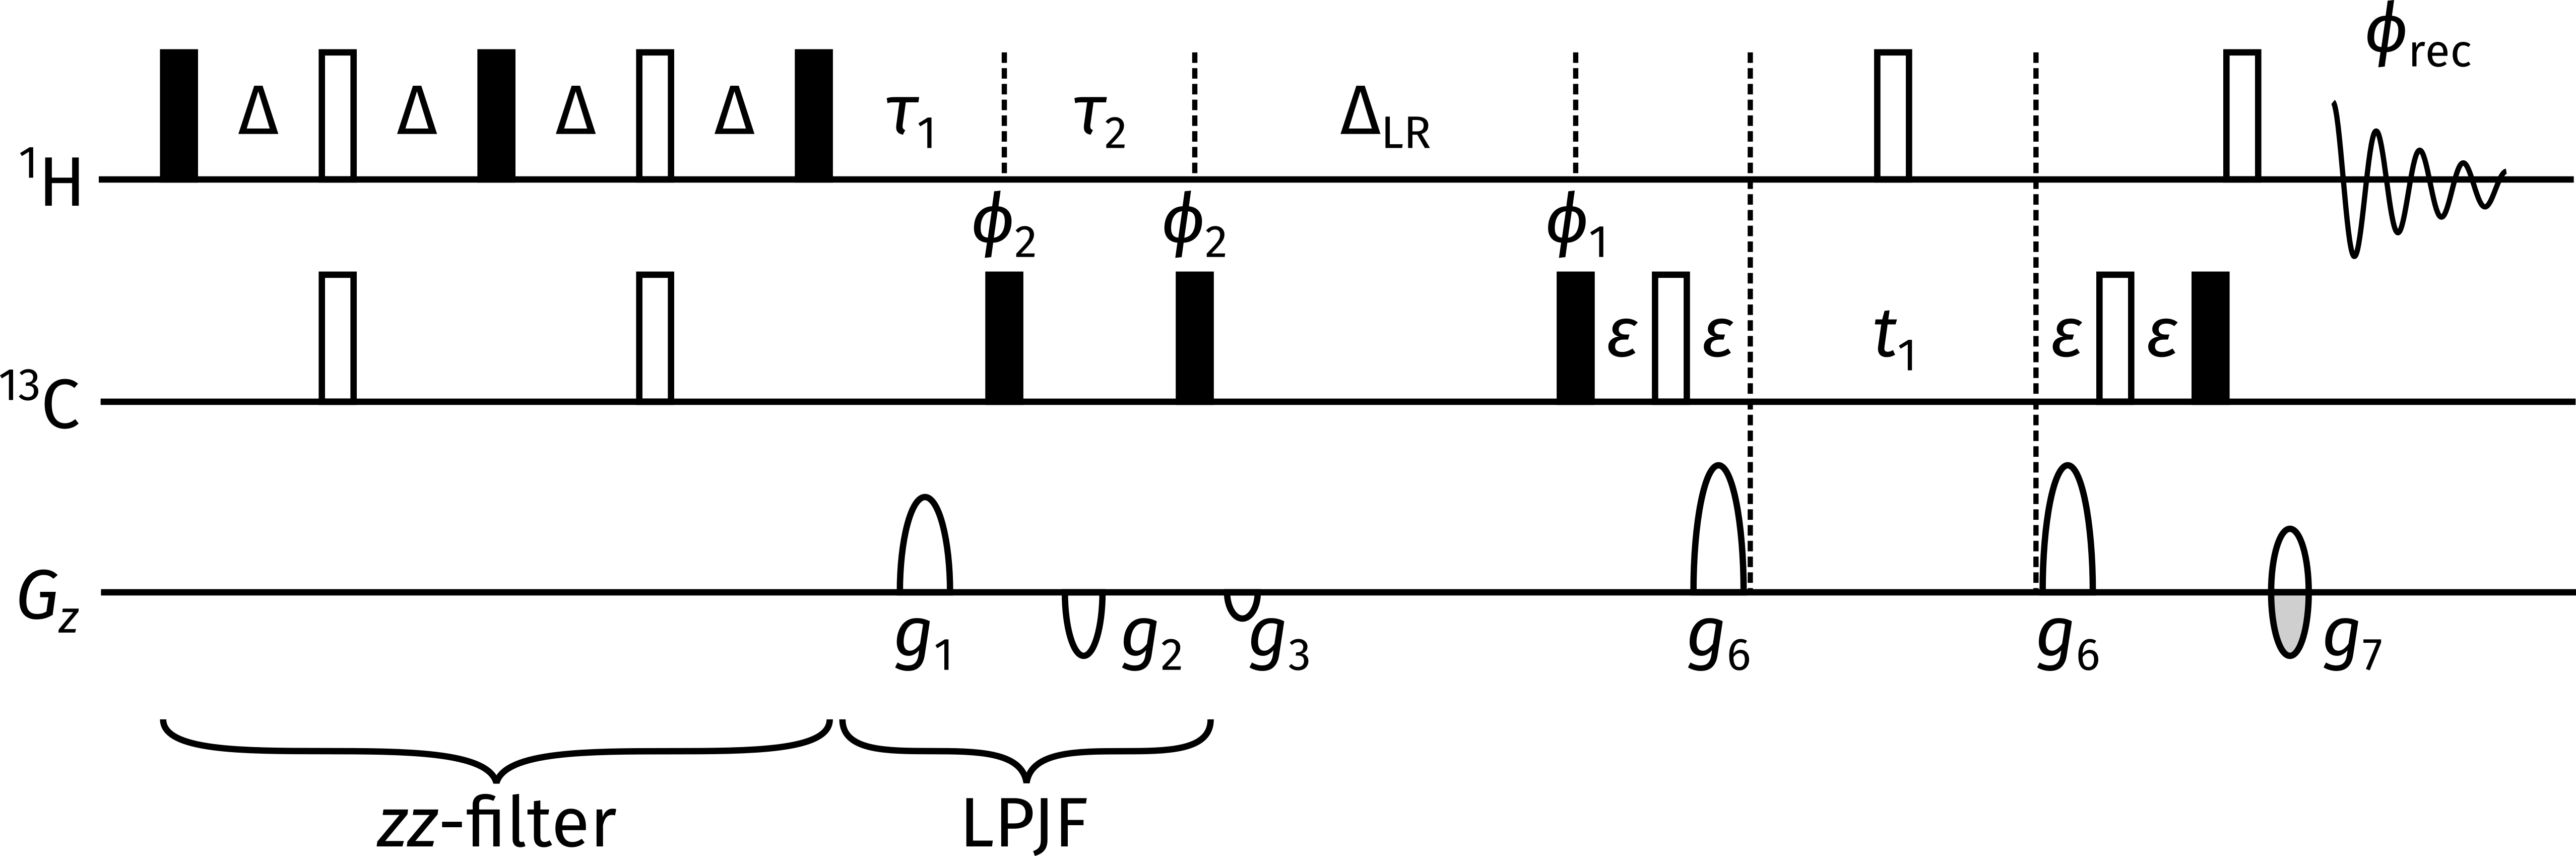
\includegraphics[]{pp/hmbc/noah_no90.png}%
    \caption[NOAH HMBC module used for optimisations]{
        NOAH HMBC module used for POISE optimisations.
    }
    \label{fig:noah_hmbc_no90}
\end{figure}

In NOAH supersequences, the HMBC experiment (or `module') is typically modified by replacing the initial \ang{90} excitation pulse with a $zz$-filter (\cref{fig:noah_hmbc_no90}).
This causes the \magnnot{C} magnetisation used in the HMBC to be excited, but leaves \magn{C} magnetisation along the $+z$ axis so that it can be preserved for later modules in a supersequence.
In an ideal situation, this means that the one-bond artefacts in the HMBC should in fact be suppressed even without an LPJF.
However, significant one-bond artefacts are in fact still observed in NOAH HMBC spectra.
I therefore sought to apply the same optimisation routine to the $zz$-HMBC module to see whether this could be improved.


\begin{table}[htb]
    \hbadness=10000
    \centering
    \begin{tabular}{ccccccc}
        \toprule
              &           & \multicolumn{3}{c}{Best optimum found} & \multicolumn{2}{c}{Aggregated results} \\
        \cmidrule(lr){3-5} \cmidrule(lr){6-7}
        Entry & Algorithm & $J_\text{min}$ & $J_\text{max}$ & $f_\text{sos} / 10^9$ & FEs & Time taken (\si{\s}) \\
        \midrule
        1     & NM        & 117.05 & 188.59                 & 5.37 & 25--29 & 451--523 \\
        2     & MDS       & 125.21 & 193.16                 & 5.35 & 14--17 & 249--310 \\
        3     & BOBYQA    & 119.49 & 182.74                 & 5.78 & 9--16  & 164--293 \\
        \bottomrule
    \end{tabular}
    \caption[NOAH HMBC low-pass J-filter optimisations]{
        Results of POISE optimisations on the LPJF in the NOAH HMBC module.
        All optimisation details are the same as in \cref{tbl:poise_hmbc}, except that the LPJF--HSQC pulse sequence used for the optimisation was modified accordingly to include a $zz$-filter.
        \datacode{7Z-210814}
    }
    \label{tbl:poise_hmbc_noah}
\end{table}

Unfortunately, the results here were far less impactful: generally, the optimisation converged to values very close to the initial starting point, and in some cases the behaviour of the optimised spectrum was even (very slightly) worse than the unoptimised spectrum.
(The deterioration is very marginal, and likely arises only due to noise in the cost function during the optimisation.)
This strongly suggests that the artefacts are not due to imperfect LPJF suppression, but instead stem from the $zz$-filter component of the sequence.
This was indeed verified experimentally: the addition of a \carbon{} \ang{90} pulse at the end of the $zz$-filter led to much better one-bond artefact suppression (\cref{fig:poise_hmbc_noah_spec_with90}; this strategy is further explained in \todo{SECTION}).

\begin{figure}[htb]
    \centering
    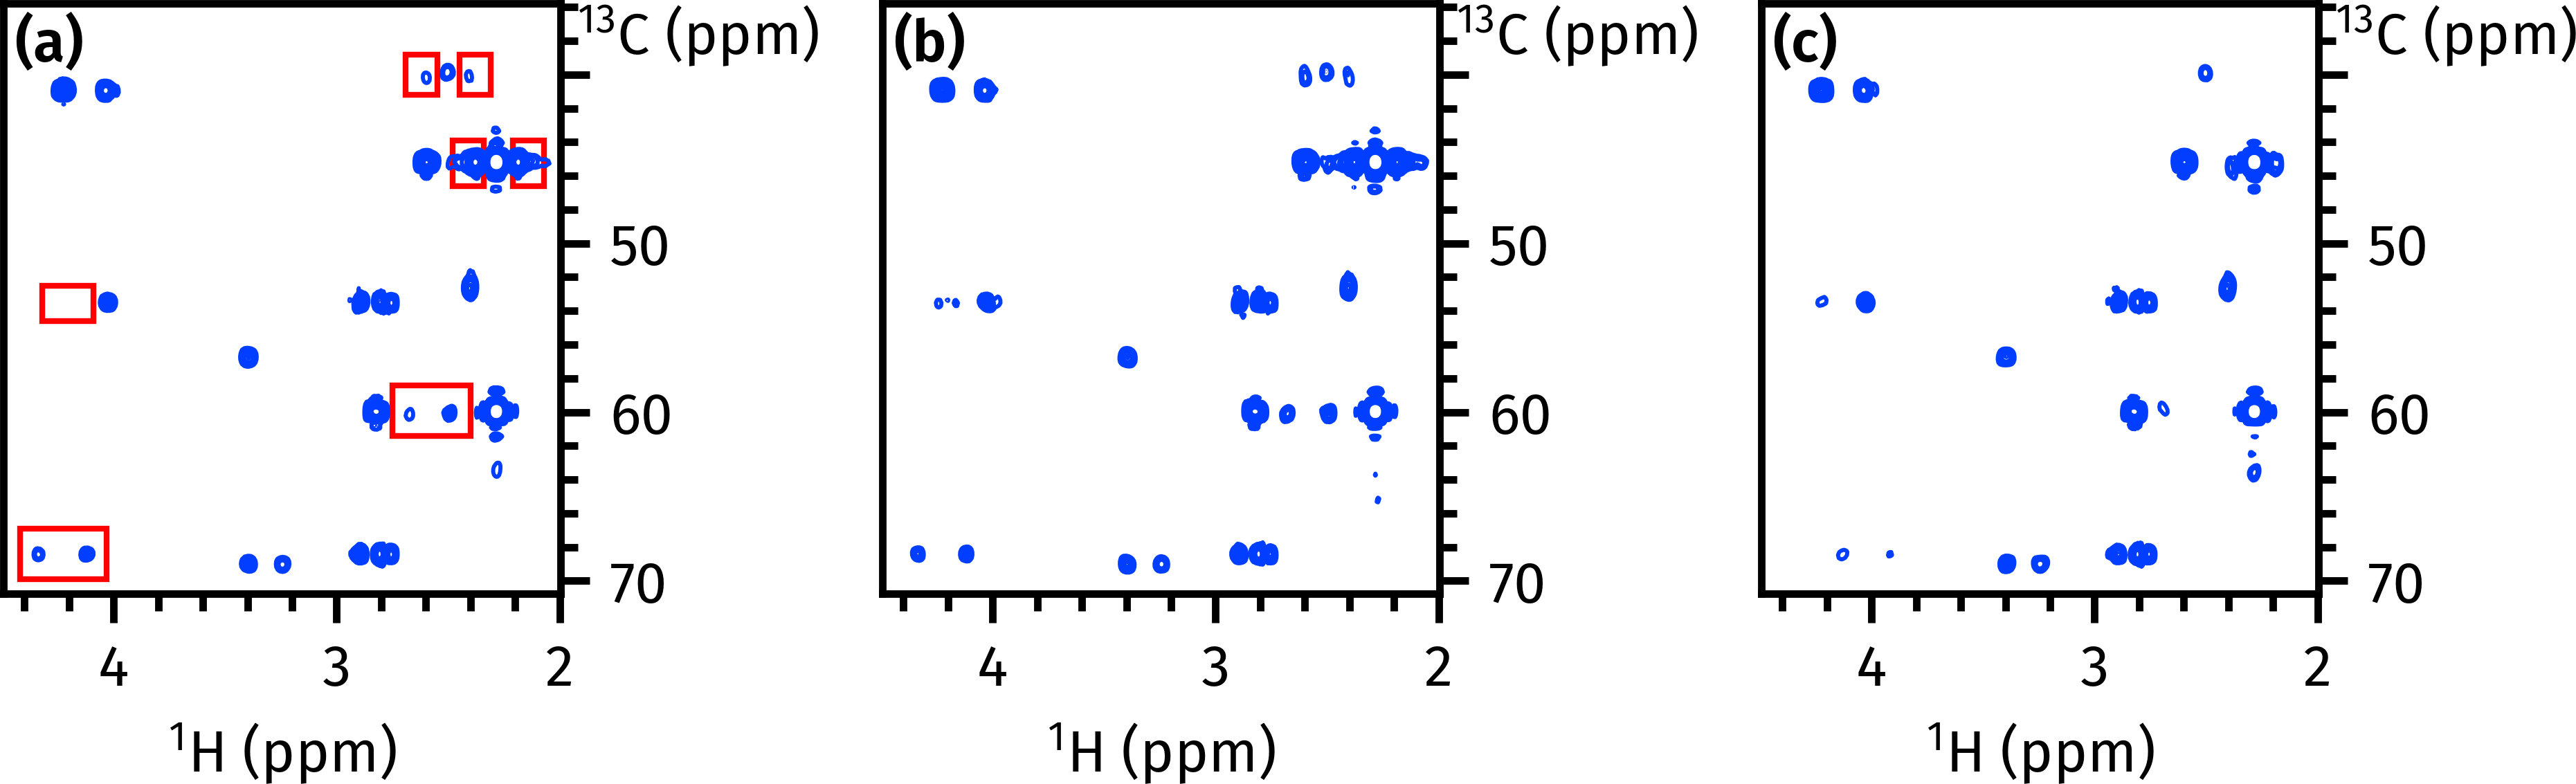
\includegraphics[]{poise/hmbc_noah_spec.png}%
    {\phantomsubcaption\label{fig:poise_hmbc_noah_spec_unopt}}%
    {\phantomsubcaption\label{fig:poise_hmbc_noah_spec_opt}}%
    {\phantomsubcaption\label{fig:poise_hmbc_noah_spec_with90}}%
    \caption[NOAH HMBC spectra before and after optimisation]{
        \textbf{(\subref{fig:poise_hmbc_noah_spec_unopt})} NOAH HMBC spectrum before POISE optimisation, using the default settings of 120 and \SI{180}{\Hz}.
        One-bond artefacts are highlighted in red boxes.
        \textbf{(\subref{fig:poise_hmbc_noah_spec_opt})} NOAH HMBC spectrum after POISE `optimisation' (using $J_\text{min} = \SI{125.2}{\Hz}$, $J_\text{max} = \SI{193.2}{\Hz}$, as per entry 2 of \cref{tbl:poise_hmbc_noah}).
        \textbf{(\subref{fig:poise_hmbc_noah_spec_with90})} NOAH HMBC spectrum with no POISE optimisation, but instead adding a \ang{90} \carbon{} pulse at the end of the $zz$-filter (see also \todo{SECTION}).
        \datacode{7Z-210814}
    }
    \label{fig:poise_hmbc_noah_spec}
\end{figure}

\subsection{PSYCHE pure shift NMR}
\label{subsec:poise__psyche}

In \cref{sec:pureshift__optimisation}, I described the motivation behind, and early attempts towards, the optimisation of PSYCHE pure shift spectra.
The content in this section is similar, except that it was performed within the framework of POISE.

\begin{figure}[htb]
    \centering
    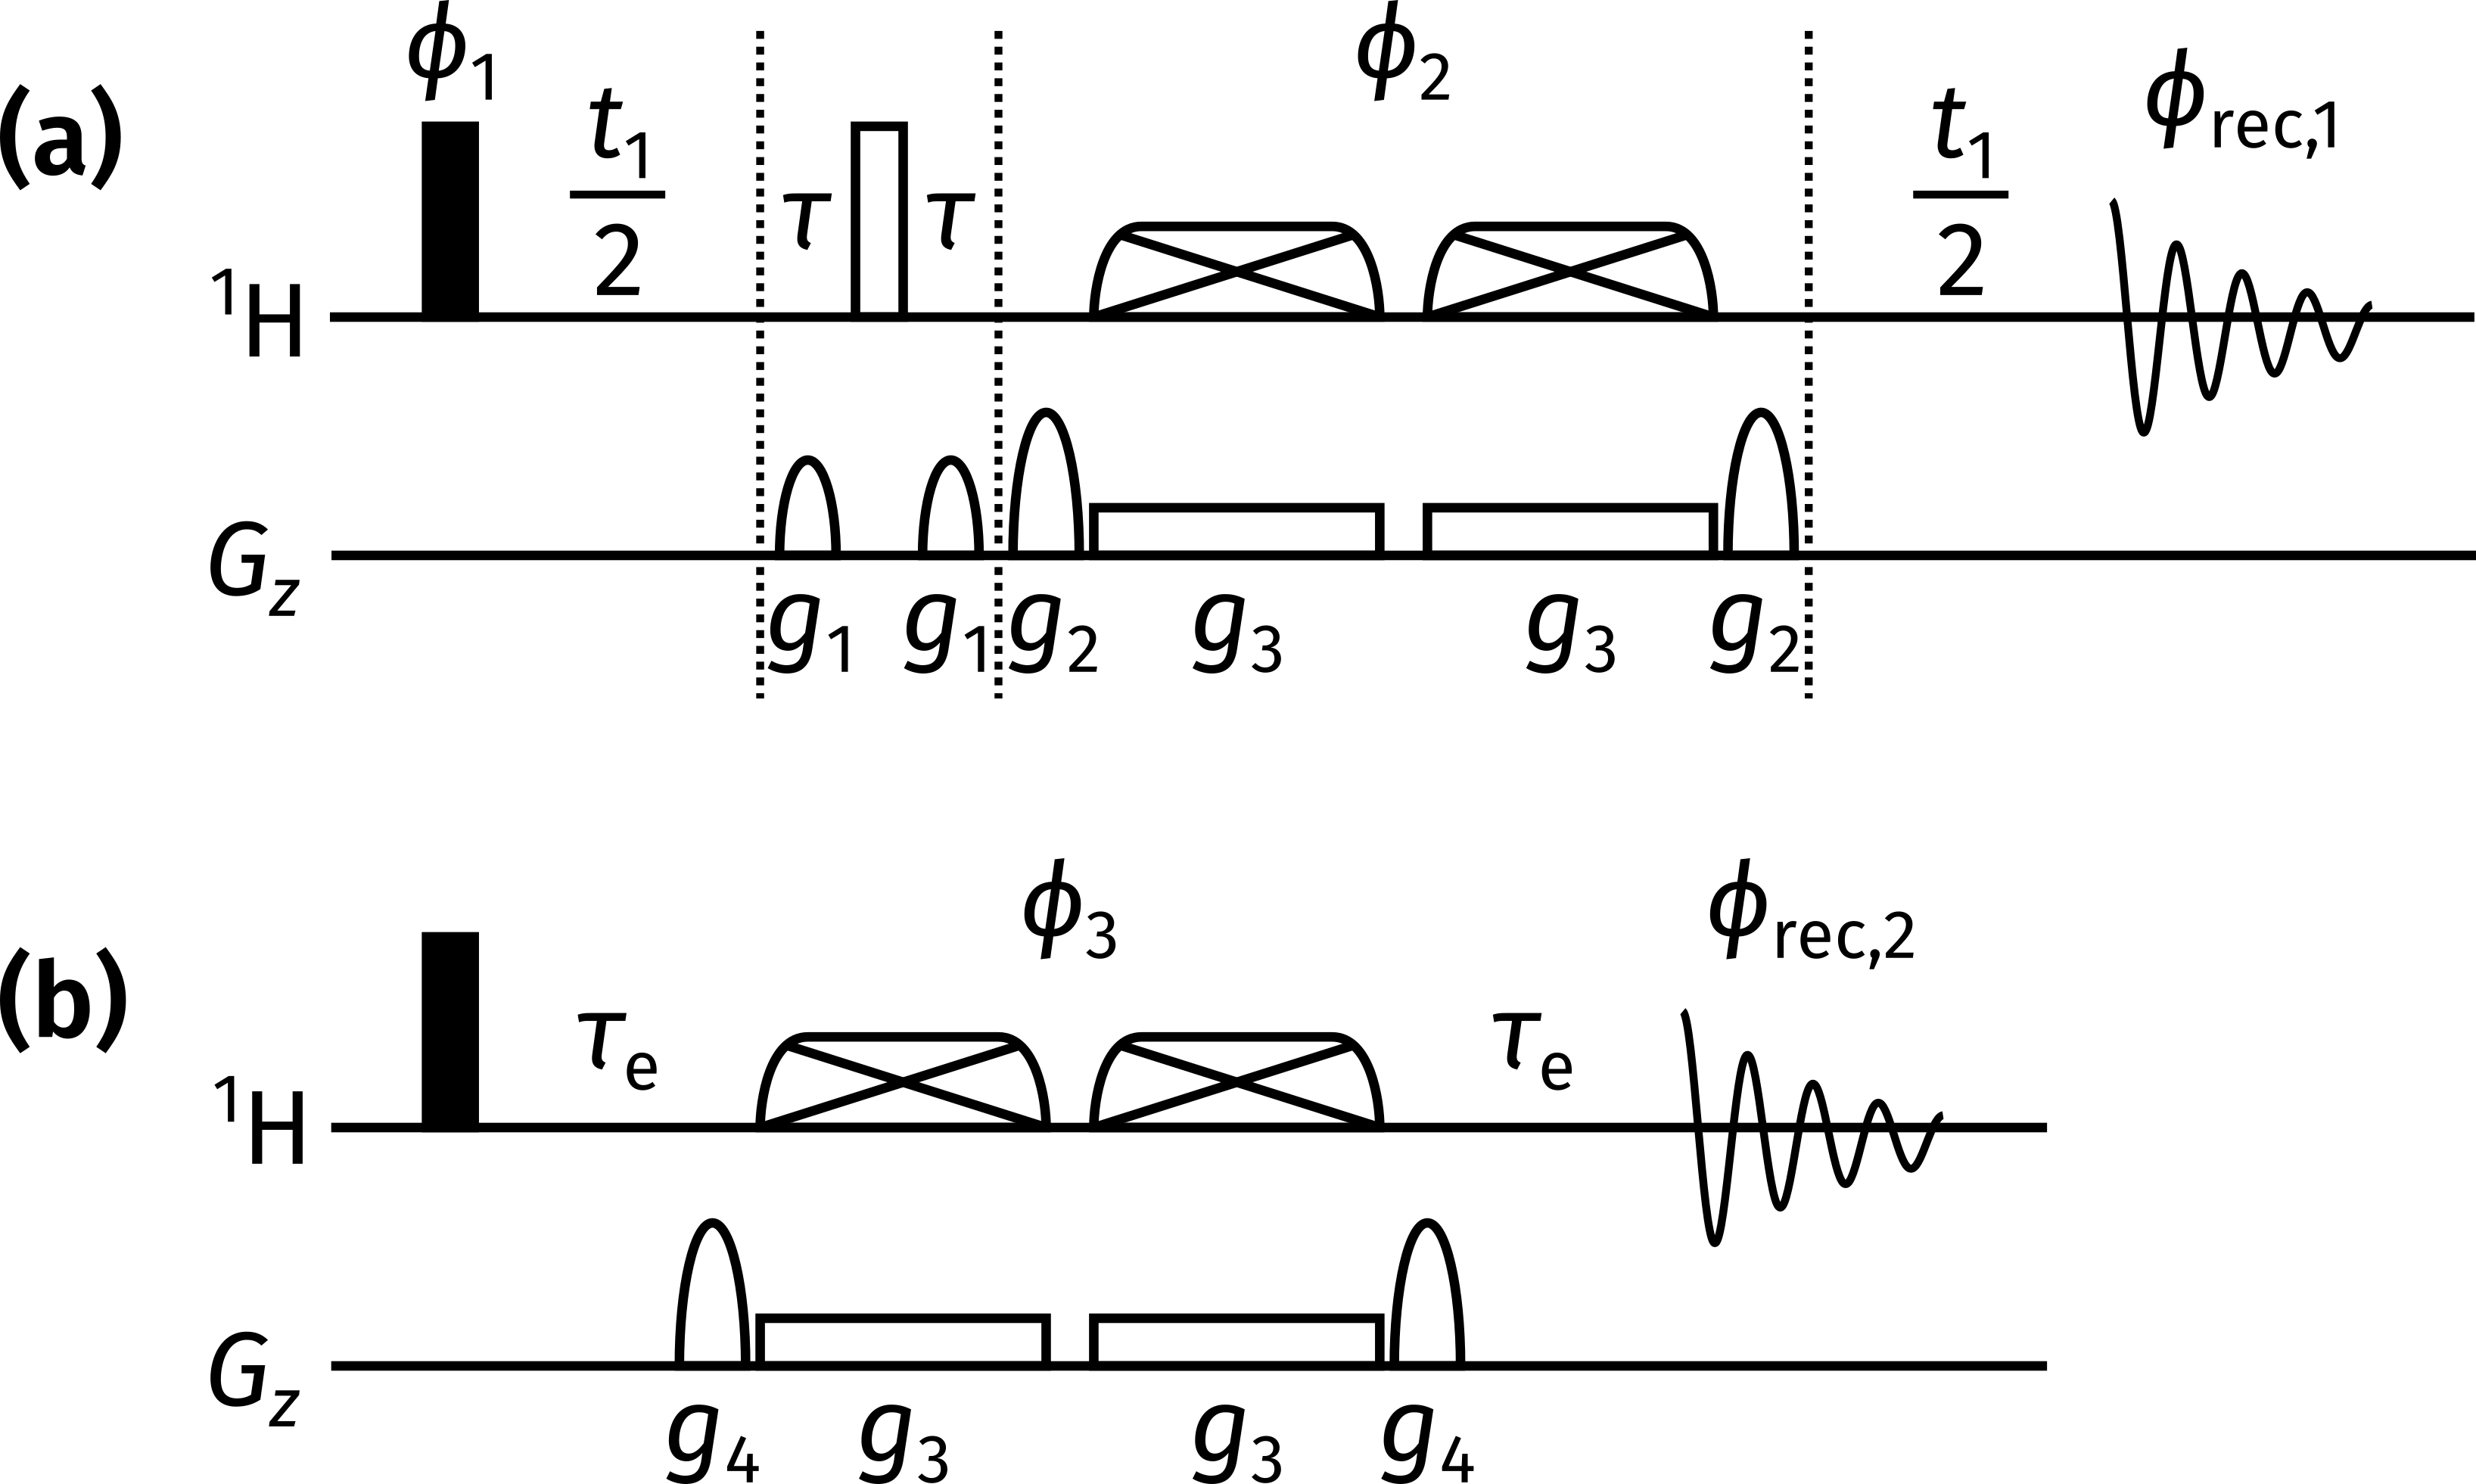
\includegraphics[]{pp/poise/psyche.png}%
    {\phantomsubcaption\label{fig:poise_psyche_pulseq_psyche}}%
    {\phantomsubcaption\label{fig:poise_psyche_pulseq_jrse}}%
    \caption[Pulse sequences used for PSYCHE optimisations]{
        \textbf{(\subref*{fig:poise_psyche_pulseq_psyche})} Pseudo-2D PSYCHE pure shift experiment.
        \textbf{(\subref*{fig:poise_psyche_pulseq_jrse})} J-resolved spin echo experiment (see also \cref{subsec:pureshift__optim_techniques}) using the PSYCHE PSE.
        Phase cycling is performed using: $\phi_1 = (x, -x)$, $\phi_2 = (x, x, y, y)$, $\phi_{\text{rec},1} = (x, -x, -x, x)$ for the full PSYCHE experiment, and $\phi_3 = (x, y, -x, -y)$, $\phi_{\text{rec},2} = (x, -x, x, -x)$ for the JRSE experiment.
        CTP gradient amplitudes are $(g_1, g_2, g_4) = (35\%, 77\%, 50\%)$ (though the exact values are likely immaterial); the PSYCHE gradient $g_3$ was subjected to optimisation.
        The delay $\tau$ is set to $1/(4 \cdot T_\text{chunk})$ for the PSYCHE experiment, and $\tau_\text{e}$ is \qty{16}{\ms}.
    }
    \label{fig:poise_psyche_pulseq}
\end{figure}



\subsubsection{Optimisation setup}

In this section, the standard double-saltire PSYCHE pure shift element was used (\cref{fig:poise_psyche_pulseq_psyche}).\autocite{Foroozandeh2014ACIE,Foroozandeh2018CEJ}
As described in \cref{subsec:pureshift__optim_techniques}, the PSYCHE PSE can be described using six parameters; in this section, we investigate only three of these, namely the amplitude (i.e.\ flip angle $\beta$), bandwidth $\Delta F$, and duration $\taup$.
In addition to this, the amplitude of the weak gradient during the PSE $g_3$ was also chosen as a fourth parameter to vary.
As before, the quality of the PSE is evaluated using a JRSE experiment (\cref{fig:poise_psyche_pulseq_jrse}), which is then compared against a pulse--acquire spectrum: the cost function used is $f_\text{diff}$.

In the JRSE pulse sequence used for optimisation, the four parameters (flip angle, bandwidth, duration, and gradient amplitude) are respectively \texttt{CNST20}, \texttt{CNST21}, \texttt{P40}, and \texttt{GPZ10}.
There is, however, a slight complication: whenever the bandwidth or duration is changed, the entire pulse must be re-created, because the $x$- and $y$-coefficients depend on these parameters.
Therefore, a (TopSpin) Python script was written to generate the double saltire pulse using the parameters above, and the POISE AU programme was modified to call this Python script before acquiring the spectrum.
Although the overall setup may perhaps be slightly confusing,%
\footnote{We have here a Python script (the POISE frontend) calling an AU programme (for acquisition) which calls a Python script (to make the double saltire).}
I contend that this is an excellent demonstration of the customisability that POISE provides.

One slightly odd behaviour noted with the PSYCHE optimisations was that at least one dummy scan was required for the optimisation to be robust:
if no dummy scans were used, the \textit{very first} FE in an optimisation run would yield a rather unreliable result, although subsequent FEs were unaffected.
It is not obvious why this is the case, as FEs are already separated by a delay of several seconds, which is on the order of $5T_1$: thus, each FE should be starting from (almost) full equilibrium magnetisation.
Nevertheless, to avoid this issue, all optimisations in this section were run using \texttt{DS=1} and \texttt{NS=2}.

The sample used was andrographolide: this is the same sample as was used in the dPSYCHE section (\cref{sec:pureshift__dpsyche}), and is fairly useful for pure shift studies as it contains quite diverse coupling patterns.
The spectral region was limited to \qty{1.15}{\ppm} and above to exclude strong singlets from the methyl groups in andrographolide, which are irrelevant to pure shift NMR but disproportionately influence the value of the cost function (this issue was also discussed in \cref{subsec:pureshift__chirpopt}).


\subsubsection{Optimisation results}

\begin{table}
    \centering
    \begin{tabular}{cccccccc}
        \toprule
         & \multicolumn{3}{c}{Aggregated results from all runs} & \multicolumn{4}{c}{Parameters from best optimum} \\
        \cmidrule(lr){2-4} \cmidrule(lr){5-8}
        Description & $f_\mathrm{diff}$ & FEs              & Time (\unit{\s}) & $\beta$ ($^\circ$) & $g_3$ (\%) & $\Delta F$ (kHz) & $\tau_\mathrm{p}$ (ms) \\
        \midrule
        Initial point & 0.353        & --     & --        & (25.0) & (2.00) & (10.0) & (30.0) \\
        1 parameter   & 0.340--0.343 & 5--10  & 84--168   & 17.5   & (2.00) & (10.0) & (30.0) \\
        2 parameters  & 0.325--0.338 & 12--33 & 205--565  & 16.5   & 1.00   & (10.0) & (30.0) \\
        3 parameters  & 0.320--0.328 & 18--77 & 315--1344 & 17.4   & 1.73   & 15.9   & (30.0) \\
        4 parameters  & 0.316--0.333 & 39--85 & 705--1504 & 13.9   & 1.45   & 15.9   & 36.0   \\
        \bottomrule
    \end{tabular}
    \caption[Overview of all PSYCHE optimisations]{
        Summary of all optimisations performed on the PSYCHE PSE.
        Unlike before, aggregated results are not grouped by optimisation algorithm; these ranges are therefore collected from a total of 15 runs (5 per algorithm).
        Parameters in parentheses were not optimised and were simply carried over from the initial point.
        A detailed breakdown of the results by algorithm, as well as the POISE routines used, are described in \cref{tbl:poise_psyche1p,tbl:poise_psyche2p,tbl:poise_psyche3p,tbl:poise_psyche4p}.
        \datacode{6A-200822}
    }
    \label{tbl:poise_psyche_summary}
\end{table}

\begin{figure}[htb]
    \centering
    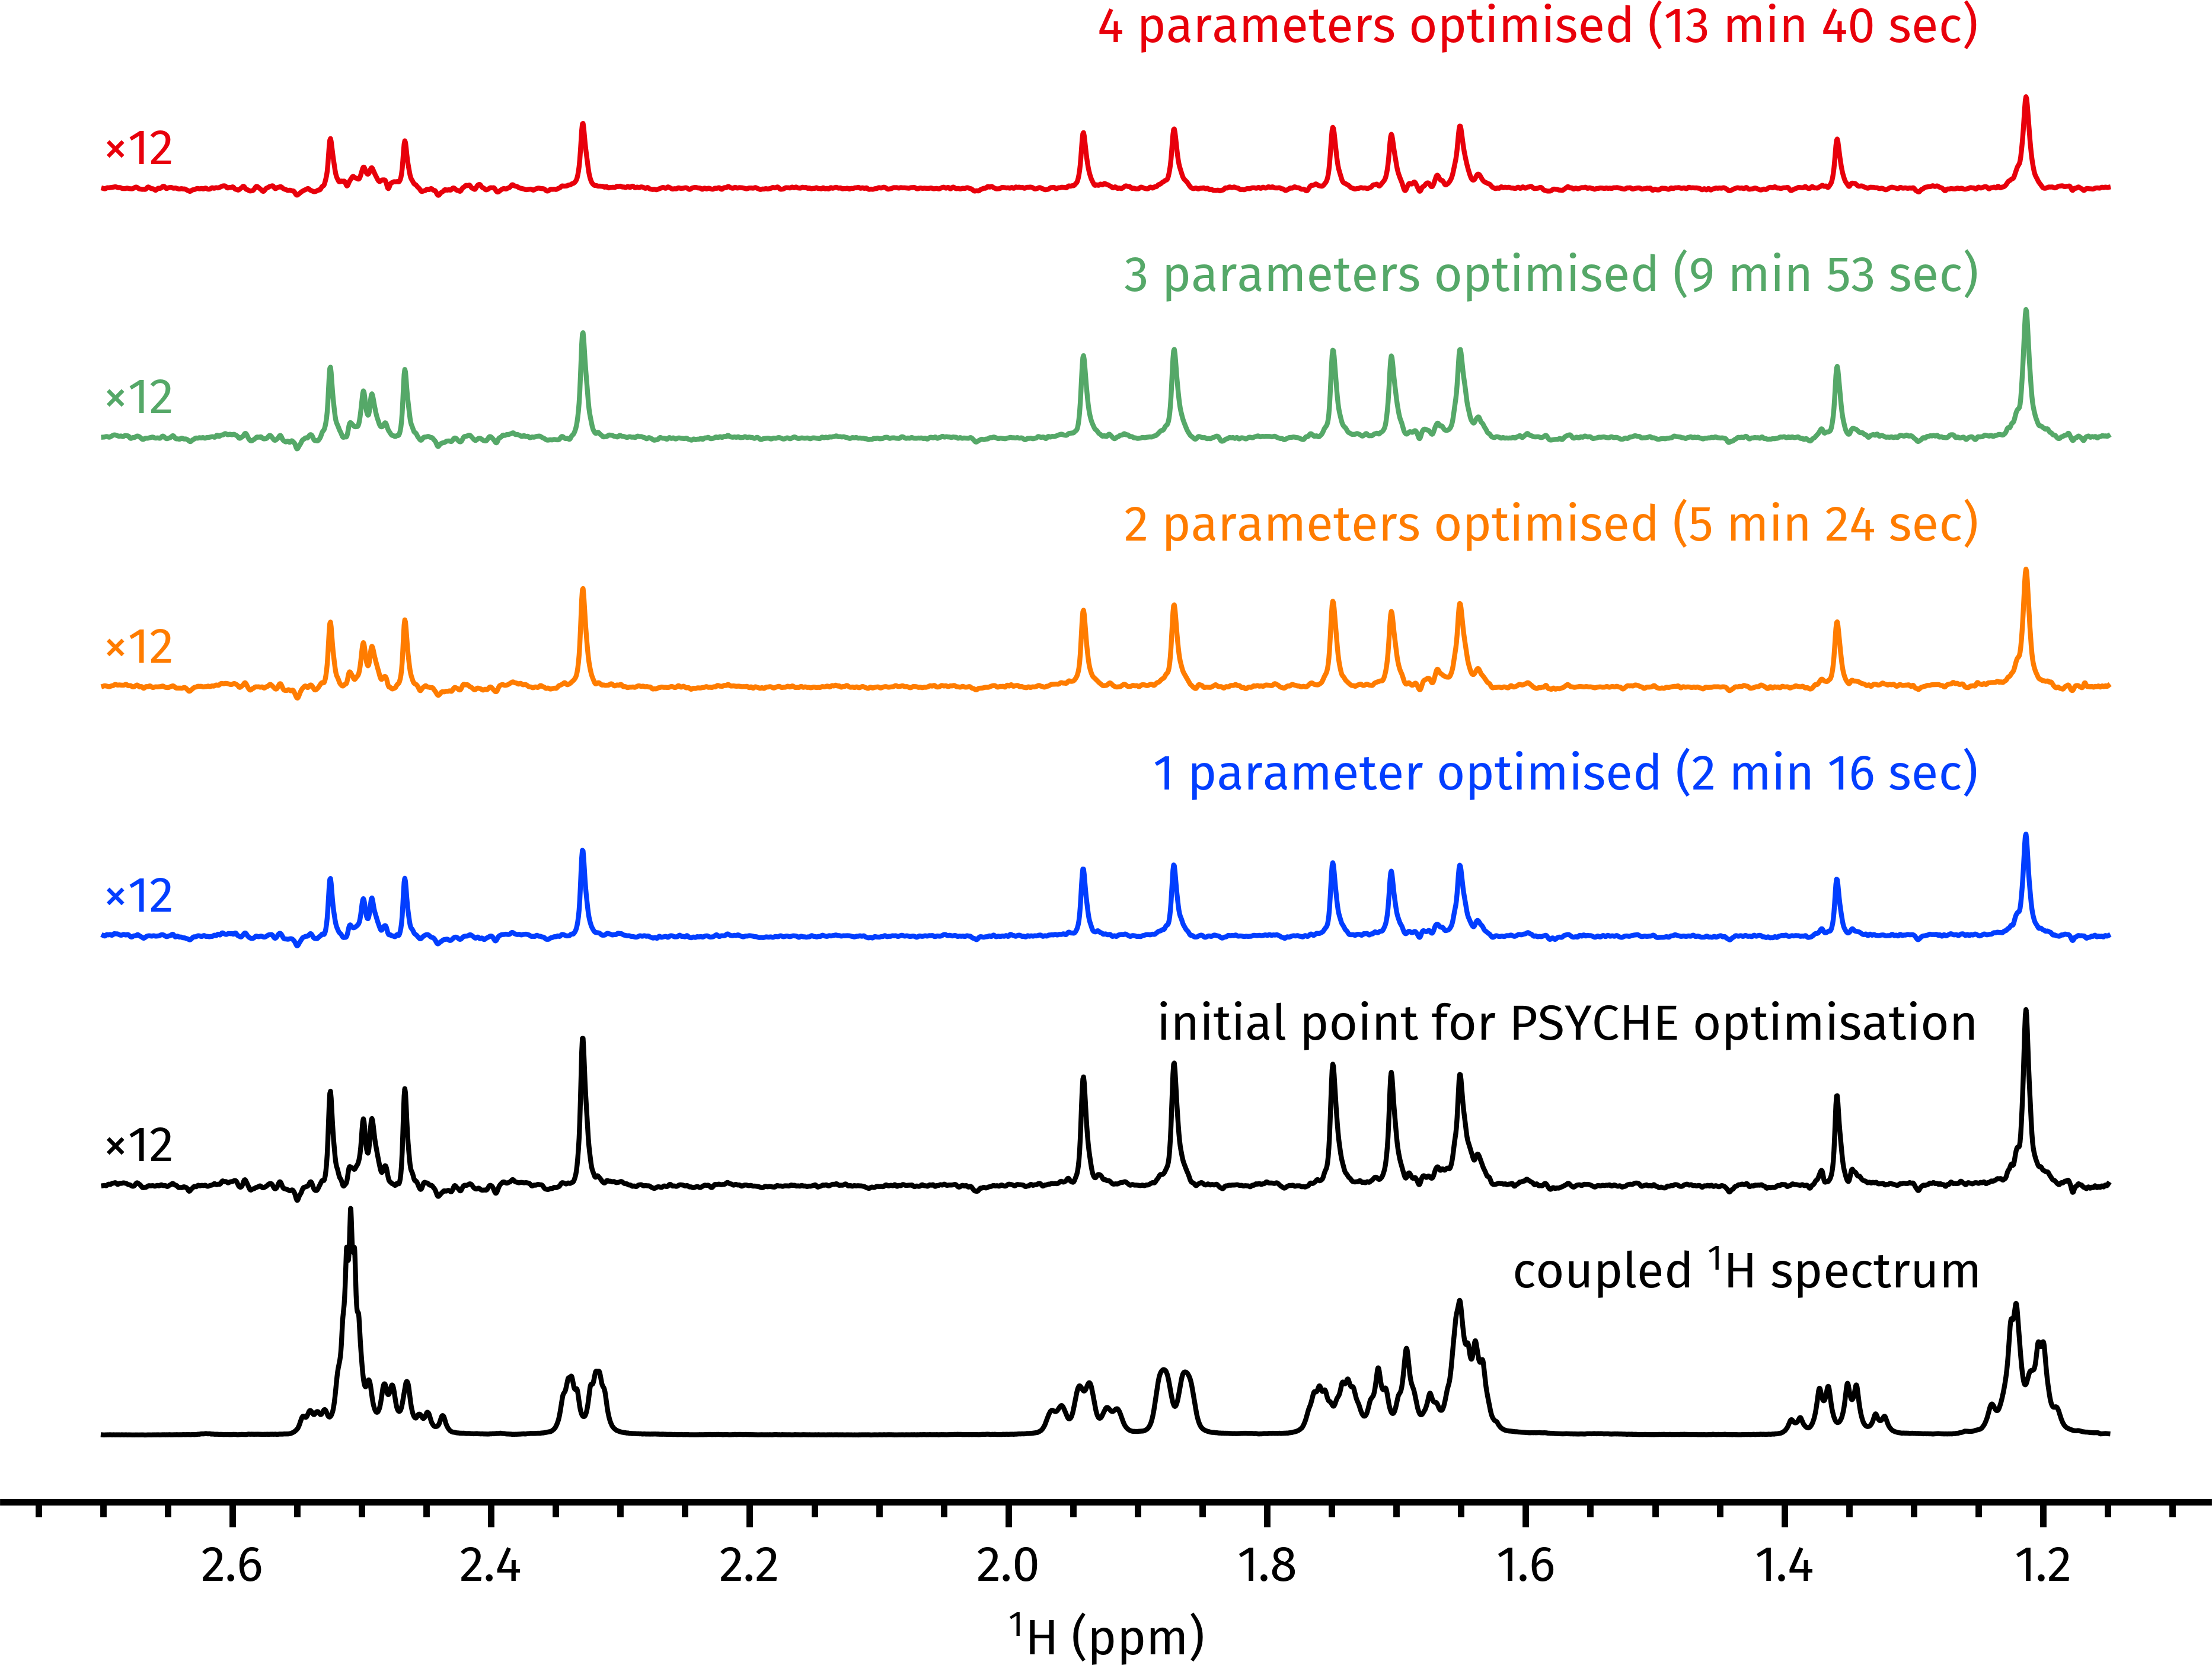
\includegraphics[]{poise/psyche_spec.png}%
    \caption[PSYCHE spectra before and after optimisation]{
        Insets of PSYCHE spectra obtained using the best optimum from each set of optimisations in \cref{tbl:poise_psyche_summary}; the time required to obtain the optimised parameters is also indicated for each spectrum.
        The original coupled \proton{} spectrum is shown as a reference.
        \datacode{6A-200823}
    }
    \label{fig:poise_psyche_spec}
\end{figure}

\begin{table}
    \hbadness=10000
    \centering
    \begin{tabular}{ccccc}
        \toprule
       Entry & Algorithm & Optimum found (\unit{\degree}) & FEs   & Time (\unit{\s}) \\
        \midrule
        1     & NM        & 15.0--20.0                   & 8--10 & 135--168             \\
        2     & MDS       & 17.5--20.0                   & 8     & 133--136             \\
        3     & BOBYQA    & 18.4--19.9                   & 5     & 84--85               \\
        \bottomrule
    \end{tabular}
    \caption[PSYCHE one-parameter optimisations]{
        PSYCHE one-parameter (flip angle) optimisations.
        The POISE routine used was: \mintinline[breaklines]{json}{{"name": "psyche1", "pars": ["cnst20"], "lb": [10.0], "ub": [35.0], "init": [25.0], "tol": [2.0], "cf": "specdiff", "au": "poise_1d"}}.
        \datacode{6A-200822}
    }
    \label{tbl:poise_psyche1p}
\end{table}

\begin{table}
    \hbadness=10000
    \centering
    \begin{tabular}{ccccccc}
        \toprule
              &           & \multicolumn{3}{c}{Best optimum found}            & \multicolumn{2}{c}{Aggregated results} \\
                            \cmidrule(lr){3-5}                                  \cmidrule(lr){6-7}
        Entry & Algorithm & $\beta$ ($^\circ$) & $g_3$ (\%) & $f_\text{diff}$ & FEs    & Time (\unit{\s}) \\
        \midrule
        1     & NM        & 16.48              & 1.00       & 0.3253          & 18--24 & 307--410             \\
        2     & MDS       & 18.47              & 0.82       & 0.3261          & 25--33 & 424--565             \\
        3     & BOBYQA    & 15.77              & 0.96       & 0.3279          & 12--16 & 205--271             \\
        \bottomrule
    \end{tabular}
    \caption[PSYCHE two-parameter optimisations]{
        PSYCHE two-parameter (flip angle and gradient amplitude) optimisations.
        The POISE routine used was: \mintinline[breaklines]{json}{{"name": "psyche2", "pars": ["cnst20", "gpz10"], "lb": [10.0, 0.2], "ub": [35.0, 5.0], "init": [25.0, 2.0], "tol": [2.0, 0.2], "cf": "specdiff", "au": "poise_1d"}}.
        \datacode{6A-200822}
    }
    \label{tbl:poise_psyche2p}
\end{table}

\begin{table}
    \hbadness=10000
    \centering
    \begin{tabular}{cccccccc}
        \toprule
              &           & \multicolumn{4}{c}{Best optimum found} & \multicolumn{2}{c}{Aggregated results} \\
                            \cmidrule(lr){3-6}                     \cmidrule(lr){7-8}
        Entry & Algorithm & $\beta$ ($^\circ$) & $g_3$ (\%) & $\Delta F$ (\unit{\kHz}) & $f_\text{diff}$ & FEs    & Time (\unit{\s}) \\
        \midrule
        1     & NM        & 17.40              & 1.73       & 15.93                  & 0.3196          & 33--43 & 576--770             \\
        2     & MDS       & 16.75              & 1.71       & 16.33                  & 0.3215          & 46--77 & 804--1344            \\
        3     & BOBYQA    & 16.48              & 1.65       & 16.71                  & 0.3200          & 18--31 & 315--540             \\
        \bottomrule
    \end{tabular}
    \caption[PSYCHE three-parameter optimisations]{
        PSYCHE three-parameter (flip angle, gradient amplitude, and bandwidth) optimisations.
        The POISE routine used was: \mintinline[breaklines]{json}{{"name": "psyche3", "pars": ["cnst20", "gpz10", "cnst21"], "lb": [10.0, 0.2, 1000.0], "ub": [35.0, 5.0, 20000.0], "init": [25.0, 2.0, 10000.0], "tol": [2.0, 0.2, 500.0], "cf": "specdiff", "au": "poise_psyche"}}.
        \datacode{6A-200822}
    }
    \label{tbl:poise_psyche3p}
\end{table}

\begin{table}
    \hbadness=10000
    \centering
    \begin{tabular}{ccccccccc}
        \toprule
              &           & \multicolumn{5}{c}{Best optimum found} & \multicolumn{2}{c}{Aggregated results} \\
                            \cmidrule(lr){3-7}                       \cmidrule(lr){8-9}
        Entry & Algorithm & $\beta$ ($^\circ$) & $g_3$ (\%) & $\Delta F$ (\unit{\kHz}) & $\taup$ (\unit{\ms}) & $f_\text{diff}$ & FEs    & Time (\unit{\s}) \\
        \midrule
        1     & NM        & 13.87              & 1.45       & 15.93                  & 36.00              & 0.3163          & 40--47 & 733--845       \\
        2     & MDS       & 19.15              & 1.06       & 11.19                  & 36.52              & 0.3185          & 57--85 & 1006--1504     \\
        3     & BOBYQA    & 17.59              & 1.20       & 12.76                  & 43.06              & 0.3178          & 39--62 & 705--1130      \\
        \bottomrule
    \end{tabular}
    \caption[PSYCHE four-parameter optimisations]{
        PSYCHE four-parameter (flip angle, gradient amplitude, bandwidth, and pulse duration) optimisations.
        The POISE routine used was: \mintinline[breaklines]{json}{{"name": "psyche4", "pars": ["cnst20", "gpz10", "cnst21", "p40"], "lb": [10.0, 0.2, 1000.0, 5000.0], "ub": [35.0, 5.0, 20000.0, 75000.0], "init": [25.0, 2.0, 10000.0, 30000.0], "tol": [2.0, 0.2, 500.0, 2000.0], "cf": "specdiff", "au": "poise_psyche"}}.
        \datacode{6A-200822}
    }
    \label{tbl:poise_psyche4p}
\end{table}

I ran several different optimisations of increasing complexity:
\begin{itemize}
    \item one-parameter: flip angle only
    \item two-parameter: flip angle and gradient amplitude
    \item three-parameter: flip angle, gradient amplitude, and bandwidth
    \item four-parameter: flip angle, gradient amplitude, bandwidth, and duration
\end{itemize}

\Cref{tbl:poise_psyche_summary} summarises the results obtained from all optimisations, whereas \cref{tbl:poise_psyche1p,tbl:poise_psyche2p,tbl:poise_psyche3p,tbl:poise_psyche4p} shows more detailed results for each individual set of optimisations, including a breakdown by algorithm.
We can see from these results that---perhaps unsurprisingly---optimising more parameters leads to greater improvements in the cost function, albeit at the cost of more FEs and more time.

An important question is whether these reductions in the cost function (measured on a JRSE experiment) do actually translate into improved pure shift spectra.
The pure shift spectra, obtained with the optimised parameters in \cref{tbl:poise_psyche_summary}, are shown in \cref{fig:poise_psyche_spec}.
Of particular interest are the two strongly coupled protons at \qty{2.5}{\ppm}: in the pure shift spectrum, the two peaks on either side are genuine, but strong coupling artefacts appear in the middle of these peaks.
On top of that, the decoupling performance for the peaks at \qty{1.36}{\ppm} and \qty{1.65}{\ppm} are also worth noting.

Broadly speaking, all the optimised spectra provide better performance than the initial point in terms of decoupling quality.
In particular, the four-parameter optimisation successfully suppresses some of the strong coupling artefacts: this may be explained by the fact that the pulse duration was increased from \qty{30}{\ms} to \qty{36}{\ms}, which generally results in better spatiotemporal averaging, as was noted in \cref{sec:pureshift__nsaltire}.%
\footnote{This does raise the question of whether a two-parameter optimisation of just the flip angle and duration could yield similar results, but in a shorter time. I think it is possible, but I did not test this, though, as I simply did not have the appetite to try optimising \textit{every} possible combination of parameters.}
Generally, this optimisation \textit{does} come at a cost in sensitivity, which is particularly noticeable for the four-parameter optimised result.
However, since the cost function $f_\text{diff}$ also penalises sensitivity losses, it also ensures that any drops in sensitivity are not excessive.

Given these improvements, one might wonder why it would ever be worth optimising fewer than four parameters.
The first obvious drawback is the time required: in fact, it is probably more economical to use the TSE-PSYCHE experiment (which also has improved performance in the presence of strong coupling).%
\footnote{Another thing I did not (thoroughly) investigate was to optimise the TSE-PSYCHE experiment. This could, in principle, be done using a TSE form of the JRSE experiment: \ang{90}--chirp--$\tau$--PSE--$\tau$--chirp--detect. However, this has decreased sensitivity over the original JRSE experiment, which means even longer optimisations.}
Furthermore, that $f_\text{diff}$ is a rather `flat' cost function and optimisations using it are very susceptible to noise: this factor is specific to pure shift optimisations, and was previously mentioned in \cref{subsec:pureshift__chirpopt}.
A closer inspection of the POISE logs for the three- and four-parameter optimisations (which are not provided here, but can be accessed in the raw data for the POISE paper, available at \url{https://doi.org/10.5281/zenodo.4698423}) reveals that the optimisations are perhaps not as consistent as one would hope.
Although \textit{generally} the optimisation leads to similar results in that (for example) $\beta$ is often decreased and $\taup$ increased, the extents of these changes are not quite uniform: for example, $\taup$ is optimised to anywhere between \qty{36}{\ms} and \qty{55}{\ms}, which suggests that there are \textit{many} local minima and which of these the optimisation converges to depends on the noise in the cost function.%
\footnote{I still think, however, that it is misleading to quote these ranges in \cref{tbl:poise_psyche1p,tbl:poise_psyche2p,tbl:poise_psyche3p,tbl:poise_psyche4p}, because this gives the impression that there are no correlations between the optimised parameters.}

Putting all of these factors together, it is (in my opinion) only really worthwhile to optimise two parameters at a time: either the flip angle plus gradient amplitude, or the flip angle plus the duration, appear to be sensible choices.
That said, this \textit{does} demonstrate that optimising multiple parameters at once---ordinarily a very challenging task for a human---does not actually require prohibitively long times when performed using a suitable algorithm.

\subsection{Water suppression}
\label{subsec:poise__solvsupp}

The optimisation of water suppression represents a slightly simpler example of multiple-parameter optimisation.
In particular, the 1D NOESY experiment with presaturation (\cref{fig:poise_solvsupp_pulseq}) was used as the pulse sequence to optimise\autocite{Mckay2011CMR}: its performance depends on up to four parameters, namely the transmitter offset (\texttt{O1}), presaturation power (\texttt{CNST20} in the pulse programme I used), the NOE mixing time (\texttt{D8}), and the presaturation duration or recovery delay (\texttt{D1}).
In this section, I use the symbols $\nu_\text{tx}$, $k$, $\taum$, and $\taur$ to respectively refer to these four parameters.

\begin{figure}[htb]
    \centering
    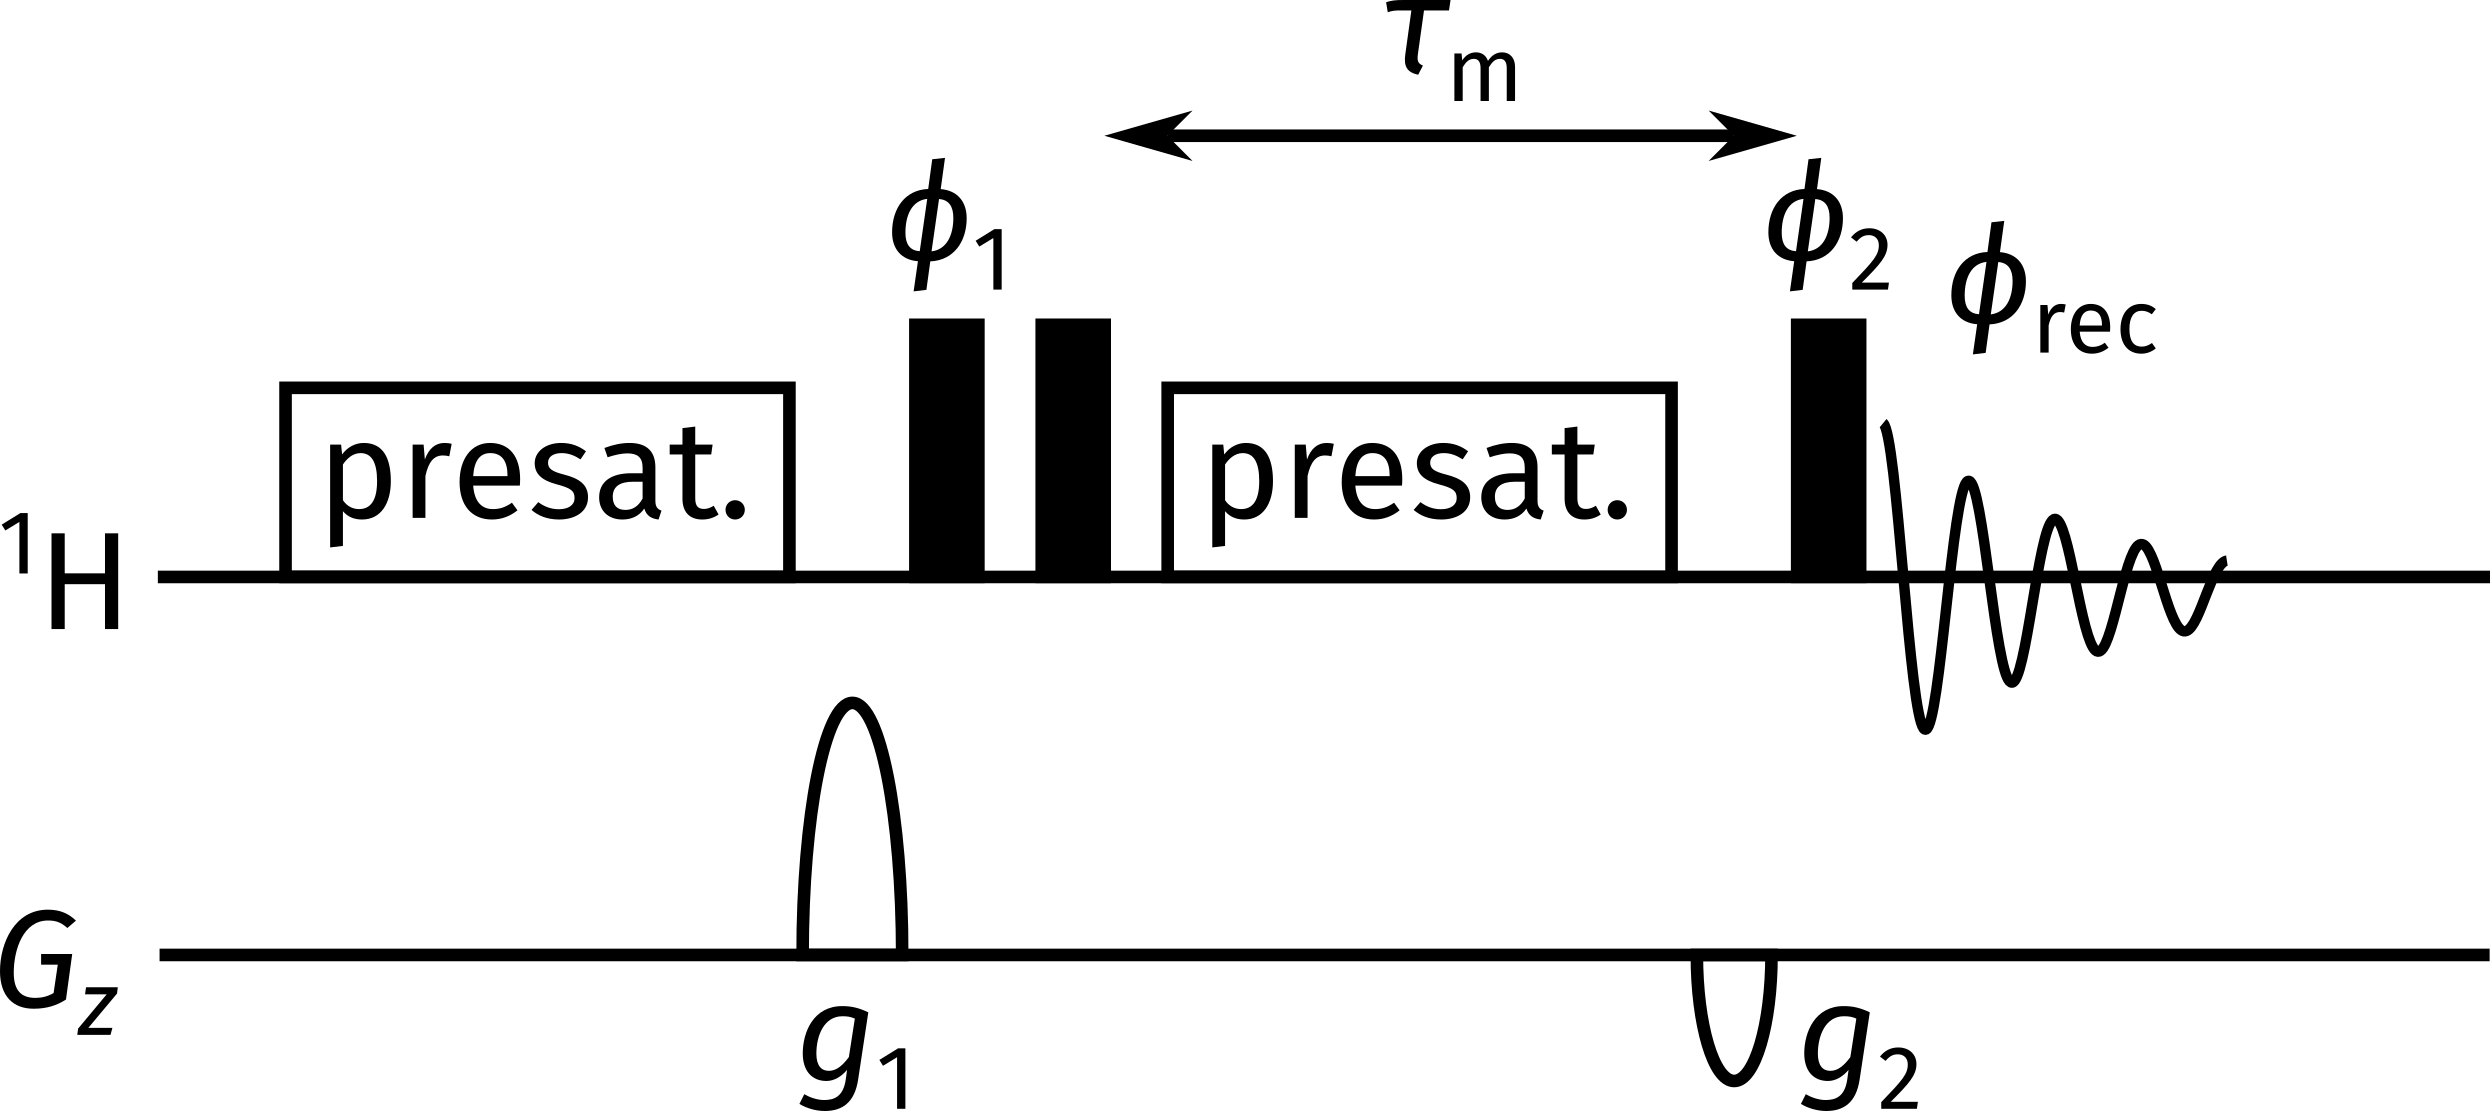
\includegraphics[draft=false]{pp/noesygppr1d.png}%
    \caption[1D NOESY pulse sequence for water suppression]{
        1D NOESY pulse sequence used for water suppression.
        Presaturation of the water resonance is applied during the recovery delay as well as the NOE mixing time.
        Phase cycling is performed with $\phi_1 = (x, -x)$, $\phi_2 = (x, x, -x, -x, y, y, -y, -y)$, and $\phi_\text{rec} = (x, -x, -x, x, y, -y, -y, y)$.
        Gradient amplitudes are $(g_1, g_2) = (50\%, -10\%)$.
        Boxes labelled with `presat.' indicates periods of weak presaturation.
    }
    \label{fig:poise_solvsupp_pulseq}
\end{figure}


\subsubsection{Optimisation setup}

In a similar style to the PSYCHE optimisations (\cref{subsec:poise__psyche}), a series of optimisations with increasing numbers of parameters were run.
However, in this case, the cost function is far easier to construct and far less noisy: we can simply integrate the water peak, which was defined to be the region of the spectrum between 4.65 and \SI{4.75}{\ppm}, and use that (or its absolute value) as the cost function.
In practice, because the phase of the water peak can vary rather unpredictably, I preferred to reuse the sum-of-squares cost function $f_\text{sos}$ (\cref{eq:sos_cost_function}).
Squaring each point of the spectrum not only accounts for the possible sign changes, but also more strongly penalises intense absorption-mode water peaks which are more likely to obscure nearby peaks.

One drawback of the water suppression optimisation is that the phase cycle of the 1D NOESY is integral to its performance: thus, several scans must be used for a reliable cost function to be obtained, making for relatively long optimisations.
In this case, I used \texttt{DS=2} and \texttt{NS=4}.

A sample of rodent urine in \ch{D2O} was used, kindly provided by Abi Yates and Fay Probert (both University of Oxford).



\subsubsection{Optimisation results}

As before, I first provide a `summary' table comparing the optimisations with different numbers of parameters (\cref{tbl:poise_solvsupp_summary}).
From this, we see a similar story to before, in that optimising more parameters takes more time but leads to larger decreases in the cost function.
Individual details of each set of optimisations are given in \cref{tbl:poise_solvsupp1p,tbl:poise_solvsupp2p,tbl:poise_solvsupp3p,tbl:poise_solvsupp4p}.

The corresponding spectra post-optimisation are shown in \cref{fig:poise_solvsupp_spec}.
Clearly, the optimisations succeed in reducing the size of the water peak, especially the four-parameter optimisation.
However, perhaps equally importantly, the doublet at \SI{4.56}{\ppm} is unaffected by the optimisation.
Since the cost function does not actually check for the retention of peaks outside the target window, it is in principle possible that the optimisation will converge to parameters which achieve excellent water suppression but also cause nearby peaks to be lost.
This possibility is averted here by setting a conservative upper bound of \SI{55}{\Hz} on the presaturation power $k$: this avoids inadvertently saturating nearby resonances.

In fact, it may be justifiable in this case to run a long, four-parameter optimisation (which takes around 30 minutes), especially if many samples are to be run using the same optimised water suppression parameters.
However, for more routine usage, it is probably preferable to limit the number of parameters being optimised to two.


\begin{table}
    \centering
    \begin{tabular}{cccccccc}
        \toprule
         & \multicolumn{3}{c}{Aggregated results from all runs} & \multicolumn{4}{c}{Parameters from best optimum} \\
        Description & $f_\mathrm{sos} / 10^{18}$ & FEs & Time (\si{\s}) & $\nu_\text{tx}$ (\si{\Hz}) & $k$ (\si{\Hz}) & $\taum$ (\si{\s}) & $\taur$ (\si{\s}) \\
        \hline
        Initial point & 14.7         & --     & --         & (1880.61) & (50.0) & (0.100) & (2.00) \\
        1 parameter   & 1.85--2.49   & 6--12  & 259--520   & 1880.41   & (50.0) & (0.100) & (2.00) \\
        2 parameters  & 1.21--9.68   & 9--21  & 390--911   & 1880.20   & 51.94  & (0.100) & (2.00) \\
        3 parameters  & 1.24--4.20   & 19--26 & 825--1128  & 1879.90   & 47.79  & 0.118   & (2.00) \\
        4 parameters  & 0.165--1.65  & 25--53 & 1143--2314 & 1881.10   & 53.28  & 0.150   & 3.00 \\
        \hline
    \end{tabular}
    \caption[Overview of all water suppression optimisations]{
        Summary of optimisations on 1D NOESY / presaturation pulse sequence for water suppression.
        Parameters in parentheses were not optimised and were simply carried over from the initial point.
        A detailed breakdown of the results by algorithm, as well as the POISE routines used, are described in \cref{tbl:poise_solvsupp1p,tbl:poise_solvsupp2p,tbl:poise_solvsupp3p,tbl:poise_solvsupp4p}.
        \datacode{4P-210620}
    }
    \label{tbl:poise_solvsupp_summary}
\end{table}

\begin{figure}[htb]
    \centering
    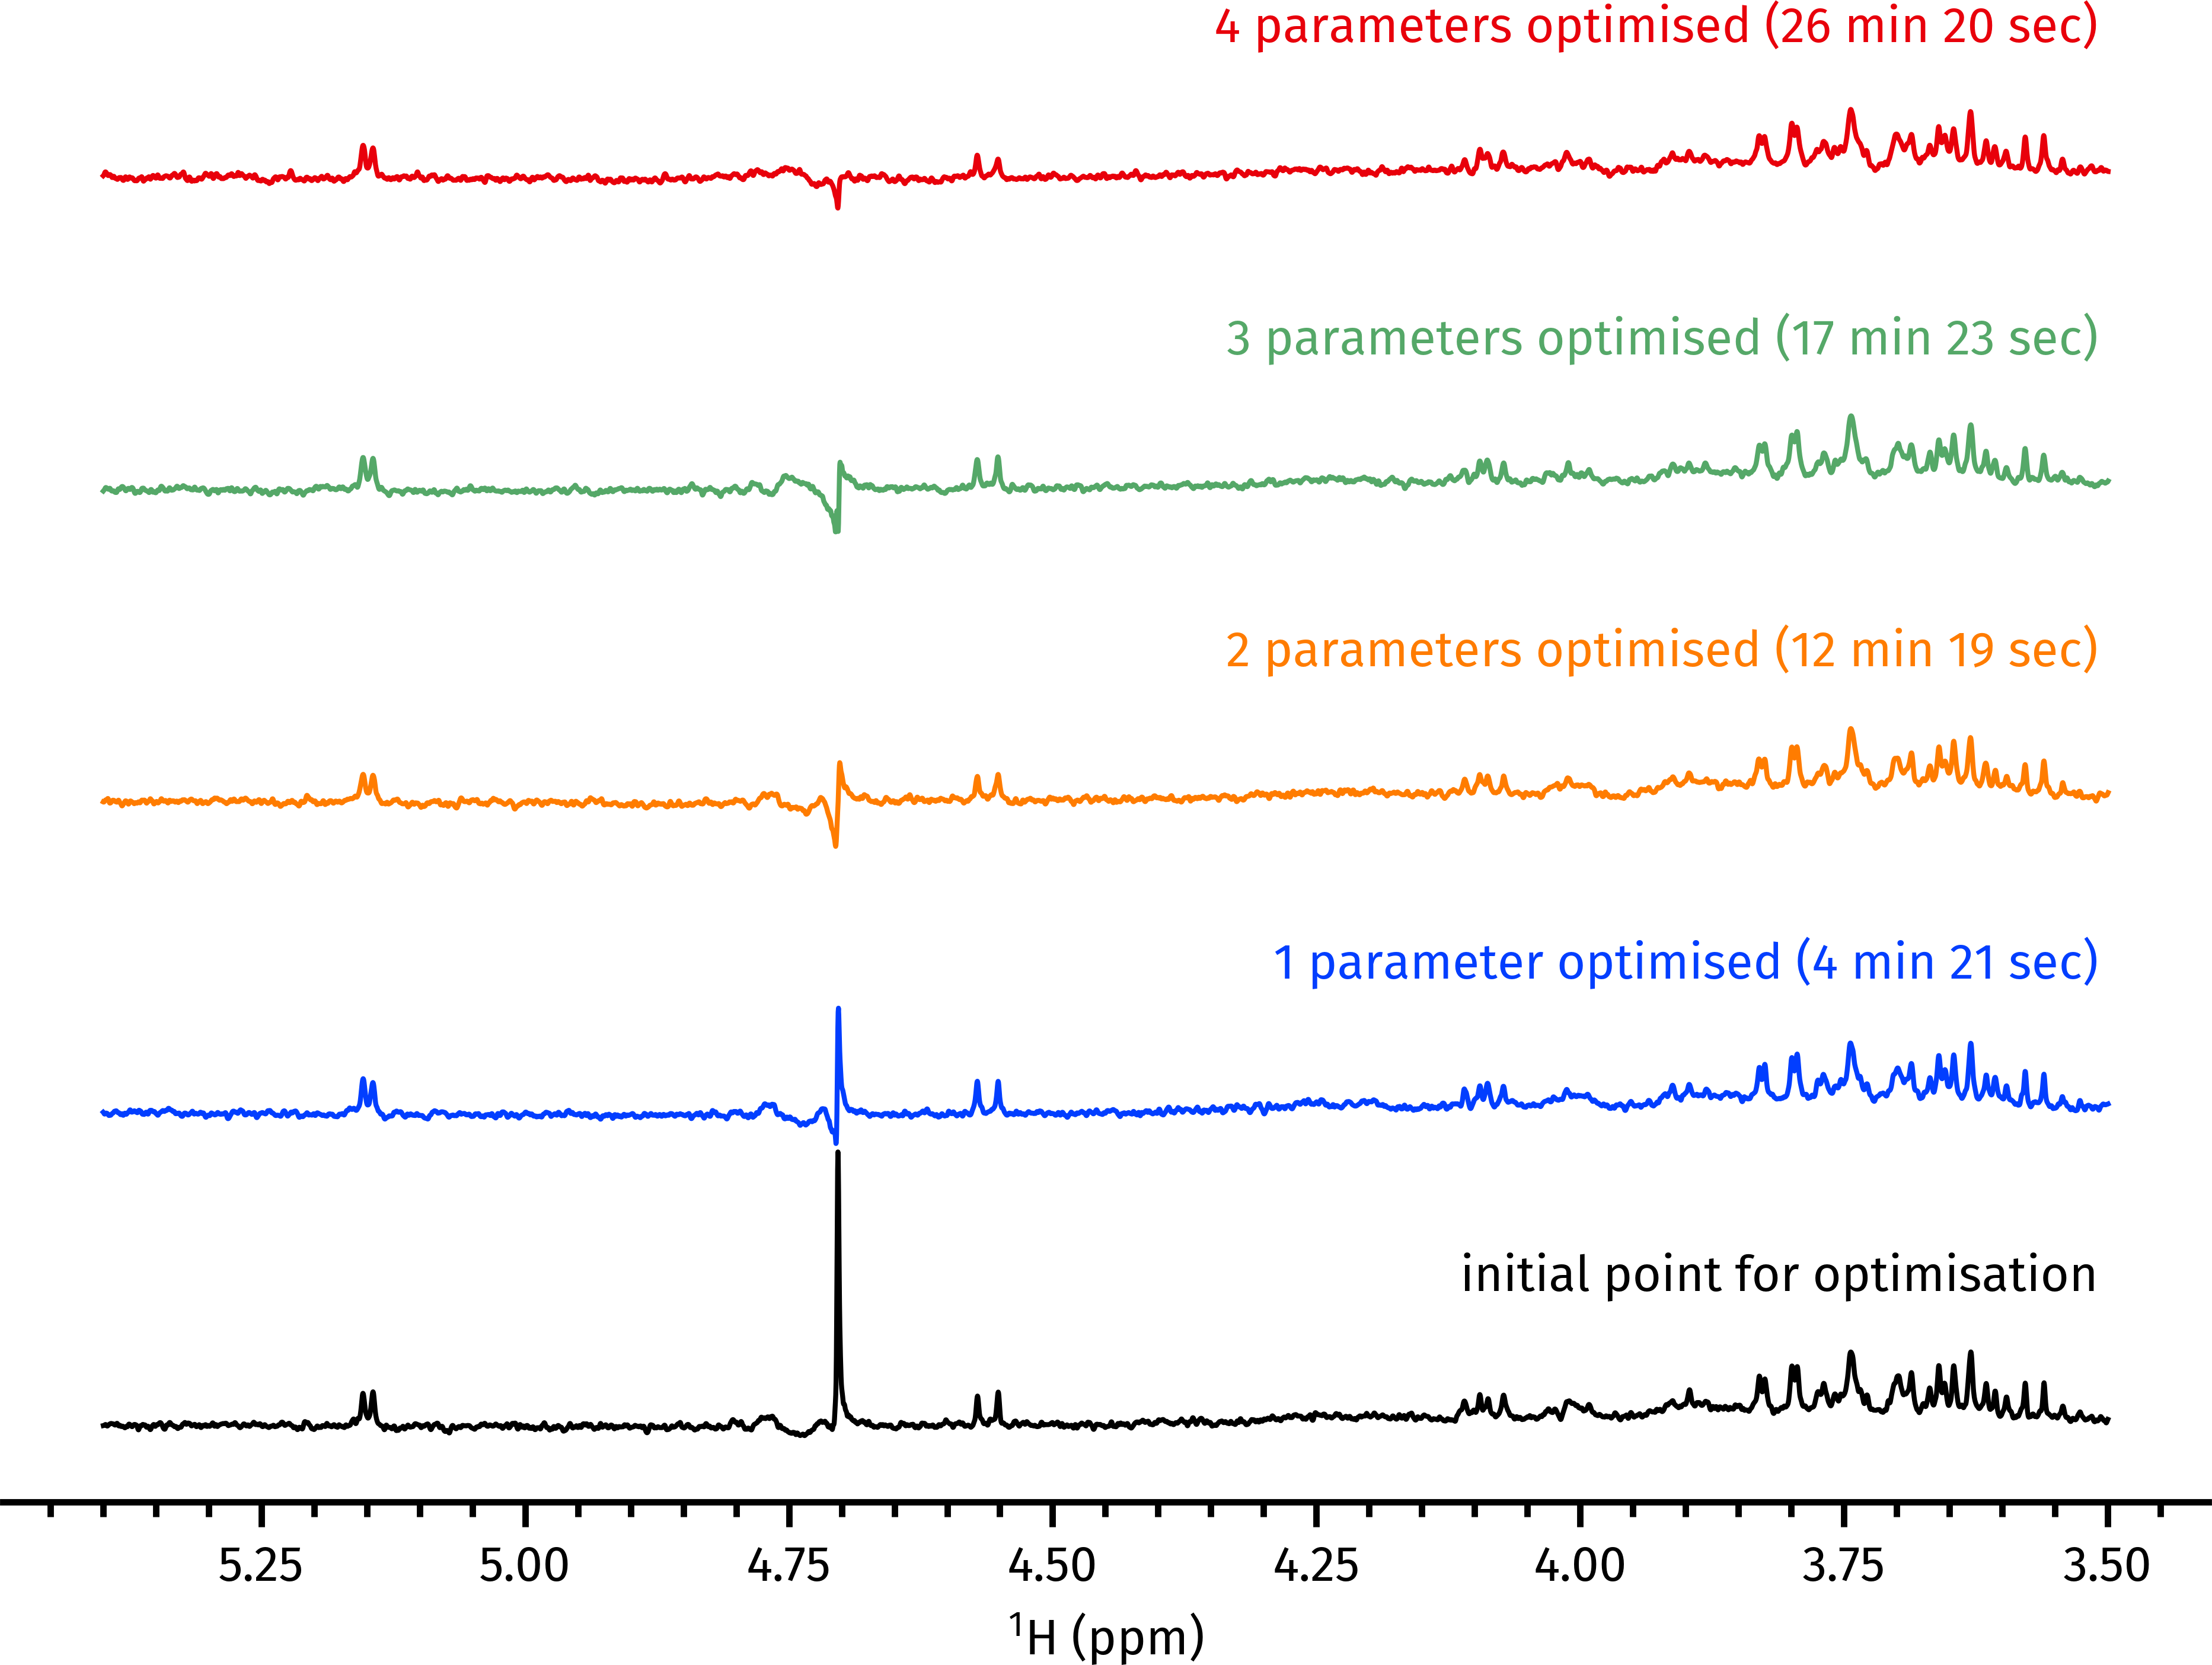
\includegraphics[draft=false]{poise/solvsupp_spec.png}
    \caption[1D NOESY spectra of rodent urine sample before and after optimisation]{
        Insets of 1D NOESY spectra acquired using optimised parameters from each set of optimisations in \cref{tbl:poise_psyche_summary}; the time required to obtain the optimised parameters is also indicated for each spectrum.
        The sample used was rodent urine in \ch{D2O}.
        Note that, for the 3- and 4-parameter optimisations, the best optimum from the 15 runs (i.e.\ the optima listed in \cref{tbl:poise_solvsupp_summary}) was used to acquire the spectra shown here.
        However, this was not the case for the 2-parameter optimisation: I (inexplicably) used a different optimum.
        This was probably an oversight on my part.
        Nevertheless, it does not affect any of the conclusions drawn here.
        \datacode{4P-210620}
    } \label{fig:poise_solvsupp_spec}
\end{figure}

\begin{table}
    \hbadness=10000
    \centering
    \begin{tabular}{ccccc}
        \toprule
        Entry & Algorithm & Optimum found (\si{\Hz}) & FEs    & Time taken (\si{\s}) \\
        \midrule
        1     & NM        & 1880.24--1880.49         & 10--12 & 436--519             \\
        2     & MDS       & 1880.24--1880.36         & 12     & 518--520             \\
        3     & BOBYQA    & 1880.34--1880.47         & 6--7   & 259--303             \\
        \bottomrule
    \end{tabular}
    \caption{
        Water suppression 1-parameter (transmitter offset) optimisations.
        The POISE routine used was: \mintinline[breaklines]{json}{{"name": "solvsupp1", "pars": ["o1"], "lb": [1870.61], "ub": [1890.61], "init": [1880.61], "tol": [0.2], "cf": "zerorealint_squared", "au": "poise_1d_noapk"}}.
        \datacode{4P-210620}
    }
    \label{tbl:poise_solvsupp1p}
\end{table}

\begin{table}
    \hbadness=10000
    \centering
    \begin{tabular}{ccccccc}
        \toprule
              &           & \multicolumn{3}{c}{Best optimum found} & \multicolumn{2}{c}{Aggregated results} \\
                            \cmidrule(lr){3-5}                       \cmidrule(lr){6-7}
        Entry & Algorithm & $\nu_\text{tx}$ (\si{\Hz}) & $k$ (\si{\Hz}) & $f_\text{sos} / 10^{18}$ & FEs    & Time (\si{\s}) \\
        \midrule
        1     & NM        & 1880.20                    & 51.94          & 1.209                    & 17--21 & 737--911       \\
        2     & MDS       & 1880.85                    & 50.81          & 2.600                    & 15     & 649--652       \\
        3     & BOBYQA    & 1881.12                    & 50.03          & 2.887                    & 9--14  & 390--608       \\
        \bottomrule
    \end{tabular}
    \caption{
        Water suppression 2-parameter (transmitter offset and presaturation power) optimisations.
        The POISE routine used was: \mintinline[breaklines]{json}{{"name": "solvsupp2", "pars": ["o1", "cnst20"], "lb": [1870.61, 10.0], "ub": [1890.61, 55.0], "init": [1880.61, 50.0], "tol": [0.2, 2.5], "cf": "zerorealint_squared", "au": "poise_1d_noapk"}}.
        \datacode{4P-210620}
    }
    \label{tbl:poise_solvsupp2p}
\end{table}

\begin{table}
    \hbadness=10000
    \centering
    \begin{tabular}{cccccccc}
        \toprule
              &           & \multicolumn{4}{c}{Best optimum found} & \multicolumn{2}{c}{Aggregated results} \\
                            \cmidrule(lr){3-6}                       \cmidrule(lr){7-8}
        Entry & Algorithm & $\nu_\text{tx}$ (\si{\Hz}) & $k$ (\si{\Hz}) & $\taum$ (\si{\ms}) & $f_\text{sos} / 10^{18}$ & FEs    & Time (\si{\s}) \\
        \midrule
        1     & NM        & 1879.90                    & 47.79          & 117.7              & 1.238                    & 23--26 & 1002--1128     \\
        2     & MDS       & 1882.79                    & 52.95          & 49.91              & 1.843                    & 24--25 & 1034--1080     \\
        3     & BOBYQA    & 1881.85                    & 52.14          & 134.7              & 1.738                    & 19--26 & 825--1133      \\
        \bottomrule
    \end{tabular}
    \caption{
        Water suppression 3-parameter (transmitter offset, presaturation power, and mixing time) optimisations.
        The POISE routine used was: \mintinline[breaklines]{json}{{"name": "solvsupp3", "pars": ["o1", "cnst20", "d8"], "lb": [1870.61, 10.0, 0.010], "ub": [1890.61, 55.0, 0.150], "init": [1880.61, 50.0, 0.100], "tol": [0.2, 2.5, 0.010], "cf": "zerorealint_squared", "au": "poise_1d_noapk"}}.
        \datacode{4P-210620}
    }
    \label{tbl:poise_solvsupp3p}
\end{table}

\begin{table}
    \hbadness=10000
    \centering
    \begin{tabular}{ccccccccc}
        \toprule
              &           & \multicolumn{5}{c}{Best optimum found} & \multicolumn{2}{c}{Aggregated results} \\
                            \cmidrule(lr){3-7}                       \cmidrule(lr){8-9}
        Entry & Algorithm & $\nu_\text{tx}$ (\si{\Hz}) & $k$ (\si{\Hz}) & $\taum$ (\si{\ms}) & $\taur$ (\si{\s}) & $f_\text{sos} / 10^{18}$ & FEs    & Time (\si{\s}) \\
        \midrule
        1     & NM        & 1880.72                    & 49.73          & 110.6              & 1.972             & 1.008                    & 29--40 & 1250--1726     \\
        2     & MDS       & 1882.65                    & 53.41          & 69.46              & 2.137             & 1.199                    & 34--53 & 1487--2314     \\
        3     & BOBYQA    & 1881.10                    & 53.28          & 150.0              & 3.000             & 0.1653                   & 25--40 & 1143--1843     \\
        \bottomrule
    \end{tabular}
    \caption{
        Water suppression 4-parameter (transmitter offset, presaturation power, mixing time, and presaturation duration) optimisations.
        The POISE routine used was: \mintinline[breaklines]{json}{{"name": "solvsupp4", "pars": ["o1", "cnst20", "d8", "d1"], "lb": [1870.61, 10.0, 0.010, 1.0], "ub": [1890.61, 55.0, 0.150, 3.0], "init": [1880.61, 50.0, 0.100, 2.0], "tol": [0.2, 2.5, 0.010, 0.1], "cf": "zerorealint_squared", "au": "poise_1d_noapk"}}.
        \datacode{4P-210620}
    }
    \label{tbl:poise_solvsupp4p}
\end{table}




\subsubsection{Optimisation on a sucrose sample}

The water suppression optimisations shown above were in fact developed and first evaluated on a sample of sucrose in 90\% \ch{H2O}/10\% \ch{D2O}.
This sample is less `interesting' in that there are no resonances close to the water peak, and I also did not perform replicates of each optimisation run (this data never made it into the POISE paper).
Nevertheless, I still believe it is still worth adding the results here, as they demonstrate that the optimisation procedure can be easily applied to different samples.

In this case, the one-parameter optimisation seemed to have no significant effect on the result: this is possibly because the initial value chosen for that single parameter (the transmitter offset) already happened to be an optimum.
However, the two- through four-parameter optimisations all yielded significant improvements in the water suppression (\cref{fig:poise_solvsupp_sucrose_spec}).

\begin{figure}[htb]
    \centering
    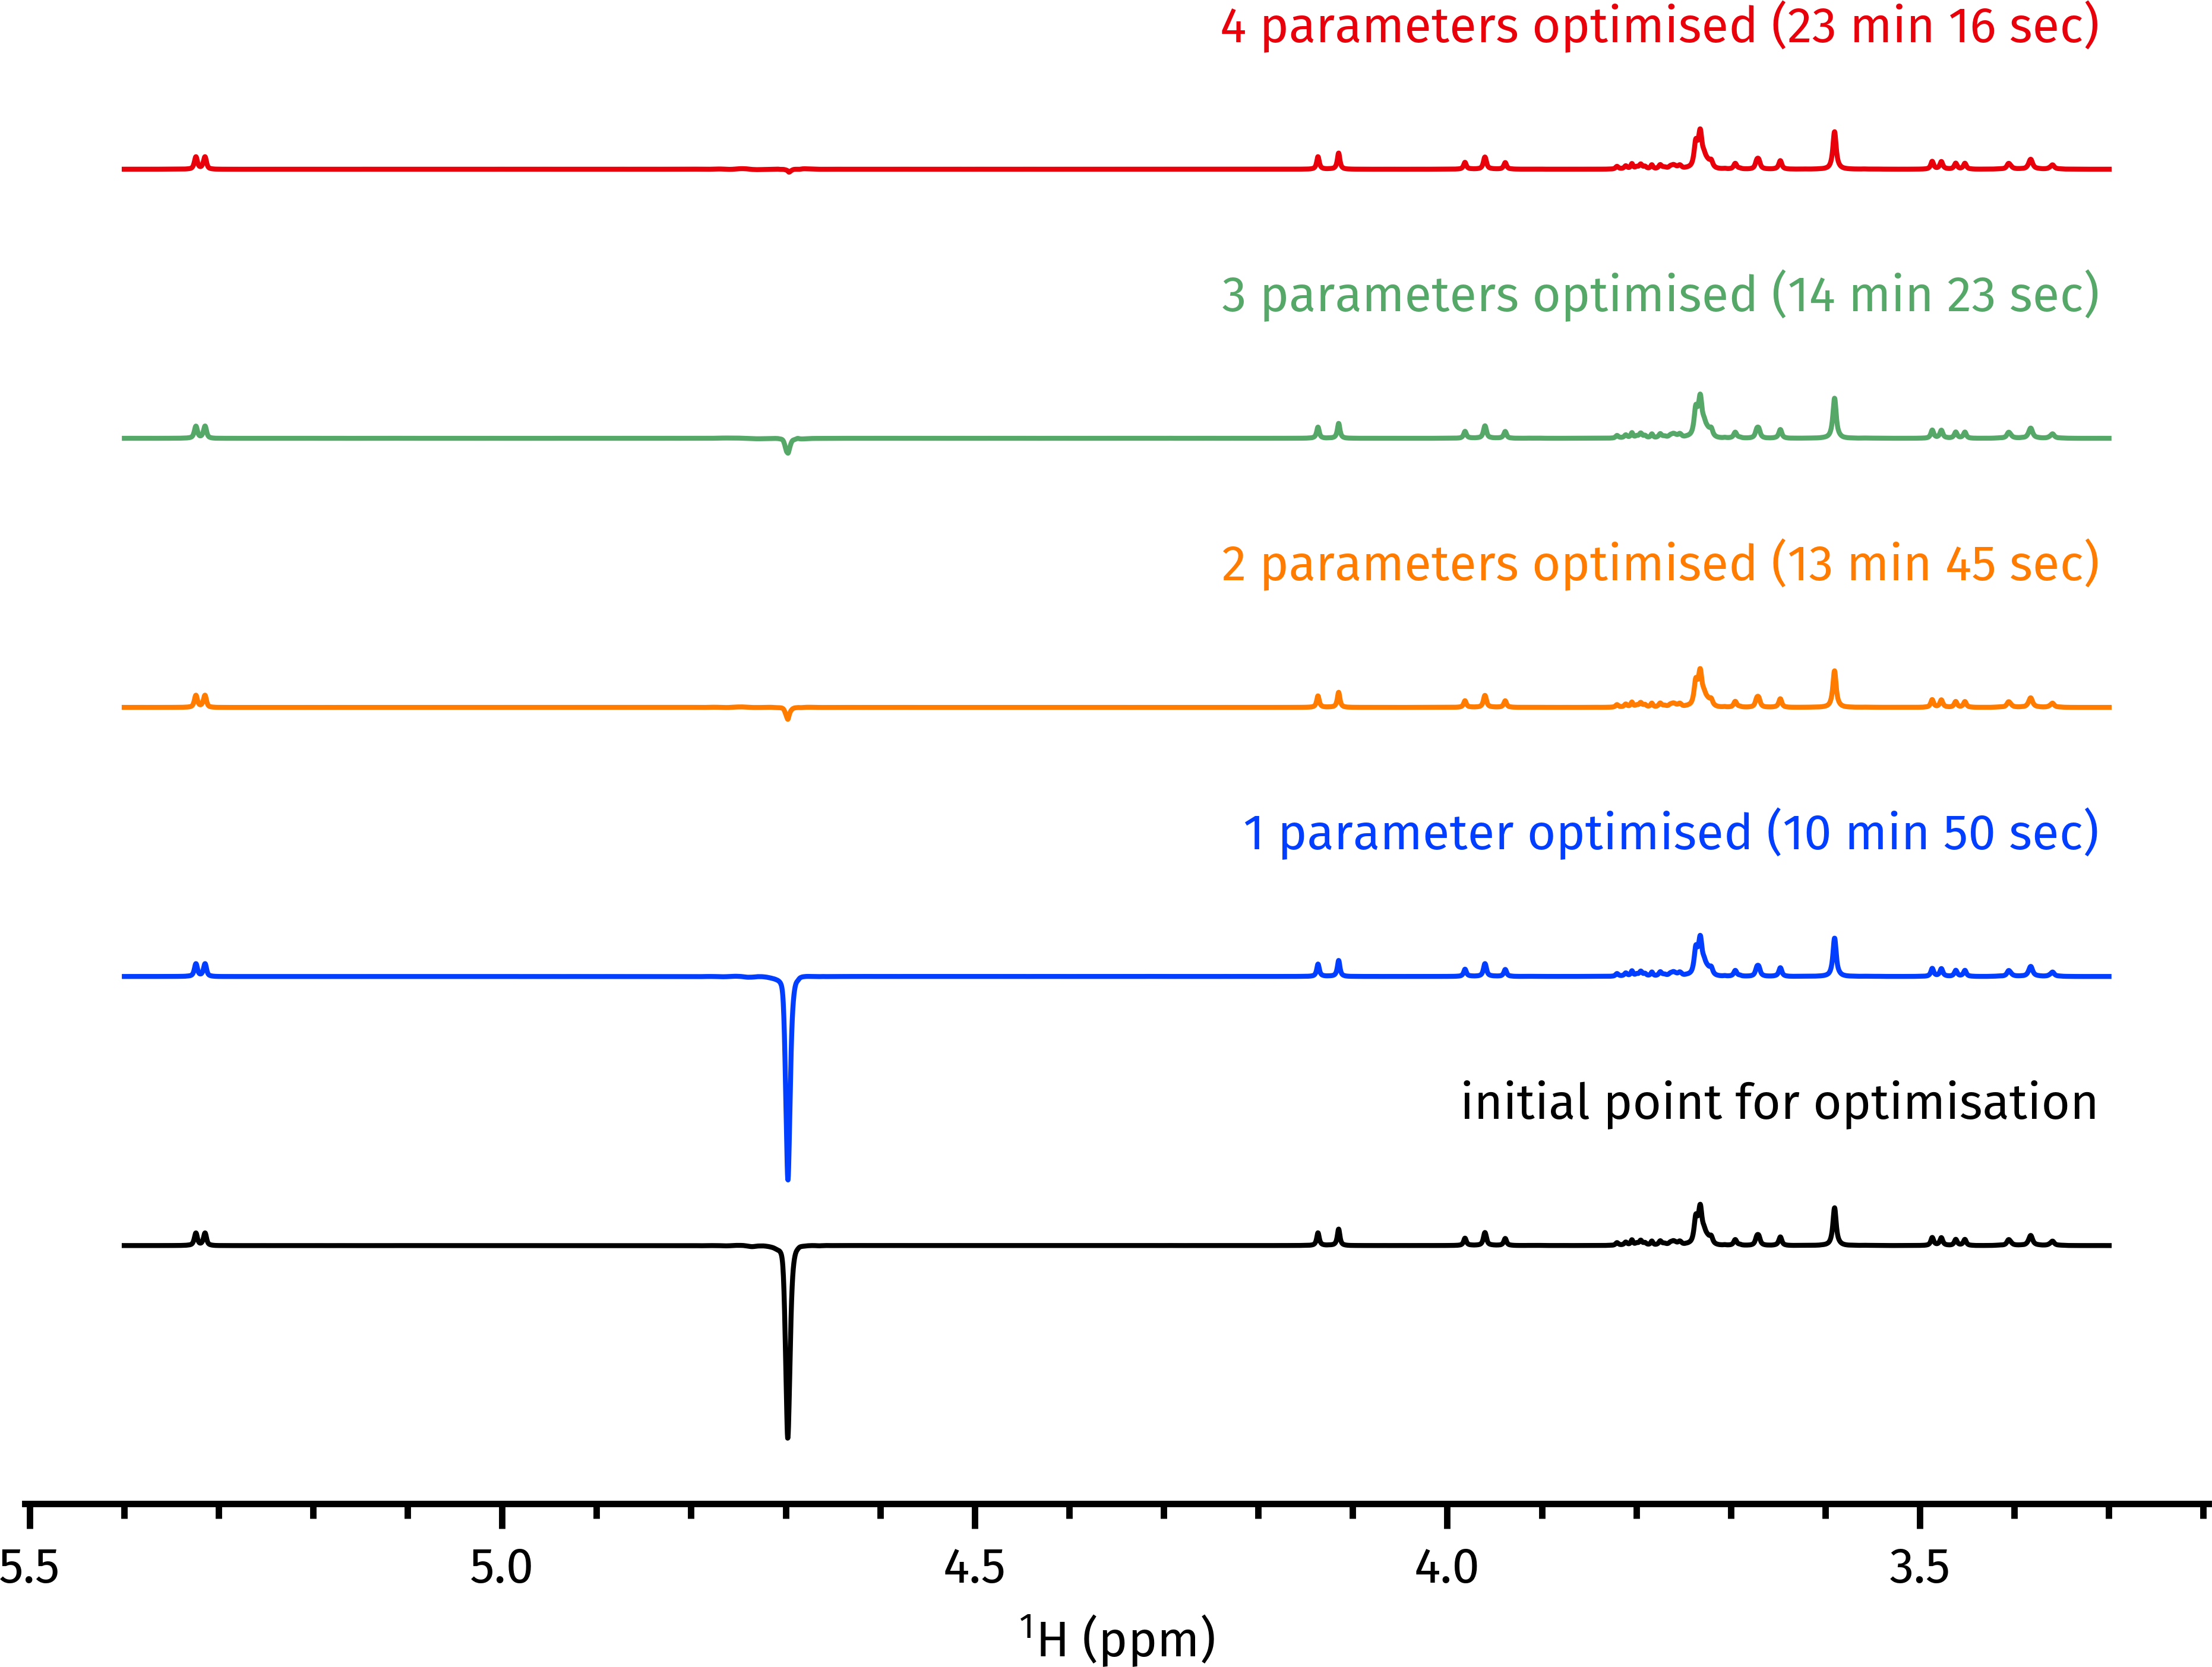
\includegraphics[draft=false]{poise/solvsupp_sucrose_spec.png}
    \caption[1D NOESY spectra of sucrose sample before and after optimisation]{
        Insets of 1D NOESY spectra acquired after optimisation of 1, 2, 3, or 4 parameters (the exact parameters being optimised are the same as in \cref{fig:poise_solvsupp_spec}).
        The sample used was sucrose in 90\% \ch{H2O}/10\% \ch{D2O}.
        The time required to obtain the optimised parameters is also indicated for each spectrum.
        \datacode{4S-210617}
    }
    \label{fig:poise_solvsupp_sucrose_spec}
\end{figure}

\subsection{Diffusion NMR}
\label{subsec:poise__diffusion}

As the final example of a POISE optimisation, I demonstrate its application to \acf{dosy} experiments.\autocite{Johnson1999PNMRS}
DOSY experiments measure molecular diffusion during a delay period, $\Delta$, which is placed between two gradients, such as in the stimulated echo experiment (\cref{fig:poise_dosy_pulseq_ste}), or the bipolar pulse pair version (\cref{fig:poise_dosy_pulseq_stebpp}) which uses opposing gradients to refocus the lock signal during the sequence.
In these sequences, the first `encoding' gradient (or set thereof) imparts a spatially-dependent phase, which---in the absence of diffusion---is perfectly refocused by the second `decoding' gradient (or set thereof).
However, if diffusion is present, this refocusing is not complete, leading to signal attenuation which is described by the Stejskal--Tanner equation:
\begin{equation}
    \label{eq:stejskal_tanner_again}
    I(G) = I(0) \exp\left[-(\gamma\delta G)^2 D \Delta'\right].
\end{equation}
Here, $G$ is the amplitude of the encoding and decoding gradients, $\delta$ the duration of the gradients, and $\Delta'$ is a corrected diffusion delay.

\begin{figure}[htb]
    \centering
    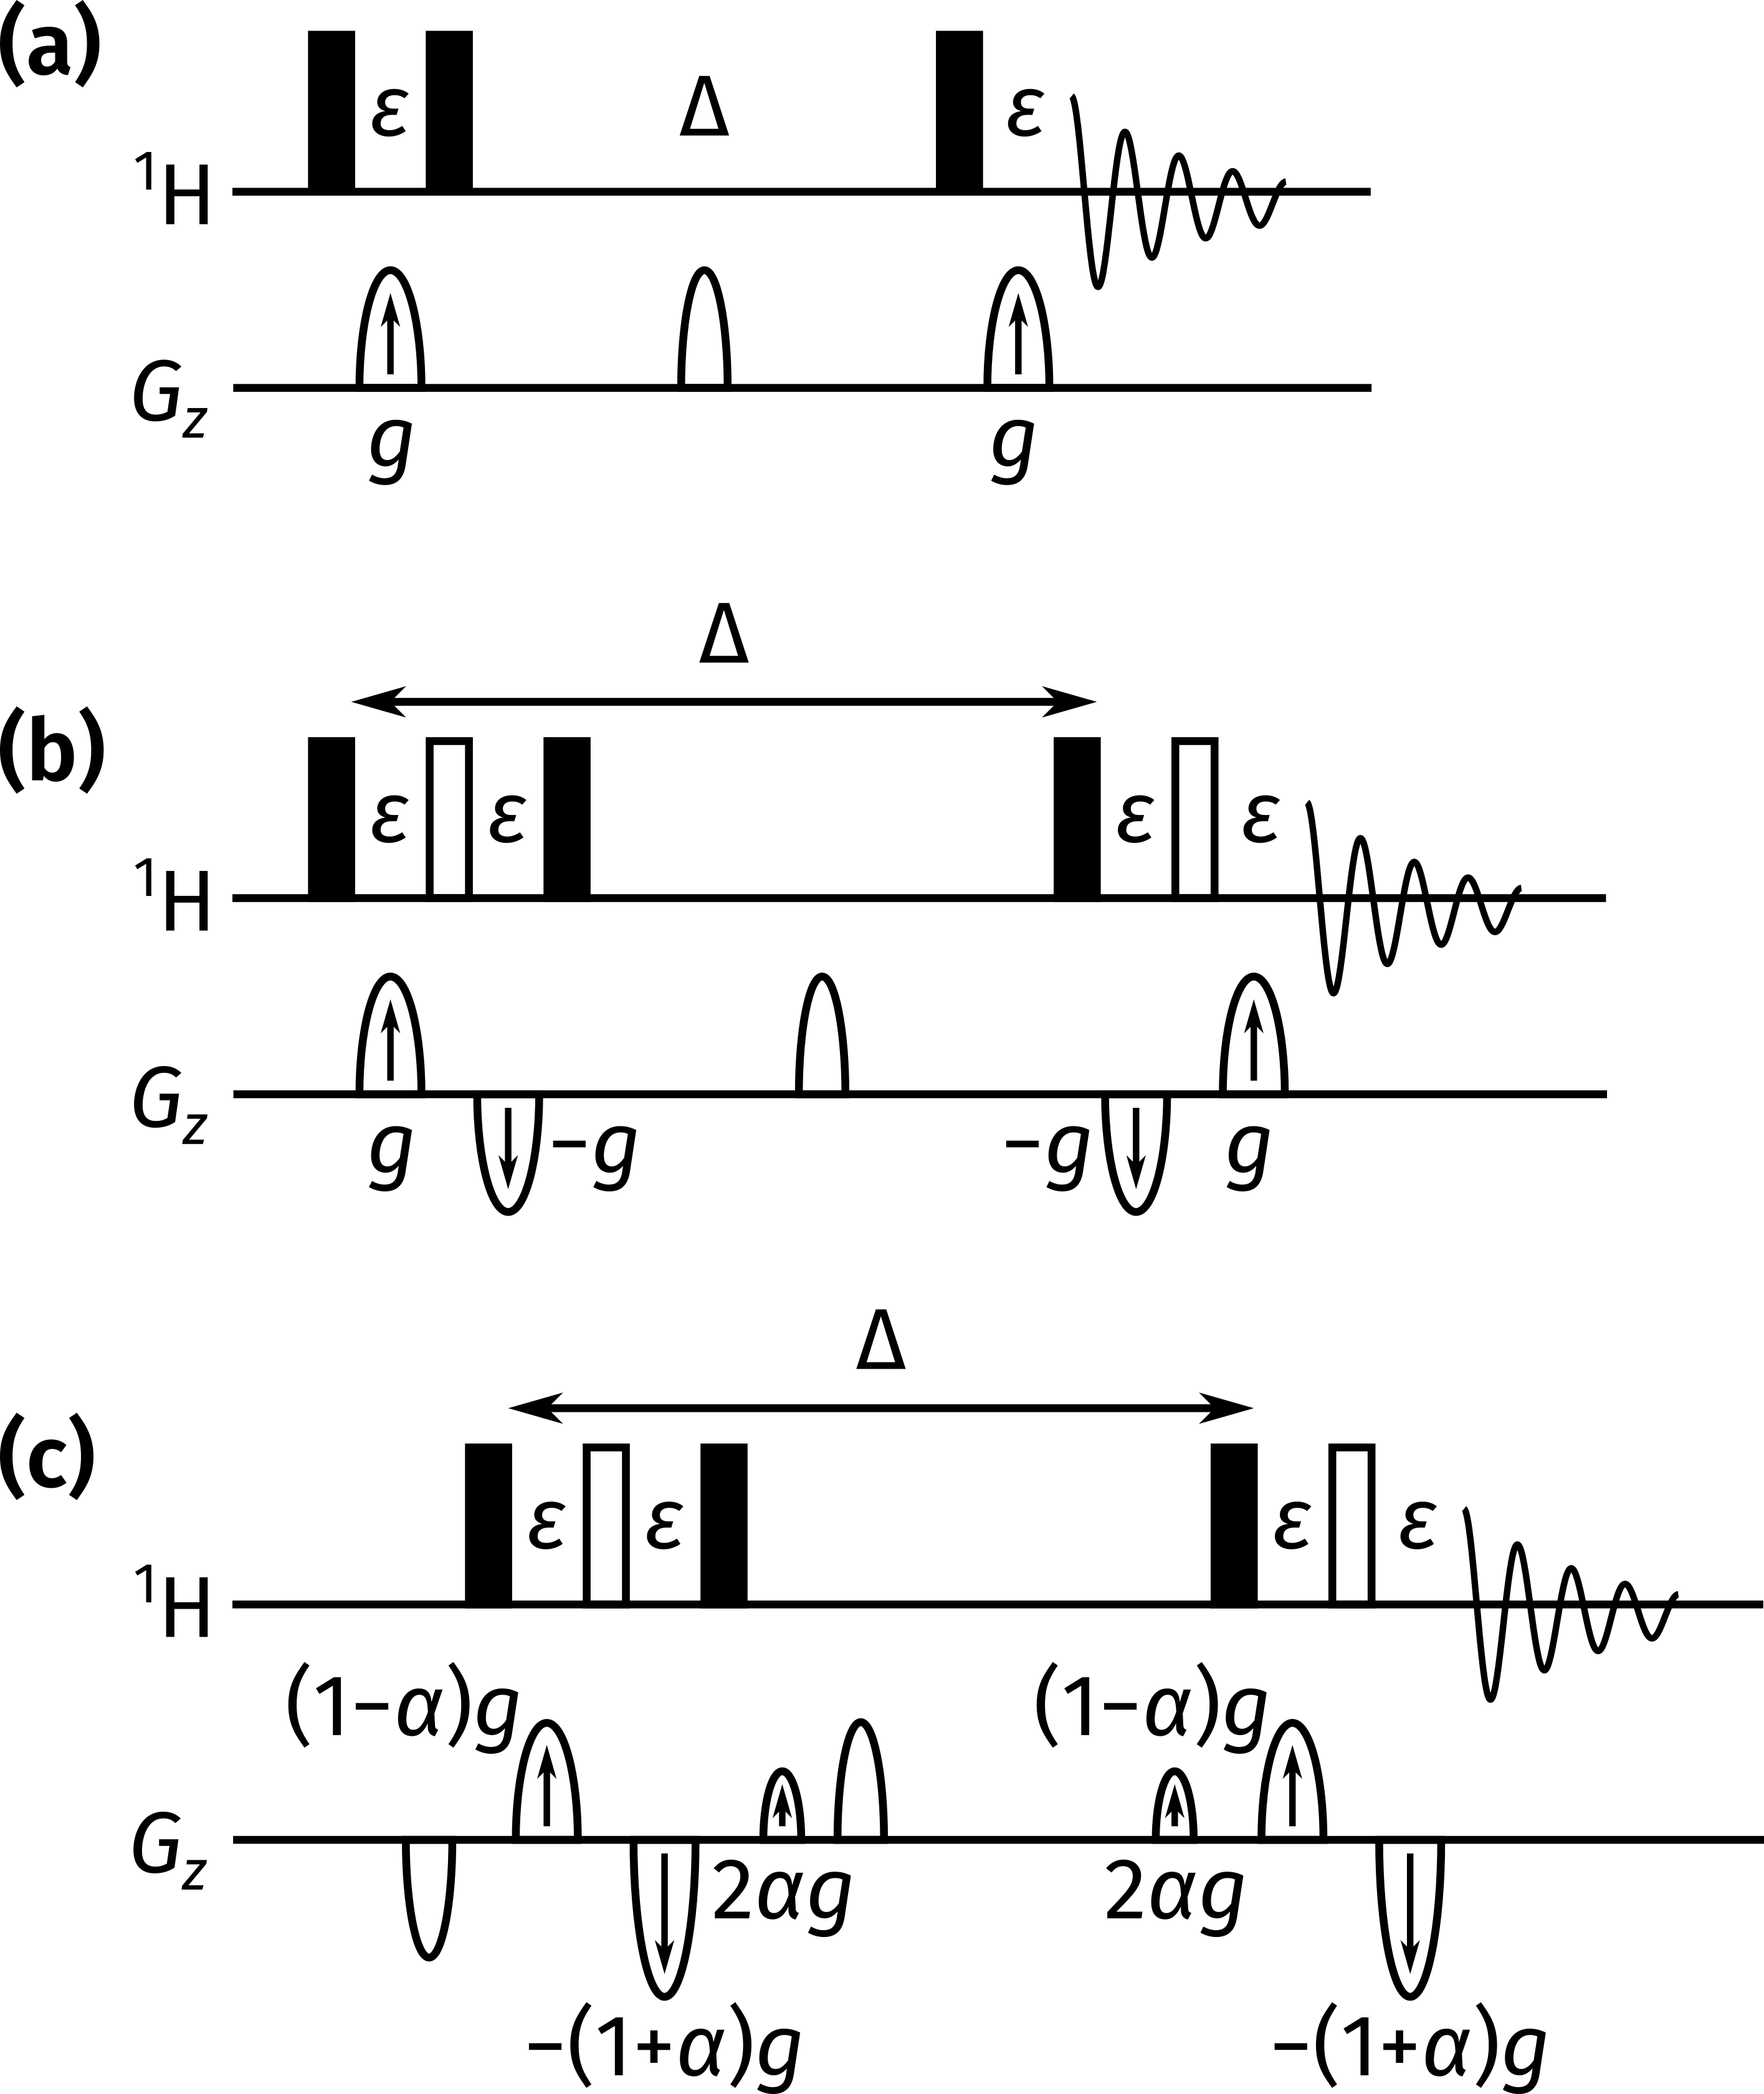
\includegraphics[]{pp/poise/dosy.png}
    {\phantomsubcaption\label{fig:poise_dosy_pulseq_ste}}
    {\phantomsubcaption\label{fig:poise_dosy_pulseq_stebpp}}
    {\phantomsubcaption\label{fig:poise_dosy_pulseq_oneshot}}
    \caption[Selection of DOSY pulse sequences]{
        \textbf{(\subref{fig:poise_dosy_pulseq_ste})} Stimulated echo DOSY pulse sequence. The diffusion-encoding and -decoding gradients, whose amplitudes are incremented, are marked with arrows.
        \textbf{(\subref{fig:poise_dosy_pulseq_stebpp})} Stimulated echo bipolar pulse pair DOSY pulse sequence.
        \textbf{(\subref{fig:poise_dosy_pulseq_oneshot})} Oneshot DOSY pulse sequence.
    }
    \label{fig:poise_dosy_pulseq}
\end{figure}

Typically, diffusion experiments are measured in a 2D method where each increment is measured with a different gradient amplitude $G$.
The value of $D$ can then be extracted through various means, most simply an exponential fitting of the measured intensities $I(G)$ for single species (or distinct species which do not overlap).
In order to minimise the uncertainty in the calculated diffusion coefficients, the parameters $\Delta$ and $\delta$, as well as the range of gradient amplitudes used (and possibly also their distribution), should be chosen in order to yield a diffusion profile of the form in \cref{fig:diffusion_sim_ok}.
Generally, the last increment (acquired using the maximum gradient strength, $G_\text{max}$ should have an attenuation of 5--35\%\footnote{Recommendations tend to vary.} when compared against the first increment (acquired with the minimum gradient amplitude, $G_\text{min}$, which may be 0).
Traditionally, this is done `by hand' by acquiring individual increments of the 2D diffusion experiment, checking the attenuation, and adjusting the parameters accordingly.\autocite{Johnson1999PNMRS,Claridge2016}

\begin{figure}[htb]
    \centering
    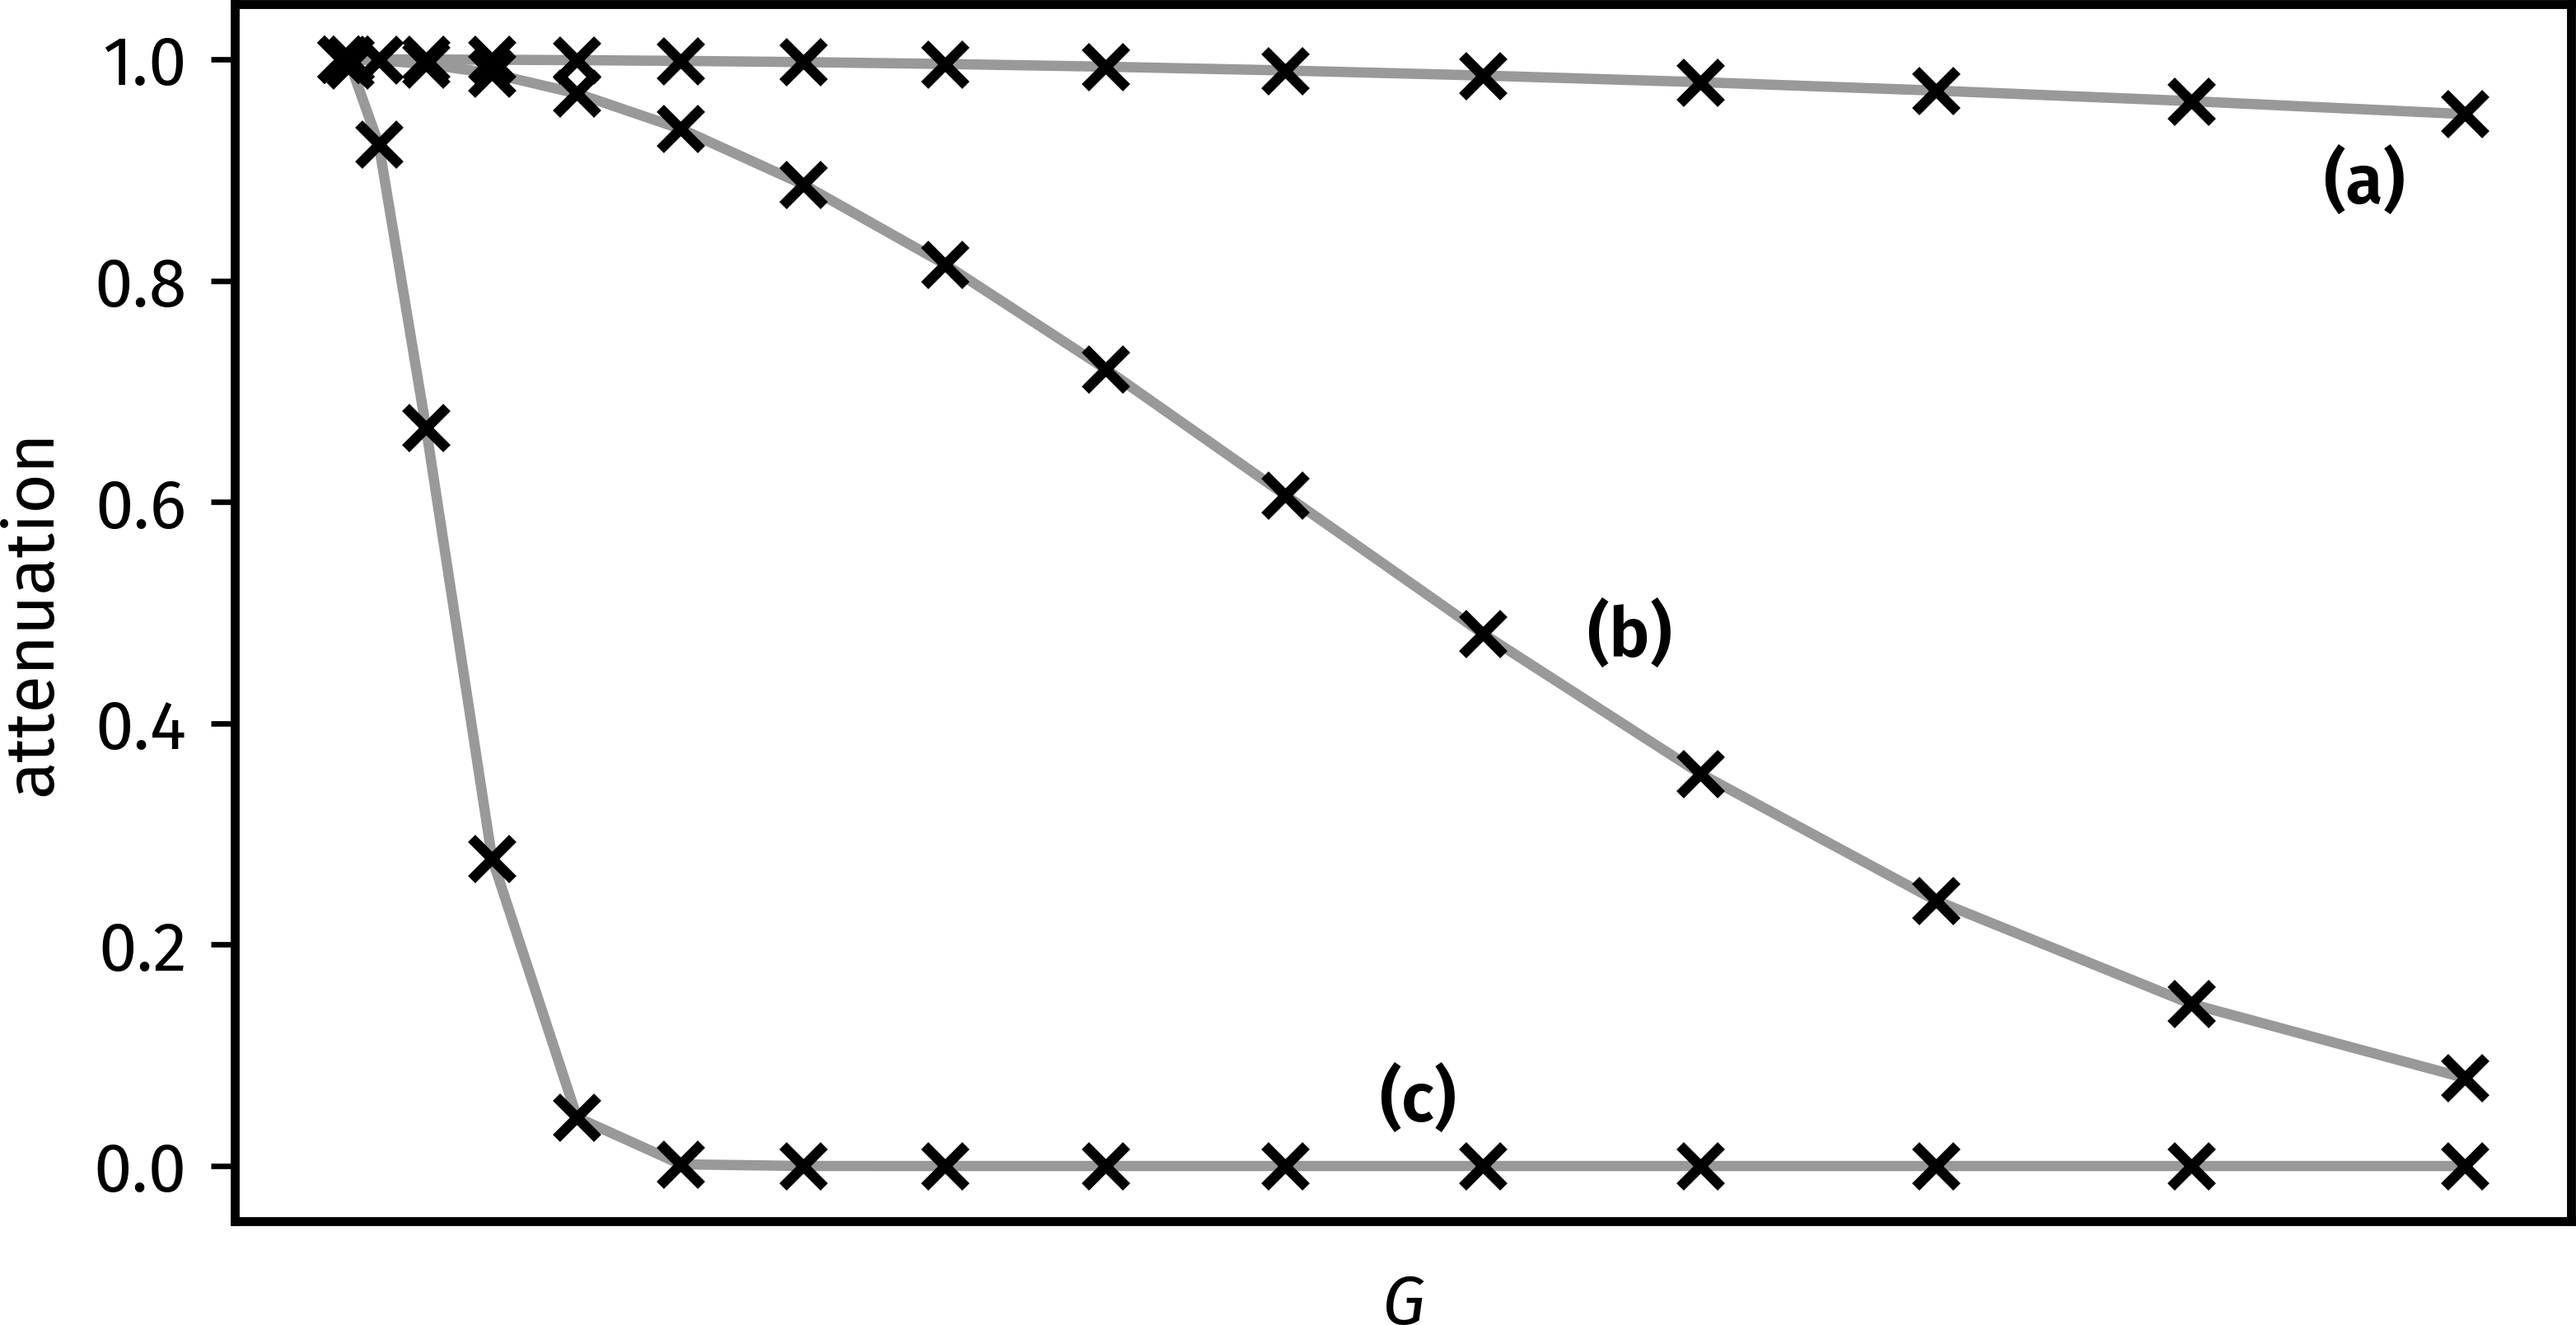
\includegraphics[]{poise/diffusion_sim.png}%
    {\phantomsubcaption\label{fig:diffusion_sim_weak}}%
    {\phantomsubcaption\label{fig:diffusion_sim_ok}}%
    {\phantomsubcaption\label{fig:diffusion_sim_strong}}%
    \caption[Simulated diffusion profiles for slow, intermediate, and rapid diffusion]{
        Simulated diffusion profiles for species with different diffusion rates.
        \textbf{(\subref{fig:diffusion_sim_weak})} A slowly diffusing species: insufficient attenuation is observed with the given parameters, meaning that generally $\Delta$ or $\delta$ need to be increased.
        \textbf{(\subref{fig:diffusion_sim_ok})} An `ideal' diffusion profile where attenuation is neither too little or too much.
        \textbf{(\subref{fig:diffusion_sim_strong})} A rapidly diffusing species, for which complete attenuation is already accomplished using low gradient amplitudes. This generally suggests that $\Delta$ or $\delta$ need to be decreased, or a new gradient ramp calculated.
    }
    \label{fig:diffusion_sim}
\end{figure}

This task could of course be delegated to a computer programme such as POISE.
We \textit{could} simply tackle it head-on by optimising all of $\Delta$, $\delta$, and $G_\text{max}$ at once (assuming that $G_\text{min}$ is fixed); however, this is actually rather inefficient.
Firstly, we previously saw that multiple-parameter optimisations took a longer time than the corresponding one-parameter optimisations.
However, on top of that, it is often not even necessary to change all three parameters: the Stejskal--Tanner equation shows that the diffusion attenuation is controlled only by the overall \textit{product} $\delta^2 G_\text{max}^2 \Delta'$.
Thus, at least to a first approximation, the individual values of $\Delta$, $\delta$, and $G_\text{max}$ do not actually matter.
It makes sense to fix two of these and optimise one parameter, only changing the other two if necessary.

It should be mentioned here that obtaining \textit{accurate} values of $D$ requires careful consideration of various factors such as the exact DOSY sequence and gradient shapes used\autocite{Sinnaeve2012CMR}, peak overlap\autocite{Antalek1996JACS,Windig1997CILS,Nilsson2006AC,Nilsson2008AC,Colbourne2011JACS}, and convection\autocite{Swan2015JMR,Barbosa2016RSCA}.
This may influence the type of processing which is chosen for extraction of diffusion coefficients.
However, these issues are not our concern here: the role of POISE is only to find a good set of acquisition parameters such that the resulting data is amenable towards further processing.



\subsubsection{Optimisation setup}

The overall strategy for this `optimisation' can be briefly summarised in a flowchart (\cref{fig:dosy_flowchart}).
Note that this is \textit{not} a classic optimisation which falls nicely into the POISE workflow (\cref{fig:poise_flowchart}): thus, the entire procedure cannot simply be summarised into one POISE routine.
However, it does contain two optimisation subproblems: one to adjust $\Delta$ if necessary, and one to find $G_\text{max}$.
We can therefore create a wrapper script for the overall procedure (here called \texttt{dosy\_opt.py}, which invokes POISE to solve the two individual subproblems.
This approach is made possible by the command-line interface of POISE, which allows for the creation and execution of optimisation routines.
We also exploit the fact that during the optimisation, POISE stores the value of the cost function as the \texttt{TI} parameter in TopSpin.
This fact is often irrelevant as the value of the cost function is not often of great interest, but proves to be handy in this particular instance as it allows POISE to pass information back to the wrapper script.
Previously, we explored situations where the functionality of POISE could be extended from \textit{within}, e.g.\ by invoking different scripts in its acquisition AU programme.
In this case, we are going in the other direction, allowing POISE to be incorporated in other scripts.

\begin{figure}[htb]
    \centering
    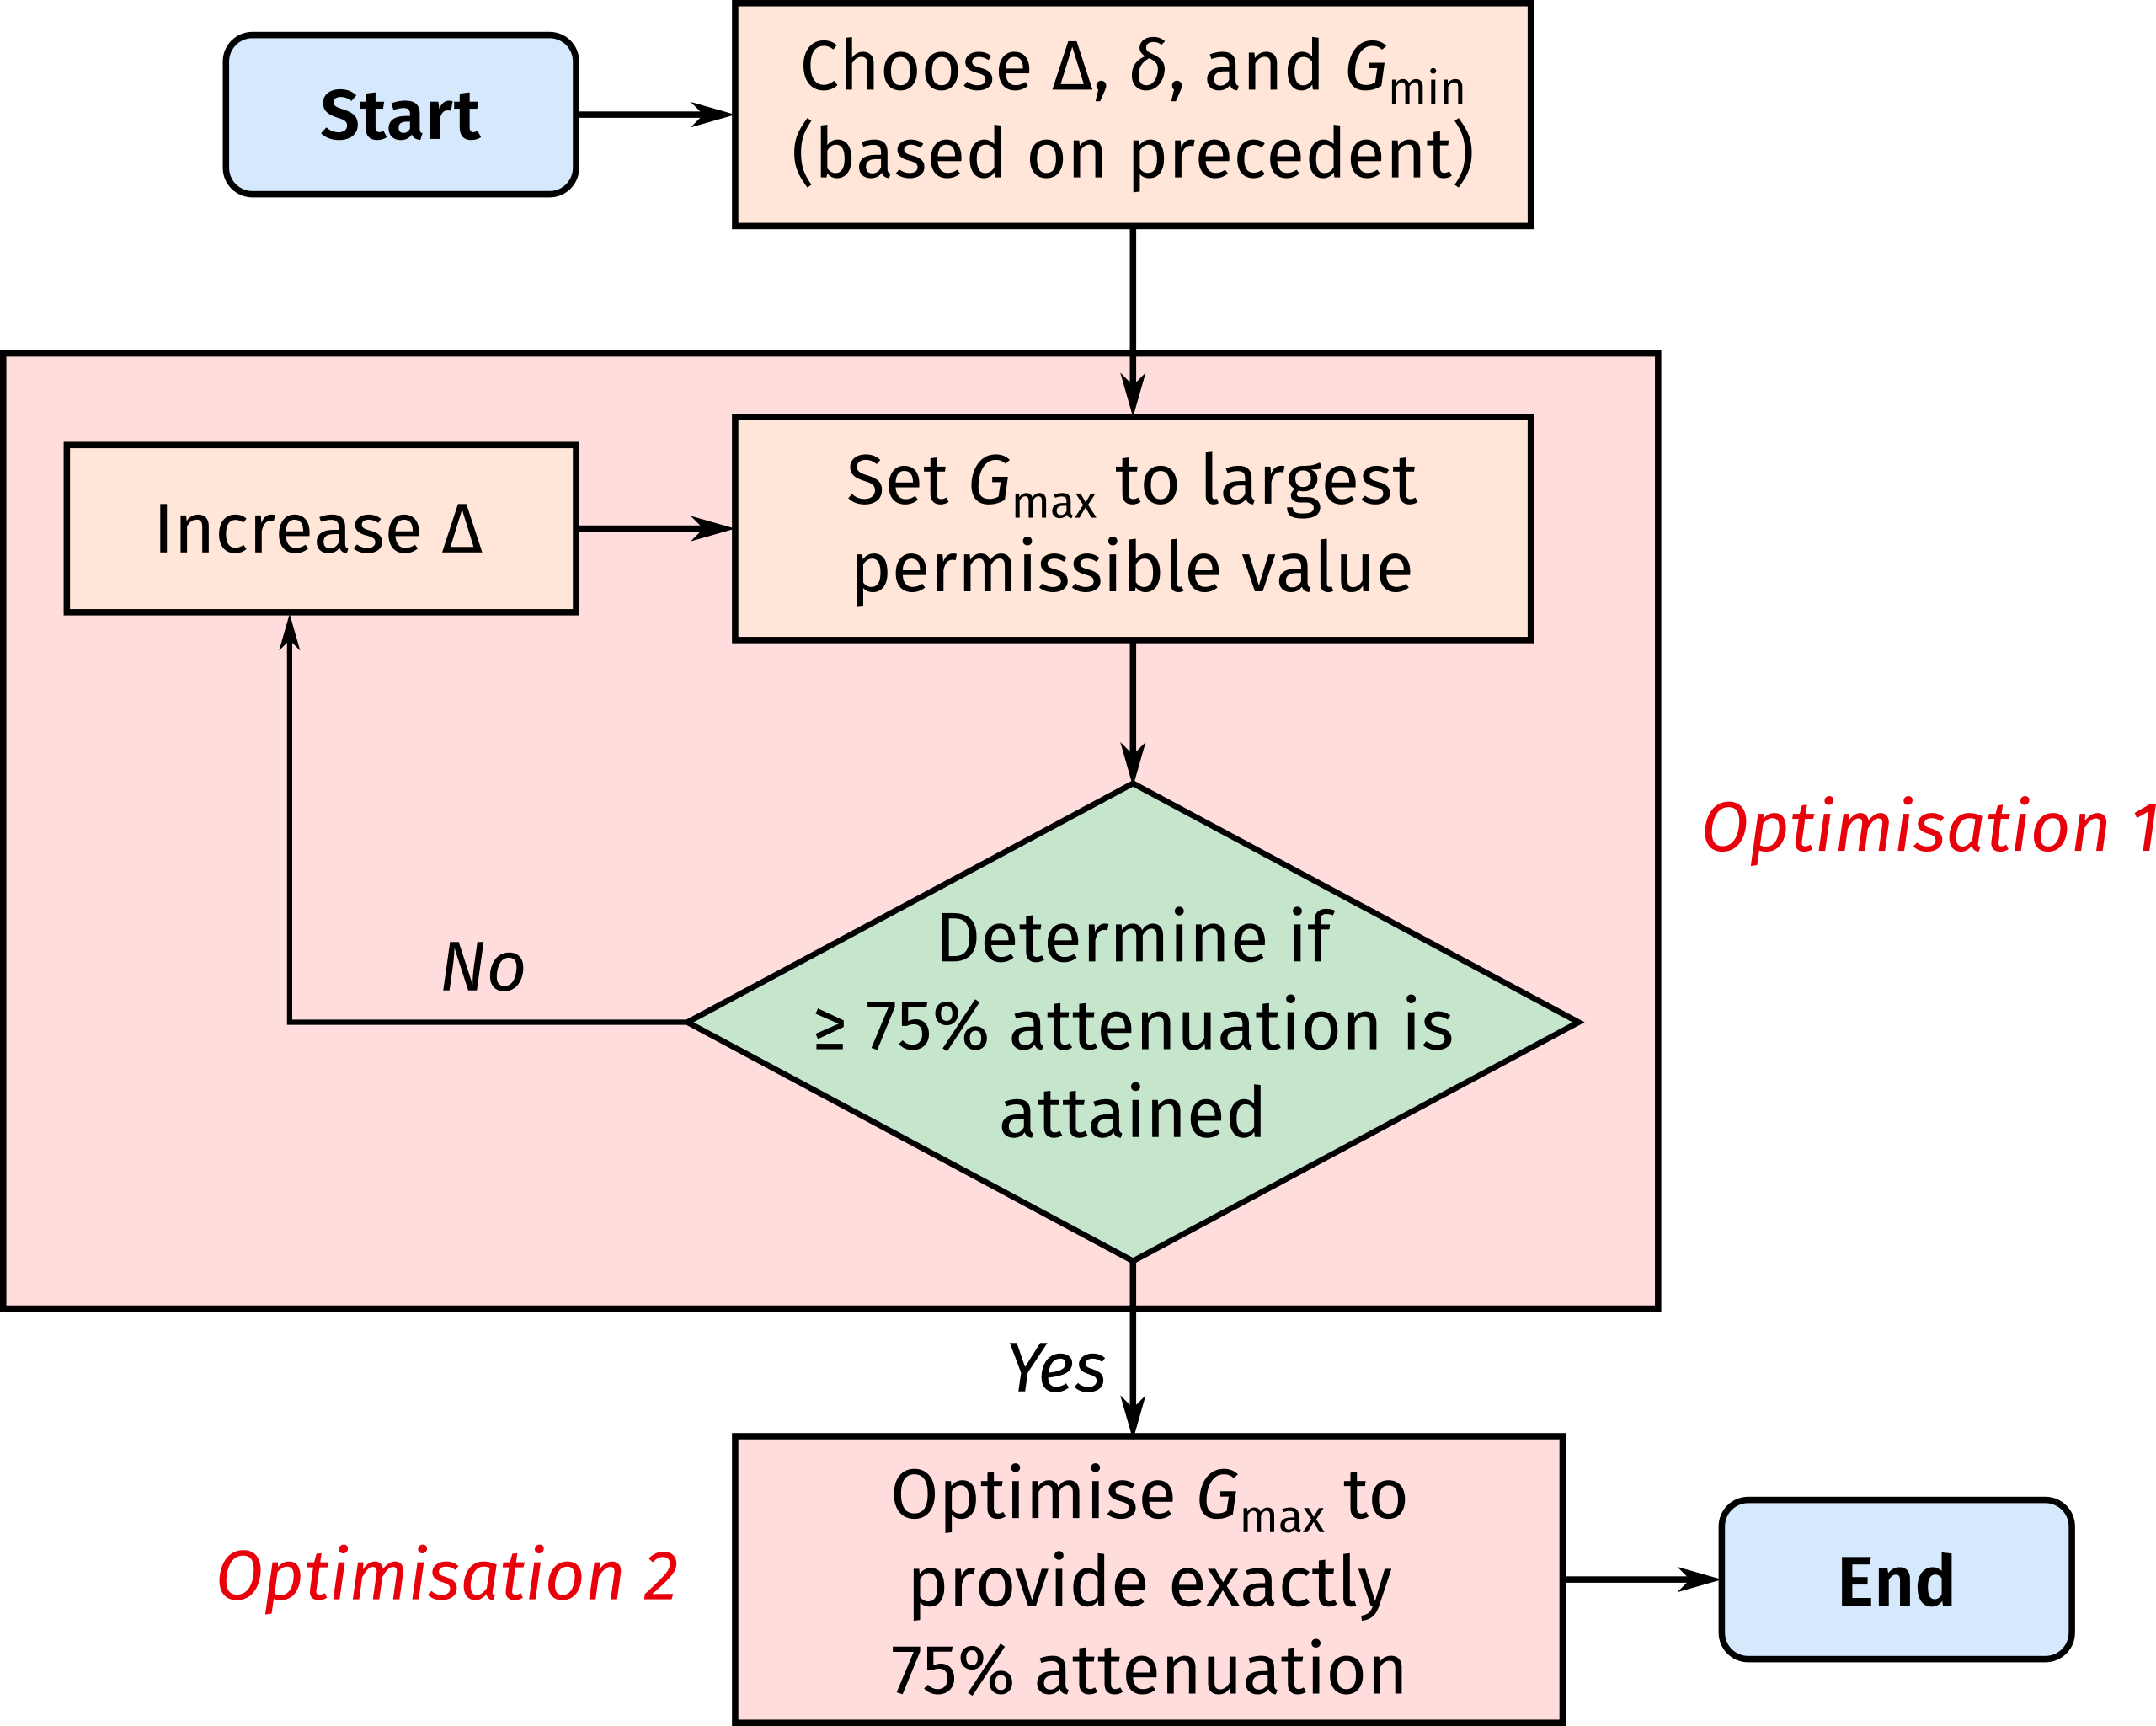
\includegraphics[]{poise/dosy_flowchart.png}%
    \caption[Flowchart for DOSY parameter optimisation]{
        Flowchart for DOSY parameter optimisation. In fact, this consists of two subproblems which can be individually solved using POISE.
    }
    \label{fig:dosy_flowchart}
\end{figure}

The DOSY optimisation procedure uses a 1D pulse programme throughout: this should essentially be a single increment of the desired 2D DOSY experiment.%
\footnote{1D versions of most DOSY variants are available in the TopSpin standard library, but can also be easily obtained by disabling the gradient incrementation in the 2D versions.}
In this work, I specifically used the Oneshot DOSY sequence\autocite{Pelta2002MRC} (\cref{fig:poise_dosy_pulseq_oneshot}): this sequence has the advantage of not requiring onerously long phase cycles, which would otherwise lead to very long FEs and optimisations.\footnote{However, using \textit{too few} scans leads to inaccuracies in the diffusion coefficients.\autocite{Pelta2002MRC} I chose to use 4 scans per FE here.}
In principle, though, the optimisation can be run with any DOSY variant, including convection-compensated sequences: the \texttt{dosy\_opt.py} wrapper script is sufficiently general that only minor modifications are needed to use it with other DOSY sequences.

The first optimisation subproblem is the determination of an appropriate diffusion delay $\Delta$.
Since larger diffusion delays lead to a greater loss of signal through $T_1$ relaxation, as well as more convection\autocite{Swan2015JMR}, $\Delta$ should always be kept as short as possible.%
\footnote{In hindsight, it would likely have been better to increase $\delta$ instead: this would also have a larger effect as the attenuation depends quadratically on $\delta$ but only linearly on $\Delta$. Care must be taken to not increase $\delta$ beyond what the spectrometer can tolerate, though.}
Thus, the wrapper script should always be started with the smallest value of $\Delta$ which is sensible for the sample under study: in the present case, I used an initial value of \qty{50}{\ms}.
The next step is to determine whether using the full range of available gradient amplitudes leads to sufficient attenuation (which I defined to be 75\%), relative to the first increment of the DOSY acquired using $G_\text{min}$.
This involves setting $G_\text{max}$ to the largest permissible value (for the Oneshot sequence, this is 80\%), then calculating a cost function $f_\text{dosy,aux}$:
\begin{equation}
    \label{eq:dosy_aux_cf}
    f_\text{dosy,aux} = \frac{\sum_i S_i(G_\text{max})}{\sum_i S_i(G_\text{min})} - 0.25.
\end{equation}
In the fraction, the numerator represents an integral over some region of the spectrum acquired with $G_\text{max}$, and the denominator an integral over the same region for the spectrum acquired with $G_\text{min}$.
If the attenuation is sufficient, then $f_\text{dosy,aux}$ will be negative.
In order for the wrapper script to monitor this cost function, POISE is instructed to perform an `optimisation' with only one function evaluation, using the \texttt{-\phantom{}-maxfev 1} flag: essentially, POISE is being used here purely as a way of evaluating the cost function $f_\text{dosy,aux}$.%
\footnote{Of course, this cost function evaluation could just be done in the wrapper script itself. In fact, it would likely be simpler to do so. But there is one clear benefit of doing it in this rather circuitous route: POISE allows the user to write cost functions in Python 3.}
At each point, POISE stores the value of $f_\text{dosy,aux}$ in the \texttt{TI} parameter, allowing the wrapper script to check it.
If the value of $f_\text{dosy,aux}$ is negative, then the wrapper script moves on to the next subproblem.
However, if it is still positive, then there is no way the desired attenuation can be accomplished using the gradient strengths available.
Thus, $\Delta$ is increased by a fixed amount (\qty{50}{\ms} in this case), and the sub-optimisation step repeated.\footnote{If sample spinning is used, then this incrementation of $\Delta$ needs to be chosen carefully, as the diffusion delay should always correspond to an integral number of rotations.}

Once a suitable value of $\Delta$ has been found, the script then searches for the correct value of $G_\text{max}$ in order to provide the `correct' amount of attenuation (in this case, 75\%).
This is done through a conventional POISE optimisation, where the cost function is
\begin{equation}
    \label{eq:dosy_cf}
    f_\text{dosy} = |f_\text{dosy,aux}| = \left| \frac{\sum_i S_i(G_\text{max})}{\sum_i S_i(G_\text{min})} - 0.25 \right|.
\end{equation}
The absolute value here makes sure that the optimisation converges to the value of $G_\text{max}$ which gives \textit{precisely} a 75\% attenuation, no more, and no less.
At this point, the wrapper script reports the appropriate values of $\Delta$ and $G_\text{max}$, and then exits; these values can then be used to set up a DOSY experiment (e.g.\ using the \texttt{dosy} TopSpin AU programme).

Before presenting some results, it is worth contemplating what would happen if the sample under study contained a mixture of different molecules, as would often be the case in DOSY experiments.
Assuming that the integrals $\sum_i S_i$ are taken over the entire spectrum, the parameters thus obtained would then be `compromise values' which are weighted more heavily towards the major component(s) in the sample.
This spectral region being evaluated can be changed by the user (via the \texttt{dpl} command), but that relies on some knowledge of the sample being studied.
Thus, in this case, our best hope is that the `compromise' parameters obtained are \textit{good enough} for all the components in the mixture.
Obviously, this can hardly be guaranteed, and the larger the difference in the diffusion coefficients of the constituent species, the more prone this approach is to failing.

In my defence, any script which seeks to optimise DOSY parameters must account for the presence of mixtures in some way, for example by identifying rapidly- and slowly-diffusing species.
This is therefore not truly an issue with POISE \textit{per se}, but rather with the approach taken in the wrapper script.
(For example, if the wrapper script can identify distinct resonances which have different attenuation profiles, then POISE could be used to perform individual optimisations on each of these.)
Nevertheless, for this reason, I refrain from claiming that the work in this section constitutes a \textit{full} method for automating DOSY.%
\footnote{Doing such an endeavour proper justice would anyway have required rather more time in my DPhil and more space in this thesis.}
I am more comfortable labelling this as a demonstration of how POISE can be integrated into larger procedures---for example, in the setup of single-component DOSY experiments.


\subsubsection{Optimisation results}

The DOSY optimisation procedure described above was tested on the sample of andrographolide (in DMSO-$d_6$.
Despite this being a single-component sample, it does at least have some mildly interesting behaviour, in that the exchangeable \ch{OH} protons have a larger apparent diffusion coefficient compared to the \ch{CH} protons.

As described previously, the procedure was initialised with a value of $\Delta = \qty{50}{\ms}$.
The gradient duration $\delta$, which is not modified, was set to \qty{2}{\ms}.
Invariably, the first sub-optimisation increased this diffusion delay to \qty{100}{\ms}.
Since this part only uses one function evaluation in POISE, the optimisation algorithm used does not actually matter.
However, the algorithm does matter for the second sub-optimisation (which searches for the best value of $G_\text{max}$).
This part was therefore performed five times per algorithm, in line with previous optimisations in this chapter (\cref{tbl:poise_dosy_opt2}).

\begin{table}[htb]
    \hbadness=10000
    \centering
    \begin{tabular}{ccccc}
        \toprule
        Entry & Algorithm & Optimum found (\%) & FEs  & Time taken (\unit{\s}) \\
        \midrule
        1     & NM        & 75.00              & 9    & 195--197             \\
        2     & MDS       & 75.00              & 9    & 196--197             \\
        3     & BOBYQA    & 75.00--75.60       & 8--9 & 175--197             \\
        \bottomrule
    \end{tabular}
    \caption[DOSY maximum gradient amplitude sub-optimisations]{
        Results of maximum gradient amplitude sub-optimisations for DOSY parameter setup.
        The POISE routine used here is: \mintinline[breaklines]{json}{{"name": "dosy", "pars": ["gpz1"], "lb": [20.0], "ub": [80.0], "init": [50.0], "tol": [2.0], "cf": "dosy", "au": "poise_1d"}}.
        \datacode{6A-200823}
    }
    \label{tbl:poise_dosy_opt2}
\end{table}

In this case, all three algorithms converged to the same result of $75\%$.
The full Oneshot DOSY spectrum was then acquired using these parameters of $\Delta = \qty{100}{\ms}$, $\delta = \qty{2}{\ms}$, and $G_\text{max} = 75\%$ (nominally \qty{49.3}{\gauss\per\cm} on the spectrometer used here, see \cref{tbl:spectrometers}).
The overall time taken was approximately five minutes: two for the first sub-optimisation to find $\Delta$, and three for the second sub-optimisation (as shown in \cref{tbl:poise_dosy_opt2}).
This figure may of course be larger depending on the number of scans used (here I used \texttt{DS=2} and \texttt{NS=4}), as well as the number of iterations required in the first sub-optimisation.

The resulting attenuation profiles for one \ch{CH} and one \ch{OH} peak are shown in \cref{fig:poise_diffusion_profiles}.
The apparently more slowly-diffusing \ch{CH} peak is attenuated to 28\% of its original intensity, whereas the exchanging \ch{OH} peak is attenuated to 20\%.
This is certainly a case where the `different components' have diffusion coefficients which are not too dissimilar, allowing reasonable results to be obtained.
Gaussian fitting using the modified Stejskal--Tanner equation
\begin{equation}
    \label{eq:stejskal_tanner_oneshot}
    I(G) = I(0) \exp\left\{-(\gamma\delta G)^2 D \left[\Delta - \frac{\delta(5 - 3\alpha^2)}{16} - \frac{\tau(1-\alpha^2)}{2}\right]\right\}
\end{equation}
yielded \textit{apparent} diffusion coefficients of \qty{7.411(13)e-9}{\m\squared\per\s} for the \ch{CH} peak and \qty{9.369(49)e-9}{\m\squared\per\s} for the \ch{OH} peak.
(The equation was obtained from the pulse programme provided on the University of Manchester website; here $\tau$ represents the time between the midpoints of each gradient within the bipolar pulse pair, and $\alpha$ the gradient imbalance factor as shown in \cref{fig:poise_dosy_pulseq_oneshot}.)

\begin{figure}[htb]
    \centering
    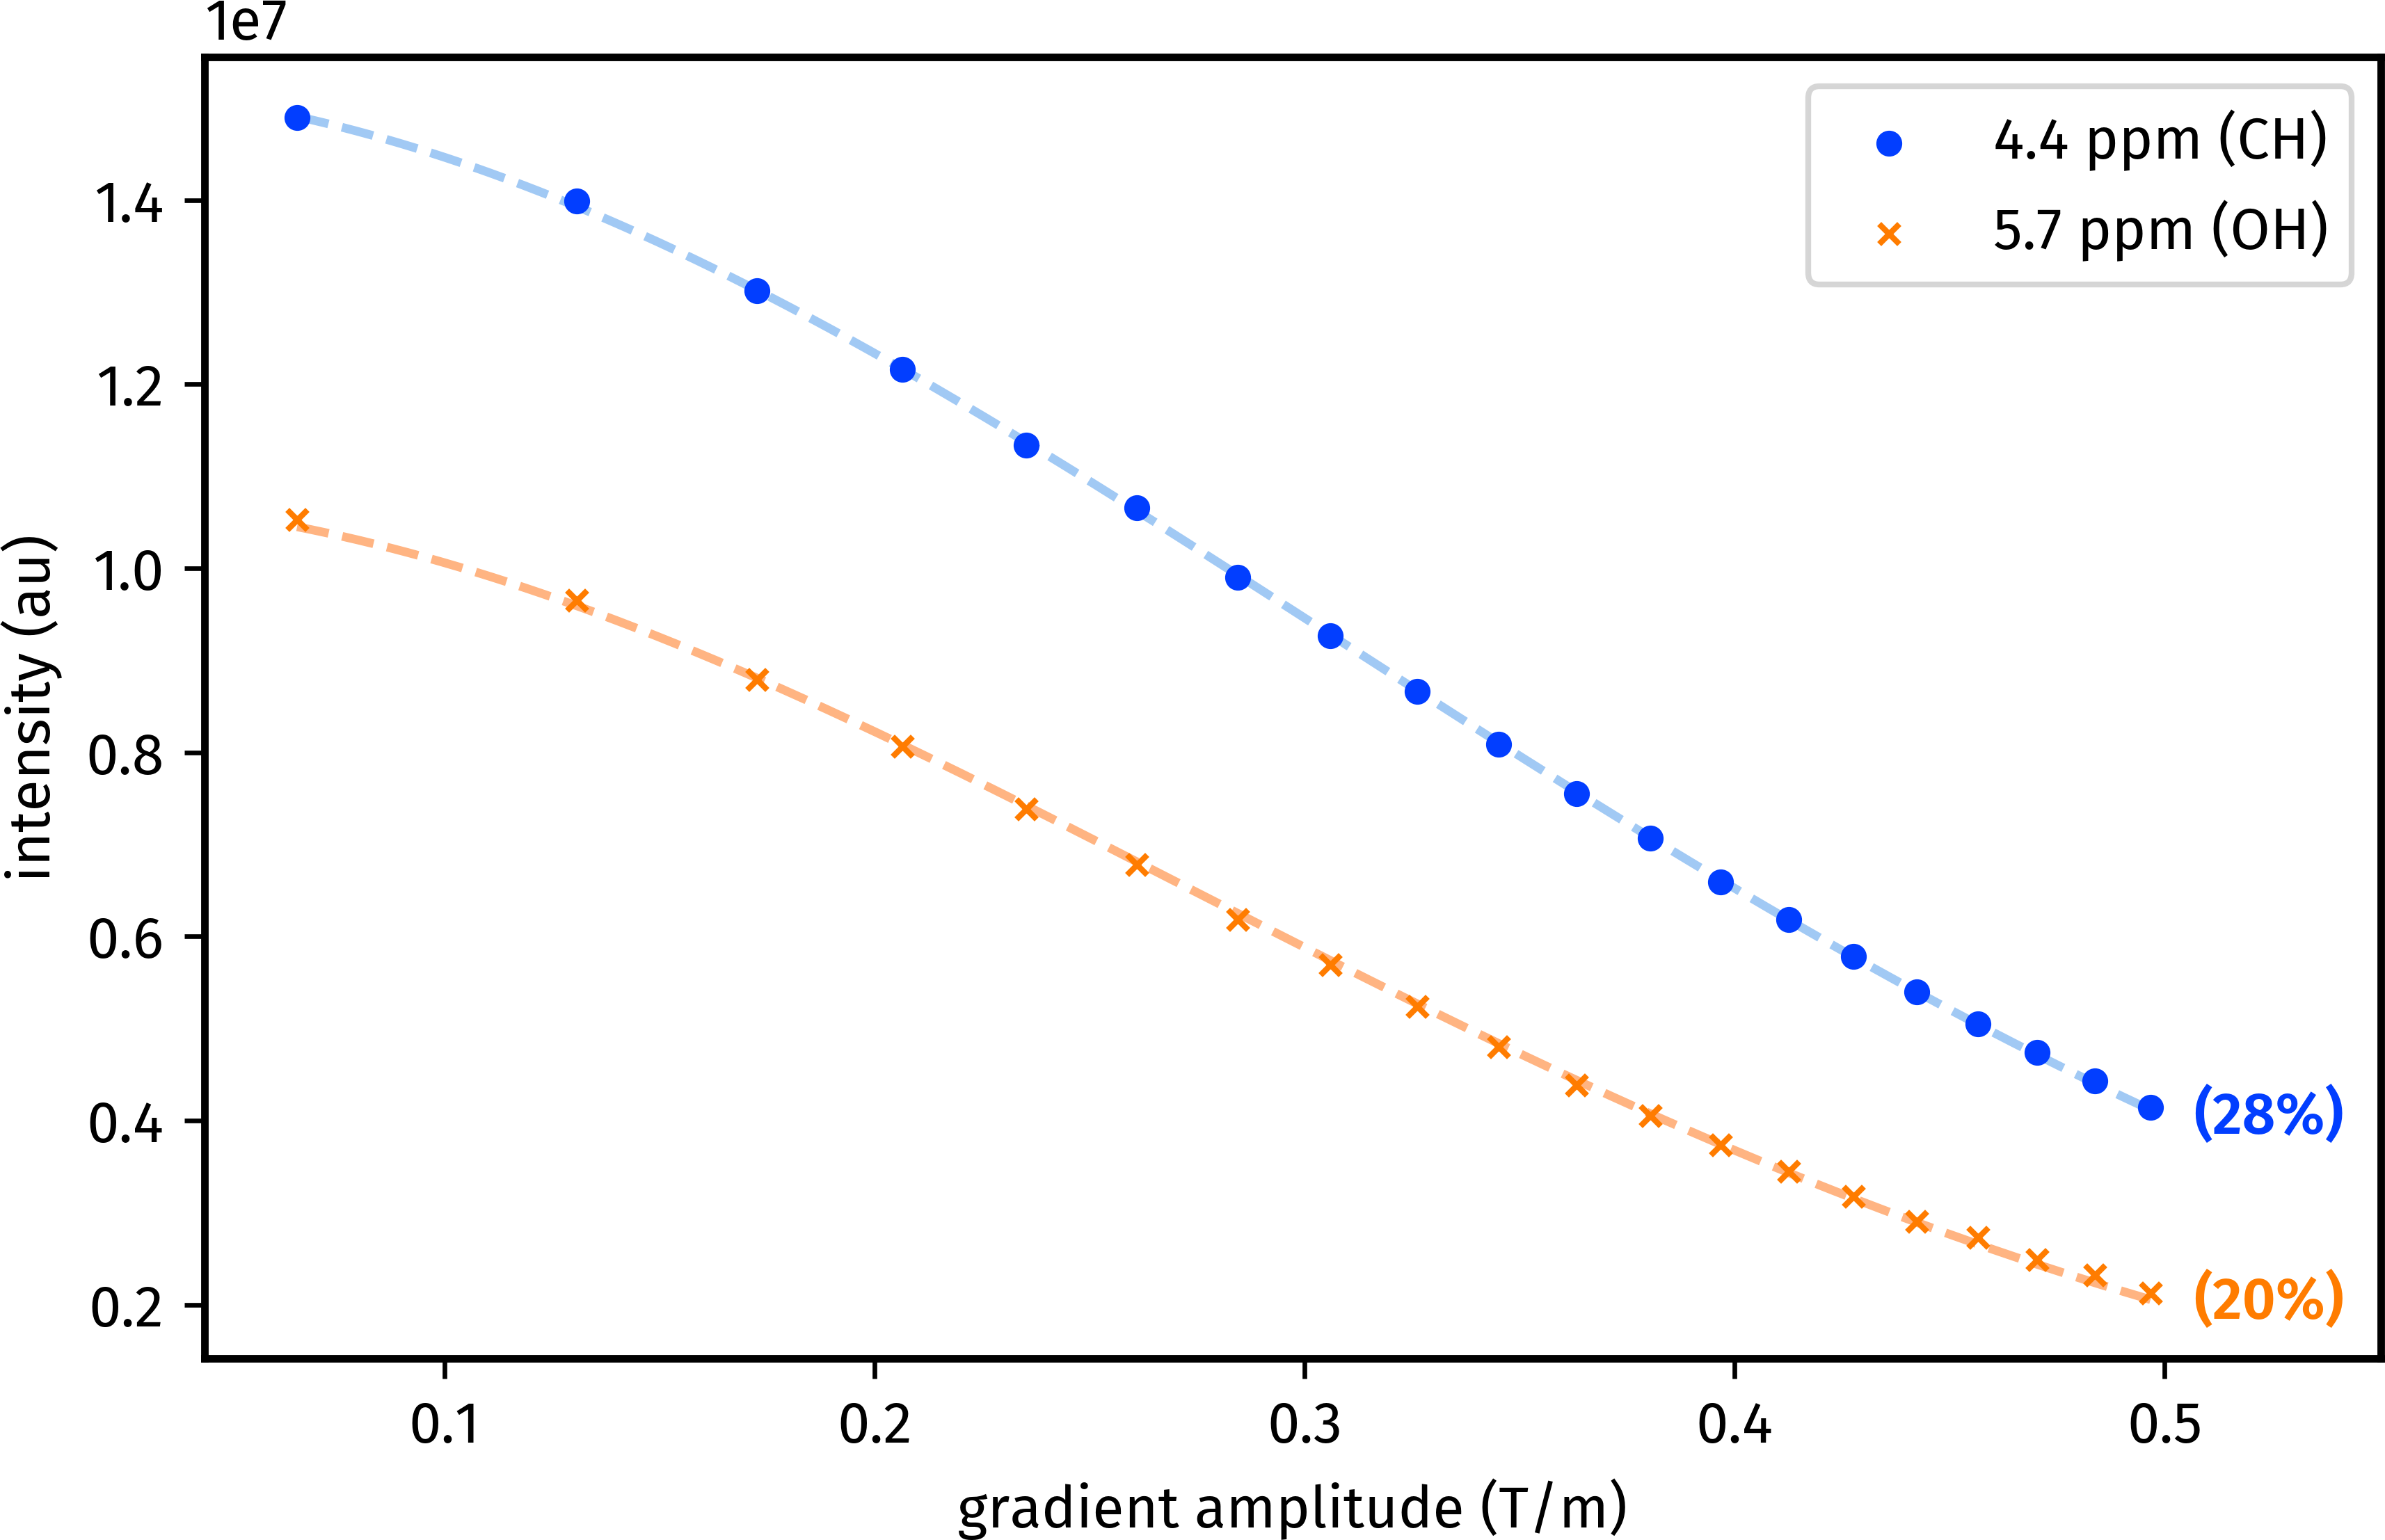
\includegraphics[]{poise/dosy_profiles.png}%
    \caption[Diffusion profiles of \ch{CH} and \ch{OH} peaks after optimisation of DOSY parameters]{
        Diffusion profiles obtained using a Oneshot experiment for a \ch{CH} peak (blue, circles) and an \ch{OH} peak (orange, crosses) in andrographolide.
        The dashed lines represent the Gaussian curves obtained through non-linear least-squares fitting (\texttt{scipy.optimize.curve\_fit}).
        \datacode{6A-200823}
    }
    \label{fig:poise_diffusion_profiles}
\end{figure}




\subsubsection{Simultaneous optimisation of $\symbf{\Delta}$ and $\symbfit{G}_\text{max}$}

It is possible---albeit inefficient, as previously mentioned---to dispense with the wrapper script entirely and perform a single optimisation of both $\Delta$ and $G_\text{max}$.
In order to ensure that $\Delta$ is not increased too much, we must add a penalty term to the cost function:
\begin{equation}
    \label{eq:dosy_2p_cf}
    f_\text{dosy,2p} = f_\text{dosy} + (\Delta / \unit{\s}) = \left| \frac{\sum_i S_i(G_\text{max})}{\sum_i S_i(G_\text{min})} - 0.25 \right| + (\Delta / \unit{\s})
\end{equation}
(where `2p' stands for two-parameter).
One significant drawback of this is that the reference spectrum $\symbf{S}(G_\text{min})$ must be reacquired every time $\Delta$ is changed: so, each FE requires twice as long as before.
For example, using the NM algorithm, the optimisation converged to $\Delta = \qty{91.6}{\ms}$ and $G_\text{max} = 79.3\%$.
Although this result is quite similar to what we had obtained before, the optimisation took over 26 minutes, over five times longer than previously.
I therefore opted not to perform the full 15 optimisations.

Curiously, BOBYQA did not work as well with this cost function: in the two times I tested it, BOBYQA converged to an `optimum' of $\Delta = \qty{225}{\ms}$ and $G_\text{max} = 50\%$.
This did yield the expected 75\% attenuation in the spectrum, but $\Delta$ is clearly rather longer than we would like it to be.
Furthermore, because of the penalty term, the value of the cost function at this point was far larger than the corresponding optimum found using the NM algorithm.
It is likely that some of the trust-region optimisation parameters must be tweaked to make this work properly, but I did not spend any further time investigating this.


\section{POISE for ESR}
\label{sec:poise__esrpoise}

In the final section of this chapter, I briefly discuss how the concept of on-the-fly optimisation may be extended to pulsed ESR spectroscopy as well.
Much of the underlying code from NMR-POISE was recycled for this, including the implementation of the three optimisation algorithms (NM, MDS, and BOBYQA).
I added only one small difference in ESR-POISE, namely, a way to control the initial size of the simplex (for NM and MDS) or the trust region radius (for BOBYQA): in NMR-POISE, this is fixed at ten times the desired optimisation tolerance.
The overall optimisation framework (\cref{fig:poise_flowchart}), as well as the concept of the optimisation routine (\cref{subsec:poise__routines}), are retained: this preserves the generality of POISE, which is probably its greatest strength.

Naturally, TopSpin-specific sections of the code had to be rewritten to instead be compatible with Bruker's Xepr software.
This in fact proved to be easier than anticipated: most of the TopSpin code could be completely deleted, because Xepr provides an API which can be accessed from external programmes such as Python 3.
Thus, ESR-POISE is in fact completely written in Python 3, and there is no need for an artificial separation between `frontend' and `backend' (which also neatly circumvents most of the issues discussed in \cref{subsec:poise__implementation}).
The Xepr-facing code was written by \JBV{} (University of Oxford) and David Goodwin (University of Southampton, formerly Oxford).

A number of applications in ESR-POISE were explored.
All ESR experimental work was done by \JBV{} and William Myers (Oxford); thus, I only provide very brief descriptions here.
The examples include:

\begin{itemize}
    \item optimisation of the signal phase in a simple spin echo experiment, by maximising the intensity of the detected echo;
    \item similarly, calibration of \ang{90} and \ang{180} pulse widths and powers in a spin echo;
    \item optimisation of an inversion pulse used on the pump channel in a DEER experiment\autocite{Pannier2000JMR}, in order to increase the modulation depth of the resulting DEER traces (which reveal dipolar couplings between electrons);
    \item calibration of shaped pulse amplitudes for CHORUS broadband excitation\autocite{Foroozandeh2019JMR,Verstraete2021JCP};
    \item compensation for resonator distortions when applying shaped pulses, again demonstrated using the CHORUS sequence.
\end{itemize}

An example of the results obtained via the latter two optimisations is shown in \cref{fig:esrpoise_comp}.
In \cref{fig:esrpoise_comp_nocomp}, the CHORUS broadband excitation experiment was run without any optimisations: the resulting spectrum (blue, solid) is compared against that obtained via a standard field sweep (grey, dashed).
Clearly, there are substantial mismatches.
\Cref{fig:esrpoise_comp_ampcomp} shows the improved performance of CHORUS after a simple optimisation of the shaped pulse amplitudes, using the spectral intensity (or the negative thereof, since we seek to maximise it) as the cost function: the POISE optimisation therefore allows for a much more accurate spectrum to be obtained.

This can be further improved, however, by compensating for distortions in the pulse shape caused by the resonator.
Typically, this is a time-consuming process, requiring the determination of a transfer function: in this case, however, it can be performed in a fully automated fashion using POISE.
The coefficients in the transfer function are used as optimisation parameters, and are used within each function evaluation to back-calculate a compensated pulse shape: the cost function used is the difference between the compensated CHORUS spectrum and the field sweep ($f_\text{diff}$, as defined in \cref{eq:ps_cf_diff}).
At the point where the cost function is minimised, the transfer function parameters will have been accurately determined.
The final compensated CHORUS spectrum is shown in \cref{fig:esrpoise_comp_resoncomp}.

\begin{figure}[htb]
    \centering
    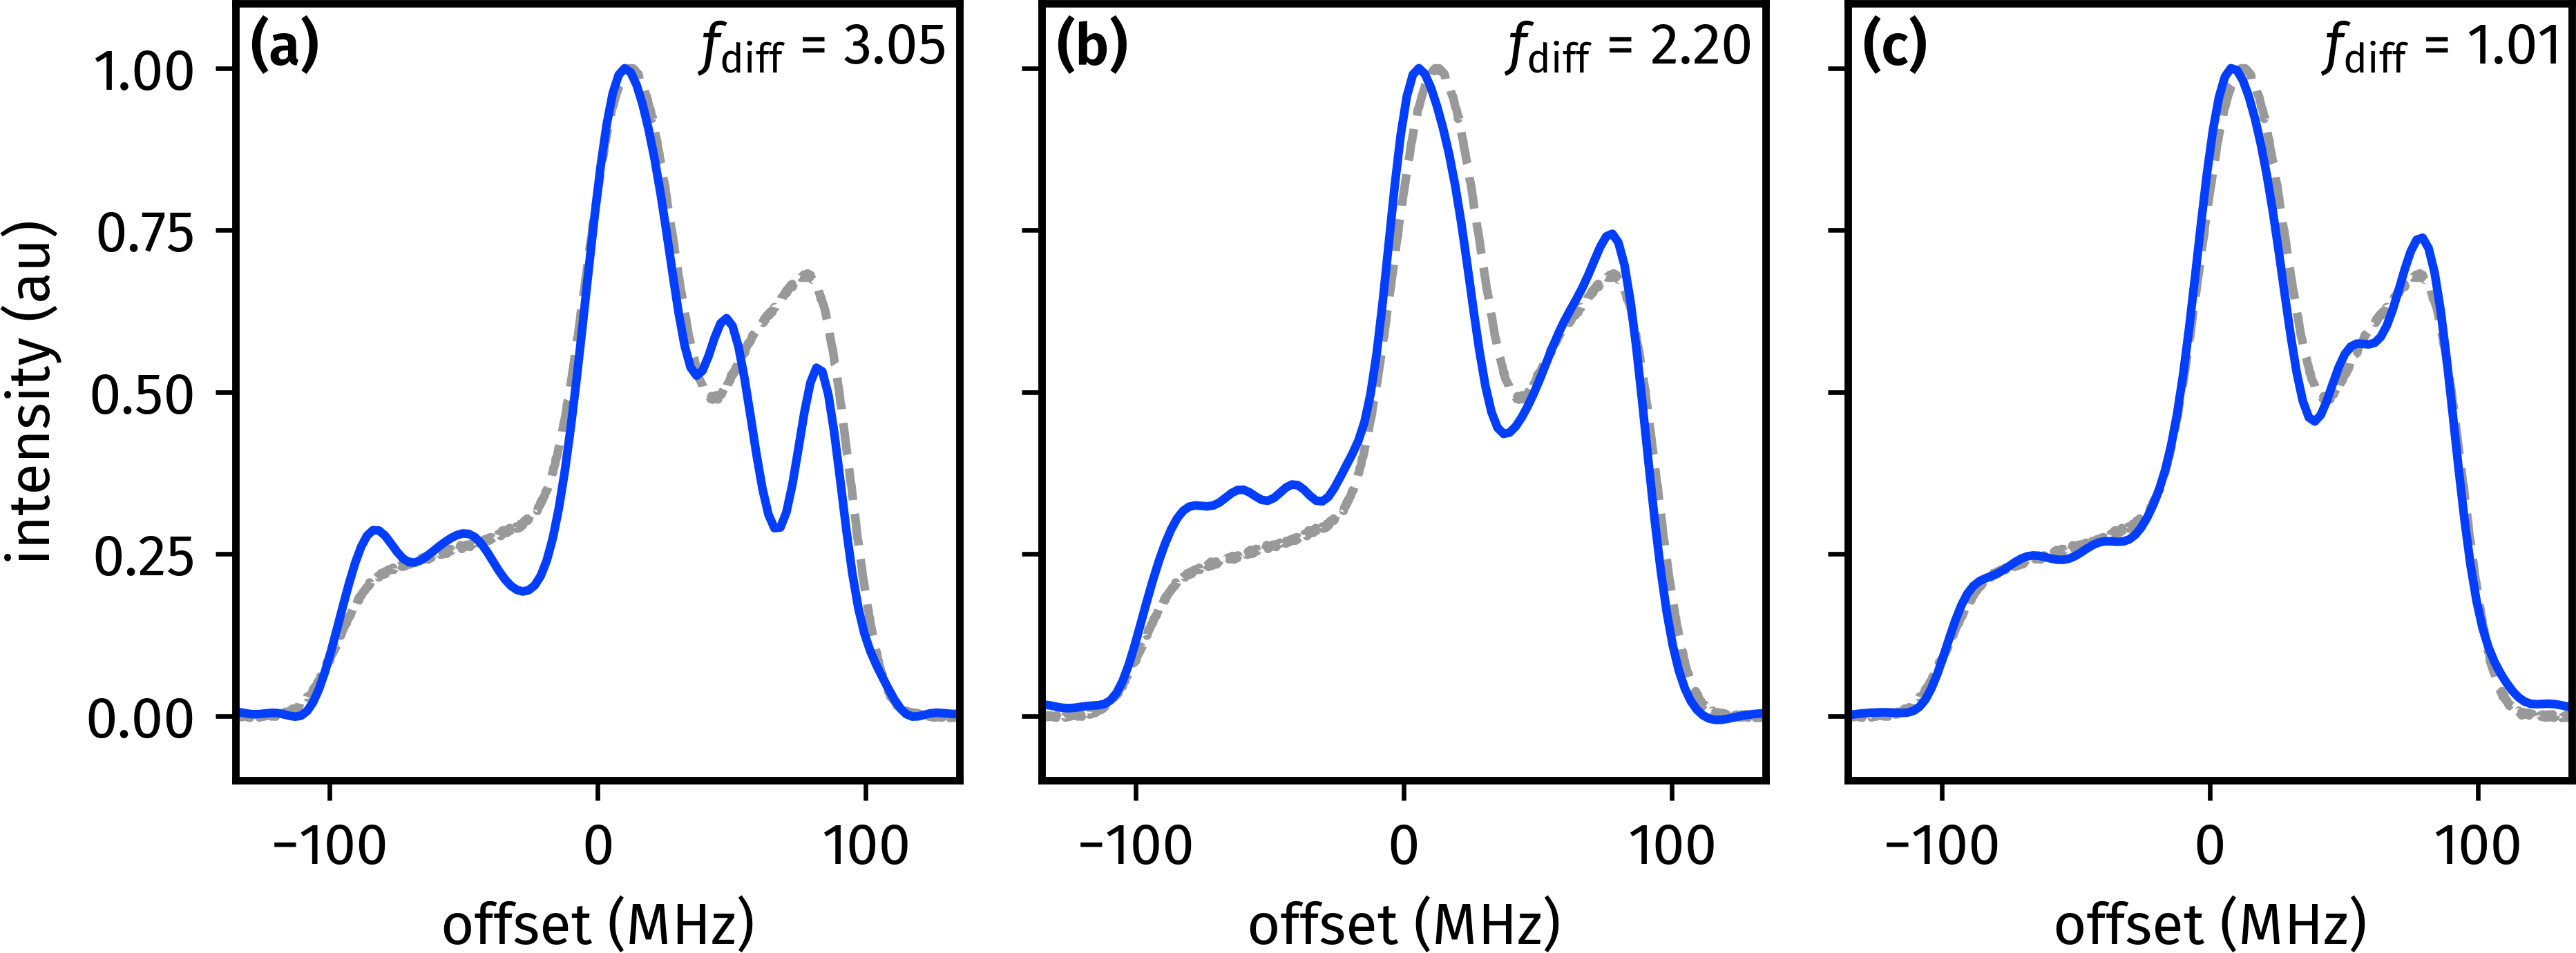
\includegraphics[]{poise/esrpoise_comp.png}%
    {\phantomsubcaption\label{fig:esrpoise_comp_nocomp}}%
    {\phantomsubcaption\label{fig:esrpoise_comp_ampcomp}}%
    {\phantomsubcaption\label{fig:esrpoise_comp_resoncomp}}%
    \caption[Comparison between CHORUS spectrum and field sweep before and after optimisation]{
        Comparison between CHORUS spectrum (blue, solid line) and field sweep profile (grey, dashed line):
        \textbf{(\subref*{fig:esrpoise_comp_nocomp})} without any optimisation of CHORUS,
        \textbf{(\subref*{fig:esrpoise_comp_ampcomp})} after optimisation of the CHORUS amplitudes, and
        \textbf{(\subref*{fig:esrpoise_comp_resoncomp})} using a compensated CHORUS pulse obtained through determination of the resonator transfer function.
        The value of $f_\text{diff}$ is indicated on each plot.
        The sample used was a bisnitroxide; further experimental details are provided in the paper.\autocite{Verstraete2022CC}
        The data used for this figure were acquired by \JBV{}.
    }
    \label{fig:esrpoise_comp}
\end{figure}


\printbibliography[heading=subbibnumbered]{}
